%% LyX 2.0.5 created this file.  For more info, see http://www.lyx.org/.
%% Do not edit unless you really know what you are doing.
\documentclass[12pt,oneside]{book}
\usepackage[T1]{fontenc}
\usepackage{geometry}
\geometry{verbose,tmargin=3cm,bmargin=3cm,lmargin=4cm,rmargin=2.5cm}
\setcounter{secnumdepth}{3}
\setcounter{tocdepth}{3}
\usepackage{prettyref}
\usepackage{refstyle}
\usepackage{float}
\usepackage{enumitem}
\usepackage{amsthm}
\usepackage{amsmath}
\usepackage{amssymb}
\usepackage{graphicx}
\usepackage{setspace}
\usepackage{esint}
\onehalfspacing
\usepackage[unicode=true,pdfusetitle,
 bookmarks=true,bookmarksnumbered=true,bookmarksopen=false,
 breaklinks=false,pdfborder={0 0 1},backref=false,colorlinks=false]
 {hyperref}

\makeatletter

%%%%%%%%%%%%%%%%%%%%%%%%%%%%%% LyX specific LaTeX commands.

\AtBeginDocument{\providecommand\eqref[1]{\ref{eq:#1}}}
\AtBeginDocument{\providecommand\secref[1]{\ref{sec:#1}}}
%% Because html converters don't know tabularnewline
\providecommand{\tabularnewline}{\\}
%% A simple dot to overcome graphicx limitations
\newcommand{\lyxdot}{.}

\floatstyle{ruled}
\newfloat{algorithm}{tbp}{loa}[chapter]
\providecommand{\algorithmname}{Algorithm}
\floatname{algorithm}{\protect\algorithmname}
\RS@ifundefined{subref}
  {\def\RSsubtxt{section~}\newref{sub}{name = \RSsubtxt}}
  {}
\RS@ifundefined{thmref}
  {\def\RSthmtxt{theorem~}\newref{thm}{name = \RSthmtxt}}
  {}
\RS@ifundefined{lemref}
  {\def\RSlemtxt{lemma~}\newref{lem}{name = \RSlemtxt}}
  {}


%%%%%%%%%%%%%%%%%%%%%%%%%%%%%% Textclass specific LaTeX commands.
\numberwithin{equation}{section}
\numberwithin{figure}{section}
\numberwithin{table}{section}
  \theoremstyle{definition}
  \newtheorem{defn}{\protect\definitionname}[section]
  \theoremstyle{plain}
  \newtheorem{thm}{\protect\theoremname}[section]
  \theoremstyle{plain}
  \newtheorem{lem}{\protect\lemmaname}[section]
 \newlist{casenv}{enumerate}{4}
 \setlist[casenv]{leftmargin=*,align=left,widest={iiii}}
 \setlist[casenv,1]{label={{\itshape\ \casename} \arabic*.},ref=\arabic*}
 \setlist[casenv,2]{label={{\itshape\ \casename} \roman*.},ref=\roman*}
 \setlist[casenv,3]{label={{\itshape\ \casename\ \alph*.}},ref=\alph*}
 \setlist[casenv,4]{label={{\itshape\ \casename} \arabic*.},ref=\arabic*}
  \theoremstyle{plain}
  \newtheorem{cor}{\protect\corollaryname}[section]

\@ifundefined{showcaptionsetup}{}{%
 \PassOptionsToPackage{caption=false}{subfig}}
\usepackage{subfig}
\makeatother

  \providecommand{\definitionname}{Definition}
  \providecommand{\lemmaname}{Lemma}
 \providecommand{\casename}{Case}
\providecommand{\corollaryname}{Corollary}
\providecommand{\theoremname}{Theorem}

\begin{document}

\title{\thispagestyle{empty}%\pagestyle{empty} %multiple pagesOptimized
Distributed Average Consensus Algorithm and its Applications }

\maketitle

\chapter*{ }

\newenvironment{acknowledgements} {\pagestyle{empty}   \begin{center} 
%\vspace*{1.5cm} 
{\Large \bfseries Acknowledgements} \end{center} 
%\vspace{0.5cm} 
\begin{quote}} {\end{quote} }

\begin{acknowledgements} 



\begin{doublespace}
 







I would like to express my gratitude to my thesis advisor Prof. Xinheng
Wang for his careful guidance and his valuable comments; his patience
and the constructive criticism helped me to organize many concepts
in a frame. His encouragement has been invaluable. thank you so much
Henry!

I would also like to thank Prof. Choi for his insightful comments
their suggestions contributed to board my view of the distributed
information system and the distributed consensus problem. Thank you
for your help and encouragement.

 

Thanks to my colleagues Frank Liu, Tommy To, Laurie Hughes, John Li.

 

At last, I would like to sincerely thank my parents, for their encouragement
and support during all phases of this work.
\end{doublespace}

\end{acknowledgements}



\chapter*{}

\newenvironment{abstract} {  \pagestyle{empty}   \begin{center}   
%\vspace*{1.5cm}   
{\Large \bfseries  Abstract}   \end{center}  
%\vspace{0.5cm}   
\begin{quote}} {\end{quote} }

\begin{abstract} 

\thispagestyle{empty}Distributed information processing has attract
more interest recently because its advantages in distributed network
than centralized method. One of the tools of distributed signal processing
is the distributed consensus algorithm. If the consensus algorithm
is to find the average value over the network, the algorithm is called
the distributed average consensus (DAC), which is an matrix iterative
algorithm to find the dominant eigenvector of the matrix. Generally,
the algorithm is required to return the result more quickly so that
the distributed system can have a higher data processing performance.
Therefore, many efforts have been devoted into the optimization of
the distributed average algorithm. However, most of the optimization
are centralized method so the system can not be optimized in a distributed
network. In addition, the existing distributed optimization algorithm
converges very slowly. 

Consequently, we proposed a distributed real-time optimization for
the DAC algorithms. The optimization has advantages in low computation
time and can work simultaneously with the consensus algorithm. Later,
an application of cloud detection is given where optimized DAC algorithms
are applied to perform the hypothesis testing. Simulation result shows
that the DAC algorithm using centralized optimization and proposed
optimization have similar performances in convergence rate, when floating
point number with double format is used and the network size is less
than 32. In addition, the performances of the detection system with
different number of sensors are plotted using relative operating characteristic
curves. It is shown that the detection system with more sensors can
have better performance. 



\end{abstract}


\pagenumbering{roman}

\tableofcontents{}

\listoffigures


\addcontentsline{toc}{chapter}{List of Figures}

\listoftables


\addcontentsline{toc}{chapter}{List of Tables}


\chapter*{Abbreviations}

%\chapter*{Abbreviations} %[List of Abbreviations]
\addcontentsline{toc}{chapter}{List of Abbreviations}
% \begin{thenomenclature} 
% \begin{abbreviations}{WidestAbbreviation} 
% \begin{itemize} 
\begin{tabular}{p{4.0cm} p{11cm}}2D &  Two Dimensional \\
3D &  Three Dimensional\\
WSNs &  Wireless Sensor Netoworks\\
DAC Algorithm &  Distributed Average Consensus Algorithm\\
FIR filter &  Finite Impulse Response Filter\\
FO-DAC Algorithm &  First-order Distributed Average Consensus Algorithm\\
HO-DAC Algorithm &  Higher-order Distributed Average Consensus Algorithm\\
CFO-DAC Algorithm &  Constant First Order Distributed Average Consensus
Algorithm\\
FT-DAC Algorithm &  Finite Time Distributed Average Consensus Algorithm\\
LLR  &  Log Likelihood ratio\\


\end{tabular}


\chapter*{Notations}

%\chapter*{Notations} %[List of Notations]
\addcontentsline{toc}{chapter}{List of Notations}
%\begin{listofsymbols} 
\begin{tabular}{p{2.5cm} p{11cm}} %\begin{abmbreviations}{WidestAbbreviation}
% \nomgroup{A}





${\cal G}$  &  Graph associated to the network \\


$\mathcal{V}$  &  Set of nodes $\mathcal{V}=\left\{ v_{1},v_{2},...,v_{n}\right\} $
in the graph ${\cal G}$\\


$\mathcal{E}$  &  Set of edges $\mathcal{E}\subseteq\mathcal{V}\times\mathcal{V}$
in the graph ${\cal G}$\\


${\cal A}$  &  Weighted adjacency associated with graph ${\cal G}$\\


$W$  &  Weight matrix of first-order DAC algorithm \\


$w_{ij}$  &  Entry of weight matrix $W$\\


$\mathbf{H}$  &  weight matrix of higher-order DAC algorithm \\


$\lambda_{i}\left(W\right)$ &  The $i^{th}$ Eigenvalue of weight
matrix $W$\\


$S\left(W\right)$  &  Spectrum of of the matrix $W$\\


\textit{$Q$ } &  Incidence matrix associated with graph ${\cal G}$\\


$L$  &  Laplacian matrix induced by ${\cal G}$\\


$l_{ij}$  &  Entry of Laplacian matrix $L$\\


$\lambda_{i}\left(L\right)$ &  The $i^{th}$ Eigenvalue of Laplacian
matrix $L=L\left({\cal G}\right)$\\


$S\left(L\right)$  &  Spectrum of the Laplacian matrix\\


$\mathbf{x}\left(k\right)$  &  Local value vector at time index
$k$\\


$x_{i}\left(k\right)$  &  Local value of node $i$ at time index
$k$\\


$\epsilon$ &  Step length of DAC algorithms\\


$\gamma$ &  Forgetting factor of DAC algorithms\\


$\epsilon_{opt,FO}$ &  Optimal step length of first-order DAC algorithms\\


$\epsilon_{opt,SO}$ &  Optimal step length of second-order DAC algorithms\\


$\gamma_{opt,SO}$ &  Optimal forgetting factor of second-order DAC
algorithms\\


$p(\lambda)$  &  The minimal polynomial of $W$ \\


$T_{i}\left(k,D_{i}\right)$  &  Toeplitz matrix in $\mathbb{R}^{D_{i}\times D_{i}}$
at $v_{i}$ with $x_{i}\left(k\right)$ as diagonal entries.\\


$\mathbf{y}_{i}\left(k,D_{i}\right)$  &  The local value history
vector at $v_{i}$ constructed by $\left[x_{i}\left(k+1\right),x_{i}\left(k+2\right),\ldots,x_{i}\left(k+D_{i}\right)\right]^{T}$
\\


$\mathbf{h}$  &  An FIR filter that can estimate the consensus value
\\


\end{tabular} 
%\end{listofsymbols}


\pagenumbering{arabic}
%\pagestyle{fancy} 
\setcounter{page}{1}


\chapter{Introduction }



































Due to the development of wireless sensor networks and the decreasing
cost of sensor nodes,  processing information that originally  acquired
by the nodes is often necessary. As any node only has a piece of local
information,  all information need to be gathered and processed at
a special node called  fusion center. This method is intuitive  and
is called centralized signal processing. 

However, fusion center is usually the most important and expense node
in the network. Once it is destroyed or failed, the whole network
breaks down. In addition, as data gathering is an energy consuming
process, centralized signal processing is limited due to energy constrain
of mobile nodes. Moreover, there is unbalance energy consumption between
nodes with different communication loads \cite{Cristescu2004}\cite{Yuen2008}. 

Distributed signal processing has become more attractive, as it can
be robust against  nodes failure or topology changes \cite{Chair1986}
. However, not all the signal processing can be distributed many processing
algorithm are still implemented by centralized method.

Distributed average consensus (DAC) algorithm is a tool for distributed
information processing. It has received significant attention recently
because of its robustness and simplicity. It is widely used in many
applications such as time synchronization \cite{Schenato2011}, rendezvous
\cite{Ren2008}, cooperative control of vehicles \cite{Yang2010},
formation control/flocking \cite{Olfati-Saber2012} and WSNs \cite{Hlinka2012}.
In these applications, it is often necessary that a group of nodes
can agree on certain quantities. 



In different applications, DAC algorithms may also need a little modification.
For example, in distributed tracking of a moving target by wireless
sensor networks. Suppose each sensor is observing the target coordinates
but the output is corrupted by independent and identically distributed
zero-mean Gaussian noise, to minimize the interference from the noise,
the sensors need to take the average of all initial values. In distributed
hypothesis testing, the goal is to find the production of the global
likelihood ratio which is the product of the local likelihood ratio.
Therefore, each sensor first calculate the log of the local likelihood
ratio and substitute it into the DAC algorithm. The average obtained
by DAC algorithm multiplied with the number of nodes in the network
is log of global likelihood ratio.

In practice, DAC algorithms also face the challenges of link failure,
time delay, dynamic network, asynchronous communication and other
practical aspects. Therefore, a simple but reliable solution sometimes
performs better. First-order DAC algorithms have been proved to be
robust against  topology changes and they play important roles in
practice \cite{Ren2007}. Its optimization in a dynamic network still
attract lots of interest \cite{Jakovetic2010}\cite{Nedic2010}. 


\section{Motivation of Research }

The research is motivated by the distributed detection of cloud detection
using WSN. One of the properties of mobile sensor nodes is the limited
energy capacity. Therefore, to minimize the power consumption of the
sensor nodes, DAC algorithm to perform the distributed signal processing
need to be optimized. In addition, the model of cloud requires a modification
because the sensor is using laser sensing technology. It emit a laser
to illuminate the cloud and collect the backscatters to sense the
cloud concentration.


\subsection{To Find a Faster DAC Algorithm. }

  

In the distributed tracking of a moving target, when the moving target
is highly dynamic or the sensors need to sample at a very high frequency,
it requires that the DAC algorithm returns the result in a short time.
Thus, many efforts have been devoted to optimize the algorithm. 

DAC algorithms can be divided into asymptotic and non-asymptotic algorithms.
For asymptotic algorithms, the optimization is to minimize the sub-dominate
eigenvalue of a weight matrix \cite{Asensio-Marco2012}\cite{Xiao2004}\cite{Xiong2010}.
 However, these optimization of DAC algorithms are centralized methods
. 

For non-asymptotic DAC algorithms, such as finite-time \cite{Sundaram2007}
and adaptive filter DAC algorithm \cite{Cavalcante2010}, the optimization
is to minimize the number of necessary iteration before a FIR filter
is estimated. Sumdaram and Hadjicostis \cite{Sundaram2007} verify
that there exists a FIR filter that can estimate the consensus value.
Cavalcante and Mulgrew \cite{Cavalcante2010} follow Sundaram and
Hadjicostis's work to propose an adaptive algorithm to find the filter.
However, they are not robust against topology changes.   Local values
over time obtained by the first-order DAC are taken as inputs of the
filter estimation algorithm for both of them. As a result, if the
network topology changes, these algorithms have to be reinitialized,
as outdated information during the filter estimation will lead to
a wrong answer.

To enable the whole system work distributively, the DAC algorithms
should be robust against topology changes and the optimization should
be distributed. 

A distributed method inspired by the gossip algorithm \cite{Boyd2006}
can be used to optimize the first order DAC but it converges very
slowly. The method involves triple nested distributed matrix iterations.
The inner iteration has to converge to a certain range so that the
iteration outside can return the right result. Thus, It is not surprising
that it could not finish in a reasonable time when the network size
is large. 

Therefore, a distributed optimization method with less computation
time is required. In addition, it is better that no additional communication
cost is required. Moreover, if the optimization algorithm and the
DAC algorithm can be executed simultaneously, then consensus process
will not be interrupted and the optimization can be running in background
to keep the optimal parameters updated in a dynamic network. 


\subsection{To Detect The Cloud Plume by Laser Sensor}

The cloud here is a group of harmful gas or particles floating in
the air. To detect the cloud, it is illuminated by a laser beam emitted
by a sensor and the backscatters (light reflected by particles) are
collected to generate signals. 

Because the laser beam penetrate the cloud, the intensity of backscatters
is the integration along the laser beam in that range. Consequently,
a new cloud plume model need to be obtained by take integration of
original Gaussian plume model along the direction of laser beam. 

Specifically, in the cloud detection application, the DAC algorithm
performs the task of distributed hypothesis testing may also have
a little modification. To find the production of the global likelihood
ratio, each sensor first calculate the log of the local likelihood
ratio and substitute it into the DAC algorithm as the initial local
value. DAC algorithm will then find the average. The average multiplied
by the number of nodes in the network is log of global likelihood
ratio.


\section{Contributions}

The main contribution of this thesis is that it proposed a distributed
real-time optimization method, which will not interrupt the constant
first-order DAC algorithm. Thus, the consensus algorithm and the optimization
method can be executed simultaneously. As a result, communication
cost and optimization initialization time can be dramatically reduced
compare to conventional distributed optimization. In addition, a least
mean square solution is obtained to mitigate the numerical error of
the optimal solution calculated by the proposed method. When using
floating point number in double format and the network size is smaller
than 32, the numerical error after mitigation does not dramatically
decline the algorithm performance. 

In addition, the proposed distributed eigenvalue estimation algorithm
could be an alternative to the estimation of algebra connectivity,
such as \cite{Yang2010}. The proposed method could obtain the result
with sufficient numerical accuracy. Matrix iterations only need to
be executed for times in order of $n$. 

Moreover, we propose a generalized finite-time DAC algorithm, which
does not require knowledge of network topology but will estimate the
necessary parameters during the iteration. Compared to the distributed
algorithm introduced in \cite{Sundaram2007}, it doesn't require the
re-initialization of the constant first-order DAC algorithm for several
times. Therefore, total data transmission in all iterations can be
reduced. However, re-initialization can be introduced if the consensus
value requires to have high accuracy 

Finally, a modified Gaussian plume models is presented, which is the
integration of the original Gaussian plume model along the laser beam
to simulate the laser penetration. This Gaussian plume model can only
describe the mean of the cloud concentration. However, a real cloud
cloud concentration is actually a random process. To reveal  the dynamics
and turbulence properties of the cloud plume, a 3D cloud animation
is implemented with the computer graphic technology \cite{He2011}. A
bunch of the simulated cloud plumes is generated for algorithm testing
and detection.




\section{Outline}

This thesis is structured as follows: Chapter  \ref{sec:Consensus-problem-on}
is the review of some asymptotic and non-asymptotic DAC algorithms,
as well as some distributed signal processing methods based on DAC
algorithm. In chapter  \ref{sub:Finite-time-Consensus-on}, a generalized
finite-time DAC algorithm will be presented. Compared to the previous
version of finite-time DAC, the number of iteration can be reduced.
In chapter \ref{sec:Online-Optimization-of}, a distributed real-time
optimization method to increase the convergence rate of asymptotic
DAC algorithms. Finally, a distributed detection of cloud plume using
wireless sensor networks and the DAC algorithm will be introduced
in chapter \ref{sec:DAC-Implementation:-Distributed}. Chapter \ref{sec:Conclusion-and-Future}
concludes this thesis and gives out the direction of further work.



\chapter{\label{sec:Consensus-problem-on}Background of DAC}


\section{Prelimilary}

Consider a connected graph $\mathcal{G}=\left(\mathcal{V},\mathcal{E},{\cal A}\right)$
be a weighted digraph (or undirected graph) consisted by a set of
nodes $\mathcal{V}=\left\{ v_{1},v_{2},...,v_{n}\right\} $, a set
of edges $\mathcal{E}\subseteq\mathcal{V}\times\mathcal{V}$ and a
\textit{weighted adjacency matrix} ${\cal A}=\left[a_{ij}\right]$.
The edge $\left(v_{i},v_{j}\right)\in\mathfrak{\mathcal{E}}$ is a
ordered pair of distinct nodes, associated with an element in the
adjacency matrix ${\cal A}$, i.e. $\left(v_{i},v_{j}\right)\in\mathfrak{\mathcal{E}}\Leftrightarrow a_{ij}$.
For $v_{i}$, its set of communication neighbors is denoted by $\mathcal{N}_{i}=\text{ }\left\{ v_{j}\in{\cal V}|\left(v_{i},v_{j}\right)\in\mathcal{E}\right\} $.
And $\left|\mathcal{N}_{i}\right|$ denotes the number of neighbors
of $v_{i}$. We assume $a_{ij}=0$, if $v_{j}\notin{\cal N}_{i}$
(note that $a_{ii}=0$, as $v_{i}\notin{\cal N}_{i}$) for all $v_{i}\in\mathcal{V}$.
Any node $v_{i}$ can only transmit information to other nodes that
belong to the neighbors set. 

For each edge $e_{k}=\left(v_{i},v_{j}\right)\in{\cal E}$, we arbitrarily
choose one end of $e_{k}$ to be positive and another to be negative.
The\textit{ incidence matrix} $Q=Q\left({\cal G}\right)\in\mathbb{R}^{n\times\left|{\cal E}\right|}$
is defined by 
\[
Q=\left(q_{ik}\right)=\begin{cases}
1 & \mbox{if }v_{i}\mbox{ is the positive end of }e_{k}\\
-1 & \mbox{if }v_{i}\mbox{ is the negative end of }e_{k}\\
0 & \mbox{otherwise}
\end{cases}
\]
The \textit{Laplacian matrix} of the graph ${\cal G}$ is defined
by $L=L\left({\cal G}\right)=QQ^{\mathrm{T}}$. In fact $L$ is independent
of the choice of positive ends of the edges. It is a symmetric, positive
semidefinite, singular matrix \cite{Russell1994}.

The \textit{Laplacian spectrum} of a graph \cite{Das2004} is denoted
by 
\[
S\left(L\right)=\left\{ \lambda_{1}\left(L\right),\lambda_{2}\left(L\right),\ldots,\lambda_{n}\left(L\right)\right\} 
\]
where $\lambda_{i}\left(L\right)$ is the eigenvalue of $L$ . When
refer to multiple matrix, we use $\lambda_{i}\left(A\right)$ to denote
the eigenvalues of matrix $A$. We assume these eigenvalues are ordered
non-decreasingly so that, $0=\lambda_{1}\left(L\right)\leq\lambda_{2}\left(L\right)\leq\ldots\leq\lambda_{n}\left(L\right)$.
The second smallest eigenvalue $\lambda_{2}\left(L\right)$ is called
algebraic connectivity of the graph. 

Suppose each node holds an initial scalar local value $x_{i}\left(0\right)\in\mathbb{R}$,
which can be a value that locally acquired by node representing physical
quantities such as temperature, humidity, illumination, attitude,
etc. We define the \textit{local value vector} $\mathbf{x}\left(0\right)=\left[x_{1}\left(0\right),...,x_{n}\left(0\right)\right]^{T}\in\mathbb{R}^{n}$
to represent all the initial values on the network. The network is
said to be reached a consensus if and only if $x_{i}=x_{j}$, for
all nodes $v_{i},v_{j}\in{\cal V},i\neq j$. In the other words, all
the nodes are in an agreement of a quantity, the common value of all
nodes is called the \textit{consensus value}.


\subsection{Consensus problem on Graphs}

To describe the behavior of each node or agent, suppose each node
has the following dynamics 

\begin{equation}
\dot{x}_{i}=f\left(x_{i},u_{i}\right),i\in{\cal V}
\end{equation}
and the graph (or network) is a system has the dynamics

\begin{equation}
\mathbf{\dot{x}}=F\left(\mathbf{x},\mathbf{u}\right)\label{eq:system dynamic}
\end{equation}
where $F\left(\mathbf{x},\mathbf{u}\right)$ is the columnwise concatenation
of individual dynamics $f\left(x_{i},u_{i}\right)$, for all node
$i=1,\ldots,n$. In an ad-hoc network with the mobile nodes, the topology
$G$\textbf{ }is switching and the system will updating its $F\left(\mathbf{x},\mathbf{u}\right)$
from time to time. 

The input or feedback $u_{i}$ in the node's dynamic is a function
of the historical states of node $i$ and its neighbors
\begin{equation}
u_{i}=g\left(x_{j_{1}},x_{j_{2}},\ldots,x_{j_{m_{i}}}\right)\label{eq:consensus protocol}
\end{equation}
where $j_{1},\ldots,j_{m_{i}}$ are the node indexes that belong to
the set $\left\{ i\right\} \cup{\cal N}_{i}$. \prettyref{eq:consensus protocol}
is called a consensus protocol under topology $G$. If the network
graph is not fully connected, it is said to be a distributed consensus
protocol. 
\begin{defn}
Let ${\cal X}:R^{n}\to R$ be a function of $n$ variables of $x_{1},x_{2},\ldots,x_{n}$
and let $\mathbf{x}\left(0\right)$ denotes the initial condition
of the network. The ${\cal X}$-consensus problem is a distributed
method to calculate the consensus value ${\cal X}\left(\mathbf{x}\left(0\right)\right)$
in a graph $G$. 
\end{defn}
Consensus problems can be different by their consensus values. For
instance, we give the definition of the average consensus ${\cal X}\left(\mathbf{x}\right)=\frac{1}{n}\sum_{i=1}^{n}x_{i}\left(0\right)$,
maximum consensus ${\cal X}\left(\mathbf{x}\right)=\max\left(\mathbf{x}\right)$,
minimum consensus ${\cal X}\left(\mathbf{x}\right)=\min\left(\mathbf{x}\right)$
and variance consensus ${\cal X}\left(\mathbf{x}\right)=\mbox{var}\left(\mathbf{x}\right)$
by their expressions respectively. The average consensus is a special
case of consensus problem, which computing the average of all initial
values $\overline{x}=\mbox{mean}\left(\mathbf{x}\right)=\frac{1}{n}\sum_{i=1}^{n}x_{i}\left(0\right)$
using a distributed system dynamics $\mathbf{\dot{x}}=F\left(\mathbf{x},\mathbf{u}\right)$
in a network $G$.(OK1)

We are interested in the distributed solutions of the consensus problem
as the network only allows an node to communicate with its neighbors.
We say the protocol \prettyref{eq:consensus protocol} solves the
consensus problem asymptotically if and only if there exists an asymptotically
stable state $x^{*}={\cal X}\left(\mathbf{x}\right)$ of system dynamics
\prettyref{eq:system dynamic}, which satisfying for all $\delta>0$,
there exists a time index $t^{*}>0$, such that $\left|x_{i}(t)-x^{*}\right|<\delta$
for all $t>t^{*}$ and $\forall i\in{\cal V}$.

Maximum or minimum consensus is very similar to information flooding.
Each node $v_{i}$ in the network just compare the local values held
by itself and others in ${\cal N}_{i}$, then broadcast the maximal
or minimal values. Therefore, maximum/minimum consensus can be finished
in a number of step that equal to the diameter of the graph. For upper
boundary of the diameter, see \cite{Russell1994}.

However, average consensus is more challenging problem than the maximum
(or minimum) consensus. Because, the average value is a linear combination
of all the initial states of network nodes and the condition $x_{i}^{*}={\cal X}\left(\mathbf{x}\right)$
for all $i$ has to be satisfied. In this chapter, we will discuss
the average consensus and especially its optimization problem, which
is solved distributively by discrete-time matrix iteration. Furthermore,
the variance consensus problem can be solved by two instances of average
consensus, because we have the relation $\mbox{var}\left(\mathbf{x}\right)=\mbox{mean}\left(\mathbf{x}\cdot\mathbf{x}\right)-\left[\mbox{mean}\left(\mathbf{x}\right)\right]^{2}$.
Thus, in the following of this work we focus on the average consensus
problem and the distributed average consensus (DAC) algorithms. 


\subsection{Continuous-time vs. Discrete-time Consensus}

In this section, we will show the difference between continuous-time
and discrete-time consensus 

The dynamics of the consensus protocol is given by 

\begin{equation}
\dot{x}_{i}\left(t\right)=u_{i}\left(t\right)\label{eq:continuous_time_consensus}
\end{equation}
where $u_{i}\left(t\right)$ is a consensus protocol 
\begin{equation}
u_{i}\left(t\right)=\sum_{j\in{\cal N}_{i}}a_{ij}\left(x_{j}-x_{i}\right)\label{eq:1st Order Protocol}
\end{equation}
that solves the average consensus problem ${\cal X}\left(\mathbf{x}\right)=\mbox{mean}\left(\mathbf{x}\right)$. 

The continuous-time consensus requires the nodes in a network have
dynamics in a form of differential equations. Continuous-time consensus
involves analog signals that are easily interfered by channel noise.
Consequently, the finally consensus value will be a random variable
with mean equals to the consensus value without noise and variance
proportional to the signal noise ratio. It is shown in \cite{Kar2009},
the variance is also proportional to time $t$ hence it is increasing
as the algorithm executing. 



On the other hand, discrete-time consensus only involves the quantization
error during the algorithm execution as long as the data packages
are correctly received.  Nowadays, sensor nodes with digital processing
unit becomes more cheaper, we can get more benefits from the advantages
of discrete-time consensus algorithms. Consequently, discrete-time
consensus algorithms are mainly discussed in the following of this
thesis. 


\subsubsection{Continuous-time Consensus}

The continuous-time consensus with system dynamics \prettyref{eq:continuous_time_consensus}
is a linear differential equation 
\begin{equation}
\mathbf{\dot{x}}\left(t\right)=-{\cal L}\mathbf{x}\left(t\right)\label{eq:system differential dynamics}
\end{equation}
Solving the differential equation \prettyref{eq:system differential dynamics}
will yield a continuous-time solution in an exponential matrices form
\begin{equation}
\mathbf{x}\left(t\right)=\exp\left(-{\cal L}t\right)\mathbf{x}\left(0\right)\label{eq:x(t) of CT-1st-DAC}
\end{equation}
where ${\cal L}$ is called the \textit{weighted graph Laplacian}
associated with network graph ${\cal G}$, which is defined by

\begin{equation}
l_{ij}=\begin{cases}
\sum_{k=1,k\neq i}^{n}a_{ik} & j=i\\
-a_{ij} & j\neq i
\end{cases}\label{eq:Graph Laplacian def.}
\end{equation}
For a graph with 0-1 adjacency, the weighted graph Laplacian can be
denoted in another form, which is unweighted Laplacian matrix denoted
by $L$

\begin{equation}
l_{ij}=\begin{cases}
\left|{\cal N}_{i}\right| & j=i\\
-1 & j\in{\cal N}_{i}\\
0 & \mbox{otherwise}
\end{cases}\label{eq:Laplacian def.}
\end{equation}
In some literature \cite{Xiong2009a}, they use the second definition
(\prettyref{eq:Laplacian def.}) of the Laplacian matrix to analyze
the convergence rate of DAC algorithm. It is a special case when weights
$a_{ij}$ for all edges in ${\cal E}$ equal to one. Therefore, to
distinguish them, we denote the weighted graph Laplacian matrix and
the unweighted Laplacian matrix by ${\cal L}$ and $L$ respectively. 


\paragraph*{Convergence Conditions for Continuous-time Consensus}

There is some important theories for continuous-time consensus convergence
problem. To provides the necessary and sufficient conditions of the
graph Laplacian matrix so that a convergent consensus algorithm could
be carried out on the network , some result is induced from Perron-Frobenius
theorem and Gerschgorin's theorem that gives the upper and lower boundary
of the spectral radius. 


\begin{thm}
\cite{Olfati-Saber2004} \label{thm:Bounds of eig(L)-1}Let the graph
has the Laplacian matrix ${\cal L},$ denote the maximum node outdegree
of the graph by 
\begin{equation}
d_{max}=\max_{1\leq i\leq n}\left(\sum_{j=1,j\neq i}^{n}l_{i,j}\right)
\end{equation}
Then, all the eigenvalues of ${\cal L}$ are located in the following
disk,
\begin{equation}
\left|z-d_{max}\right|\leq d_{max}
\end{equation}
which is centered at $z=d_{max}+0j$ on the complex plane.\end{thm}
\begin{proof}
Based on the Gerschgorin's theorem, all the eigenvalue of ${\cal L}$
are located in the union of the disks.
\begin{equation}
\left|z-l_{i,i}\right|\leq\sum_{j=1,j\neq i}^{n}\left|l_{i,j}\right|,\ 1\leq i\leq n.\label{eq:disk Union of eig(L)-1}
\end{equation}
Since ${\cal A}=\left[a_{i,j}\right]$ is an non-negative matrix,
by the definition of Laplacian matrix, $l_{i,j}\leq0$ and $l_{i,i}=\sum_{k=1,k\neq i}^{n}a_{ik}\geq0.$
Therefore, let $d_{i}=l_{i,i}$ and 
\begin{equation}
d_{i}=\sum_{j=1,j\neq i}^{n}\left|l_{i,j}\right|
\end{equation}
 and the union of disks becomes
\begin{equation}
\bigcup_{1\leq i\leq n}\left\{ z\in\mathbb{C}:\left|z-d_{i}\right|\leq d_{i}\right\} 
\end{equation}
On the other hand, all these disks are located inside the largest
disk with radius $d_{max}$. This result ends the proof of the theorem
\end{proof}
Based on the \prettyref{thm:Bounds of eig(L)-1}, it is obvious all
the nonzero eigenvalues of ${\cal L}$ have positive real parts. This
immediately lead to a convergence theorem of the continuous-time consensus
protocol \prettyref{eq:1st Order Protocol}. Since all the nonzero
eigenvalue of $-{\cal L}$ located in the disk $\left|z+d_{max}\right|\leq d_{max}$,
and the eigenspace associated with zero is one-dimensional, the eigenvector
associated with zero eigenvalue has the form $\alpha\mathbf{1}$,
i.e. $x_{i}=\alpha$ for all $i$. This result will be very helpful
as the negative real part can guarantee that the system dynamic is
stable and convergent, see figure \ref{fig:Boundary-of-eigenvalues-1}.

We will prove that the solution given in exponential matrices form
\prettyref{eq:x(t) of CT-1st-DAC} converge to a consensus value as
$t\to\infty$ in the next. 

\begin{figure}
\hfill{}\includegraphics{\string"Graph/location of laplacian eigenvalue\string".pdf}\hfill{}\hfill{}

\caption{\label{fig:Boundary-of-eigenvalues-1}Boundary of eigenvalues of Laplacian
matrix}
\end{figure}




Considering the system dynamic $x\left(t\right)=\exp\left(-{\cal L}t\right)x\left(0\right)$.
Because $\exp\left(-{\cal L}t\right)$ is a non-negative matrix, the
Perron-Frobenius theorem tell us that $\exp\left(-{\cal L}t\right)$
has a positive real eigenvalue equals to one which is also the spectral
radius. Together with the \prettyref{thm:Bounds of eig(L)-1} which
implies that all the eigenvalues of $-{\cal L}$ have negative real
part, see figure \ref{fig:Boundary-of-eigenvalues-1}, we immediately
come to the following theorem.
\begin{thm}
Assume ${\cal G}=\left({\cal V},{\cal E},{\cal A}\right)$ is strongly
connected graph, and the associated graph Laplacian matrix ${\cal L}$
is defined in \prettyref{eq:Graph Laplacian def.}, which has only
one zero eigenvalue. Let the $u_{r}$ is the uniformed right eigenvector
and $u_{l}$ is the uniformed left eigenvector associated with the
zero eigenvalue, i.e. $Lu_{r}=0$, $u_{l}^{T}L=0$, then we have $u_{l}^{T}u_{r}=1$
and the system dynamic 
\begin{equation}
x\left(t\right)=\exp\left(-{\cal L}t\right)x\left(0\right)
\end{equation}
will have the stable state of the system dynamic given by

\begin{equation}
x\left(t\right)=Kx\left(0\right)
\end{equation}
 where K is a matrix in $R^{n}$, and $K=\lim_{t\to\infty}\exp\left(-{\cal L}t\right)=u_{r}u_{l}^{T}$. \end{thm}
\begin{proof}
Let $A=-{\cal L}$, and it has a Jordan form of $A=UJU^{-1}$. Then
we can have $\exp\left(At\right)=U\exp\left(Jt\right)U^{-1}$. Because
$A$ has all its eigenvalue except a simple zero eigenvalue have negative
real part, thus, as $t\to\infty$, all other Jordan block vanish,
and $\exp\left(Jt\right)$ converges to a matrix with only single
nonzero entry, denoted by $Q$. Since matrix $U$ contains a column
which associated with the zero eigenvalue of $A$ is $u_{r}$, similarly,
$U^{-1}$ has a corresponding row equals to $u_{l}$. By simply calculating
the equation $K=UQU^{-1}$, we can show that $K=u_{r}u_{l}^{T}$.
And the fact $U^{-1}U=I$ shows that $u_{l}^{T}u_{r}=1$ . This ends
the proof. 
\end{proof}
For the average consensus problem, it is obvious that all the elements
in $K$ must equal to $\frac{1}{n}$. This requires the graph Laplacian
${\cal L}$ satisfies the conditions: ${\cal L}\mathbf{1}=0$, $\mathbf{1}^{T}{\cal L}=0$,
where $\mathbf{1}\in R^{n}$ is an all unity vector. And the $u_{r}$
and $u_{l}$ will change into vectors with equivalent constant in
all its components. If they are uniformed, then $u_{r}=u_{l}=\frac{1}{\sqrt{n}}.$ 


\subsubsection{Discrete-time Consensus}

The discrete-time consensus with the dynamics Eq.\prettyref{eq:continuous_time_consensus}
is 
\begin{equation}
x_{i}\left(k+1\right)=x_{i}\left(k\right)+u_{i}\left(k\right)\label{eq:discre-time consensus-1}
\end{equation}
For network agents have discrete-time consensus protocol, their system
dynamics can be given in a matrix form
\begin{equation}
\mathbf{x}(k+1)=W\mathbf{x}(k)
\end{equation}
where $W=\left[w_{ij}\right]=I-{\cal L}$. We say the iteration is
convergent if there exists a vector denoted by $\mathbf{x}^{*}$,
which satisfies.

\begin{equation}
\mathbf{x}^{*}=W\mathbf{x}^{*}\label{eq:stable state iteration}
\end{equation}
Moreover, 

\begin{equation}
\mathbf{x}(k+1)-\mathbf{x}^{*}=W\left[\mathbf{x}(k)-\mathbf{x}^{*}\right]\label{eq:error vector iter. 1st}
\end{equation}
\prettyref{eq:stable state iteration} states that $\mathbf{x}^{*}$
is a right eigenvector of matrix $W$ associated with a simple eigenvalue
1. For  convergence conditions and more details about discrete-time
first-order DAC algorithm, see \prettyref{sub:DT-First-Order-DAC}. 


\section{Categories of Distributed Consensus Average Algorithm}

Distributed average consensus (DAC) algorithms is one of the most
widely used consensus algorithm.

To introduce the DAC algorithm, we may started from one of the simplest
one in their family. As shown in \prettyref{sub:DT-First-Order-DAC}.
(\prettyref{fig:Categories-of-Discrete-time} only shows the branch
of discrete-time distributed consensus algorithm. Although continuous-time
consensus algorithms have some similarities with discrete-time ones,
their performance are quite different when Gaussian white noise exists).
The first order DAC algorithm is the simplest algorithm that can solve
the consensus problem in a number of iteration. It's convergence rate
is related to the spectral radius of a graph dependent matrix. So
the optimization problem is to find the optimal matrix with minimum
spectral radius. However, global information of the graph matrix must
be available. In distributed methods, this is a quite strong condition.
Without the global information, best constant and metropolitan matrix
can be the sub-optimal solution to the consensus problem \cite{Xiao2004}.
The first order DAC algorithm is one of the asymptotic algorithms
together with higher-order DAC algorithm. The demand of higher-order
algorithm is mainly because the requirement for a fast convergence
rate is always a matter of issue. In \prettyref{sub:Discrete-High-Order},
we introduced higher-order DAC algorithm, which could have faster
convergence rate, and no additional requirement and communication
cost is required compared with first-order DAC \cite{Xiong2010}.
Therefore, it is shortly applied into practical consensus problem
after invented. (OK first half 0.5)

Some of the novel methods can solve the average consensus problem
in finite number of iterations. These methods are referred to as finite-time
consensus algorithm \cite{Sundaram2007}. It actually a very sophisticated
signal processing technique that find the asymptotically stable equilibrium
$\bar{x}$ by extrapolation, see \prettyref{sec:Finite-Time-Distributed-Consensu}.
A derivative of finite-time consensus algorithm is the adaptive filter
algorithm for average consensus . It applies an adaptive filter algorithm
to asymptotically converge the set of parameters which are required
in the computation of consensus value \cite{Cavalcante2010}. As a
contribution of this thesis, a method to calculate these necessary
parameters by inverting Toeplitz matrix is introduced in \prettyref{sub:Finite-time-Consensus-on}. 

\begin{figure}
\hfill{}\includegraphics[width=13.5cm]{\string"Graph/Categories of DAC_Nor\string".pdf}\hfill{}

\caption{\label{fig:Categories-of-Discrete-time}Categories of Discrete-time
Consensus Algorithm}
\end{figure}



\subsection*{}



\section{Asymptotic Distributed Consensus Algorithm}

The averaging consensus problem can be solved not only by DAC algorithms,
but also in many other ways, such as flooding, gossip and so on. In
the flooding algorithm, each sensor maintains a table of all sensors
values which initialize by its local value. At each iteration of the
flooding algorithm, every node exchanges the table with their neighbors.
After enough steps, which is larger than the diameter of the network.
Every node will get all the initial value of all nodes. Gossip algorithms
are asynchronous. Only one random node wakes up and randomly chooses
another node. The two nodes exchange their estimates and update to
the average of the two. 

Due to the simplicity and robustness of asymptotic distributed consensus
algorithm, it plays an important role in the practical problems. They
are already applied to network with a large number of nodes and proofed
to be robust against the topology variation. Once the network graph
is strong connected, the convergence to global consensus value is
guaranteed \cite{Ren2007}. In this section, we start from the first-order
DAC algorithm and then expand the algorithm to higher-order in order
to yields a higher the convergence rate.


\subsection{\label{sub:DT-First-Order-DAC}Discrete First Order Distributed Consensus
Algorithm}

First Order Distributed Consensus Algorithm (FO-DCA) update the local
value of node $i$ iteratively at each time-step $k$ by a weighted
sum of node\textquoteright{}s local values one time step before, given
by 

\begin{eqnarray}
x_{i}(k+1) & = & x_{i}(k)+\sum_{j\in\mathcal{N}_{i}}w_{ij}\left[x_{j}(k)-x_{i}(k)\right]\label{eq:1st iter. ni}\\
 & = & w_{ii}x_{i}(k)+\sum_{j\in\mathcal{N}_{i}}w_{ij}x_{j}(k)
\end{eqnarray}
where $k=0,1,2,...$ is the time index, $w_{ij}$ is the weight to
$x_{j}$ at node $i$, $w_{ij}=0$ if $(i,j)\notin\mathcal{E}$. Note
that we define a weight to node $i$ itself $w_{ii}=1-\sum_{j\in\mathcal{N}_{i}}w_{ij}$,
so that the sum of all weights equals to one, $\sum_{j=1}^{n}w_{ij}=1$. 

The iteration \prettyref{eq:1st iter. ni} can be written in a vector
form 

\begin{equation}
\mathbf{x}(k+1)=W\mathbf{x}(k)\label{eq:first order matrix}
\end{equation}
where $W$ is a weight matrix which refer to as the Perron matrix
induced by ${\cal G}$ \cite{Olfati-Saber2004}. This linear iteration
implies that $\mathbf{x}(k)=W^{k}\mathbf{x}(0)$ for $k=1,2,\cdots$. 

Since the initial value vector is randomly chosen, the matrix $W$
must satisfy some convergence conditions to make sure the iteration
convergent, and the convergence rate depends on the spectral radius
of matrix $W$.


\subsubsection{Convergence Conditions}

For the matrix iteration defined in \prettyref{eq:first order matrix},
the average consensus problem is to choose the weight matrix $W$,
so that for any initial value $\mathbf{x}(0)\in R^{n}$, $\mathbf{x}(k)$
converges to the vector 

\begin{equation}
\mathbf{\bar{x}}=\left(\mathbf{1}^{\mathrm{T}}\mathbf{x}(0)/n\right)\mathbf{1}=\dfrac{\mathbf{11}^{\mathrm{T}}}{n}\mathbf{x}(0)
\end{equation}

\begin{thm}
\cite{Xiao2004}\textup{\label{thm:convergence condition}$\lim_{k\rightarrow\infty}\mathbf{x}(k)=\mathbf{\bar{x}}$}
if and only if the matrix $W$ satisfie\textup{s
\begin{equation}
\lim_{k\rightarrow\infty}W^{k}=\dfrac{\mathbf{11}^{\mathrm{T}}}{n}.\label{eq:convege condition W}
\end{equation}
}Eq.\prettyref{eq:convege condition W} holds if and only if
\begin{eqnarray}
\mathbf{1}^{\mathrm{T}}W & = & \mathbf{1}^{\mathrm{T}}\label{eq: Converge condition W_Left}\\
W\mathbf{1} & = & \mathbf{1}\label{eq: Converge condition W_right}\\
\rho\left(W-\mathbf{11}^{\mathrm{T}}/n\right) & < & 1\label{eq:Converge cond. rhu<1}
\end{eqnarray}
where vector $\mathbf{1}=[1,1,\cdots1,]^{\mathrm{T}}\in R^{n}$, $\rho\left(\cdot\right)$
denotes the spectral radius of the matrix .
\end{thm}
Eq.\prettyref{eq: Converge condition W_Left} means that has a left
eigenvector $\mathbf{1}$ associated with the eigenvalue 1. This implies
that the sum of local value vector is not changed in the iteration
$\sum_{i\in\mathcal{V}}x_{i}\left(k+1\right)=\sum_{i\in\mathcal{V}}x_{i}\left(k\right)$
and the sum of each column of matrix $W$ is equal to one. Eq.\prettyref{eq: Converge condition W_right}
shows that $W$ is a row stochastic matrix and has an eigenvalue 1
with associated eigenvector $\mathbf{1}$. Both \prettyref{eq: Converge condition W_Left}
and \prettyref{eq: Converge condition W_right} together with the
convergence condition \prettyref{eq:Converge cond. rhu<1} means that
$W$ have a simple eigenvalue equals to one, and modular of all other
eigenvalues are less than one.
\begin{lem}
\textup{\label{thm:Share the eigenvalues}If $\lim_{k\rightarrow\infty}W^{k}=\dfrac{\mathbf{11}^{\mathrm{T}}}{n}$,
the matrix $W-\mathbf{11}^{\mathrm{T}}/n$ share the same eigenvalues
as matrix $W$ except the simple eigenvalue one is replaced by zero.}\end{lem}
\begin{proof}
Eq.\ref{eq: Converge condition W_Left} implies that the matrix $W$
has a left eigenvector $\mathbf{1}$ associated with eigenvalue one.
And Eq.\ref{eq: Converge condition W_right} implies that $\mathbf{1}$
is a right eigenvector of $W$ associated with eigenvalue one. The
fact that $\lim_{k\rightarrow\infty}W^{k}=\dfrac{\mathbf{11}^{\mathrm{T}}}{n}$
exists if and only if there exists a  matrix $U$ and $W$ can be
Jordan decomposition as 
\begin{equation}
W=U\left[\begin{array}{cccc}
J_{1}\\
 & J_{2}\\
 &  & \ddots\\
 &  &  & J_{m}
\end{array}\right]U^{-1}
\end{equation}
where $m$ is the number of distinct Jordan block. $J_{i}$ is the
$r_{i}$ dimensional Jordan block corresponding to eigenvalue $\lambda_{i}$,
$J_{1}=I_{r_{1}}$ is the $r_{i}$ dimensional identity matrix $\left(0\leq r_{i}\leq n\right)$
and all other Jordan block are convergent, i.e. $\rho\left(J_{i}\right)<1,2\leq i\leq m$.

Let $u_{1},u_{2},\ldots,u_{n}$ be the column of $U$ and $v_{1}^{T},v_{2}^{T},\ldots,v_{n}^{T}$
be row of $U^{-1}$. Then we have 
\begin{eqnarray}
\lim_{k\to\infty}W^{k} & = & U\left[\begin{array}{cc}
I_{r_{1}} & 0\\
0 & 0
\end{array}\right]U^{-1}\label{eq: W^k to infinity has Rank one}\\
 & = & \sum_{i=1}^{r_{1}}u_{i}v_{i}^{T}=\dfrac{\mathbf{11}^{\mathrm{T}}}{n}\label{eq:u*v=00003D11}
\end{eqnarray}
As the property of unitary matrix $U$, both $u_{i}$ and $v_{i}$
are set of orthogonal normal vectors, each $u_{i}v_{i}^{T}$ is a
matrix with rank one and matrix $\sum_{i=1}^{n}u_{i}v_{i}^{T}$ has
rank $n$. The sum $\sum_{i=1}^{r_{1}}u_{i}v_{i}^{T}$ must have rank
$r_{1}.$ Eq.\ref{eq:u*v=00003D11} shows that $r_{1}$ must equal
to one and $u_{i}v_{i}^{T}=\dfrac{\mathbf{11}^{\mathrm{T}}}{n}$,
both $u_{i}$ and $v_{i}$ are vectors with the same constant on all
components. Therefore, $W-\dfrac{\mathbf{11}^{\mathrm{T}}}{n}$ have
the same Jordan decomposition as $W$ except the Jordan block $J_{1}$
is replaced by zero, and all other Jordan block remain the same. This
completes the proof. 
\end{proof}
The convergence rate of the FO-DCA is related to the spectral radius
of matrix $W-\dfrac{\mathbf{11}^{\mathrm{T}}}{n}$. To get the maximum
convergence rate, an optimization problem to minimize the spectral
radius of the matrix could be solved \cite{Xiao2004}. 

\begin{equation}
\begin{array}{ccc}
\mbox{\mbox{Minimize }} & \rho\left(W-\frac{\mathbf{1}\mathbf{1}^{T}}{n}\right)\\
\mbox{Subject to } & \mathbf{1}^{\mathrm{T}}W=\mathbf{1}^{\mathrm{T}},\; W\mathbf{1}=\mathbf{1} & ,
\end{array}\label{eq: Opt. FO-DAC Problem}
\end{equation}
But it requires knowledge of network topology to solve the problem.
However, some non-optimal convergent weight matrices that satisfy
the condition in Eq.\prettyref{eq:convege condition W} are given
below. 


\subsubsection{First-order DAC Based On a Constant}

The simplest way to choose a weight matrix set all edges symmetric
and their weights equal to the constant $\epsilon$. A special weight
to a node itself is chosen to be $1-\epsilon\left|\mathcal{N}_{i}\right|$,
so that the sum of weights at a node is one. Therefore, the weight
matrix can be defined by the Laplacian matrix 
\begin{equation}
W=I_{n}-\epsilon L\label{eq:def. const FO-DAC}
\end{equation}
where the constant $\epsilon$ is the \textit{step length}. This kind
of DAC algorithm is called the \textit{constant FO-DAC}.

Let $\mathbf{e}_{1},\mathbf{e}_{2},\ldots,\mathbf{e}_{n}$ be the
eigenvectors of $W$ and $\lambda_{1}\left(W\right),\lambda_{2}\left(W\right),\ldots,\lambda_{n}\left(W\right)$
be the associated eigenvalues and they are ordered so that $1=\left|\lambda_{1}\left(W\right)\right|\geq\left|\lambda_{2}\left(W\right)\right|\geq\ldots\geq\left|\lambda_{n}\left(W\right)\right|$.
The largest eigenvalue $\lambda_{1}\left(W\right)$ is called the
\textit{dominant eigenvalue} and associated eigenvector $\mathbf{e}_{1}$
is called the \textit{dominant eigenvector}. 

From Eq.\prettyref{eq:def. const FO-DAC}, the eigenvalues of these
two matrix $W$ and $L$ have relationship given by $\lambda_{i}\left(W\right)=1-\epsilon\lambda_{i}\left(L\right)$.
Thus, we can determine the convergence range of $\epsilon$ in terms
of $\lambda\left(L\right)$.


\paragraph*{Choosing the step length}

For the constant FO-DAC algorithm, it is convergent, if and only if
the step length $\epsilon$ is in the range $\left(0,2/\lambda_{n}\left(L\right)\right)$.
And the optimal step length which maximize the convergence rate is
$\epsilon{}_{opt,FO}=\frac{2}{\lambda_{2}\left(L\right)+\lambda_{n}\left(L\right)}$
\cite{Xiao2004}. The boundary of the dominant eigenvalue $\lambda_{n}\left(L\right)$
can be found in \cite{Russell1994}, given by $d_{max}+1\leq\lambda_{n}\left(L\right)\leq\max\left\{ d_{u}+d_{v}\right\} $,
where $\left(u,v\right)\in{\cal E}$ , $d_{u}$ is the degree of node
$v_{u}$ and $d_{max}=\max_{v_{i}\in{\cal V}}\left|{\cal N}_{i}\right|$
is the maximum degree of nodes in the network. By Gerschgorin's theorem,
we have another upper boundary of $\lambda_{n}\left(L\right)\leq2d_{max}$,
then convergence is guaranteed if $\epsilon\in\left(0,1/d_{max}\right]$. 


\subsubsection{First Order DAC based on local degree}

Another option is Metropolis weight matrix (or local degree weight
matrix), where each weight is determined by degree of the two nodes
on the edge,

\begin{equation}
w_{ij}=\begin{cases}
\frac{1}{1+\max\left\{ d(i),d(j)\right\} }, & \mbox{if }(i,j)\in\mathit{\mathcal{E}}\\
1-\sum_{(i,k)\in\mathit{\mathcal{E}}}w_{ik}, & i=j\\
0, & \mbox{otherwise}
\end{cases}
\end{equation}
where $d(i)$ and $d(j)$ are the degrees of nodes $i$ and $j$. 

As shown above, the conventional DAC algorithm is depends on eigenvalues
of graph Laplacian matrix $\lambda_{i}\left(L\right)$ or degree of
nodes. However, in the section \ref{sub:Finite-time-Consensus-on},
we will show that the finite-time DAC algorithm in an invariant network
doesn't require these prior knowledge, if $\mathbf{x}\left(k\right)$
can be represented by a linear combination of a new normal basis defined
by eigenvectors of $W$. Thus, the weight matrix doesn't have too
much requirements and can be more easily chosen. This would be very
applicable because nodes in a distributed network usually doesn't
have any knowledge of network topology. 


\subsection{\label{sub:Discrete-High-Order}Discrete High Order Distributed Consensus
Algorithm }

Higher order Distributed Consensus Algorithm (HO-DCA) can have faster
convergence rate and potentially faster than FO-DCA. It can be easily
implemented by storing and using past data, and doesn't require additional
communication and network configuration. Moreover, HO-DAC can be regard
as a generalized form of distributed consensus algorithm \cite{Xiong2010}.
In \cite{Xiong2010}, the author assume all node can store and using
past data and define a topology-dependent matrix to update the initial
data. It involves more parameters than FO-DAC so that the optimization
problem has more degrees of freedom. When some parameters are set
to zero, the HO-DCA algorithm can reduce to the best constant FO-DAC
algorithm.

Since the convergence rate of the initial values is related to eigenvalues
of Laplacian matrix. In the optimization problem of HO-DCA, eigenvalues
of the associated graph Laplacian matrix or weight matrix must known. 

In a time-invariant, connected network, the $M-th$ high-order DAC
algorithm has the form:
\begin{eqnarray}
x_{i}(k) & = & x_{i}(k-1)-\epsilon\sum_{m=1}^{M}c_{m}(-\gamma)^{m-1}\Delta x_{i}(k,m),\label{eq:Iteration Second order x_i(k)}\\
\Delta x_{i}(k,m) & = & \sum_{j\in\mathcal{N}_{i}}\left(x_{i}\left(k-m\right)-x_{j}\left(k-m\right)\right),
\end{eqnarray}
Where $x_{i}(k)$ is the local value at node $i$ during iteration
$k$; $\mathcal{N}_{i}$ is the neighboring nodes set in which the
nodes can communicate reliably with node $i$; $\epsilon$ is a constant
step size; $M$ is the highest order number; $c_{m}$ are predefined
constants, where $c_{1}=1$ and $c_{m}\neq0\:(m>1)$; $\gamma$ is
a forgetting factor, such that $\left|\gamma\right|<1$. 

Define

\begin{equation}
\mathbf{x}(k)=\left[x_{1}(k),x_{1}(k),\ldots,x_{n}(k)\right]^{T}
\end{equation}
The Eq.\ref{eq:Iteration Second order x_i(k)} can be written in matrix
form

\begin{equation}
\mathbf{x}(k)=(I_{n}-\epsilon L)\mathbf{x}(k-1)-\epsilon\sum_{m=2}^{M}c_{m}(-\gamma)^{m-1}L\mathbf{x}(k-m)\label{eq:High Order Iter.Vec}
\end{equation}
where $L$ is the Laplacian matrix associated with the network graph.
assume $\forall k<0,\;\mathbf{x}(k)=\mathbf{x}(0)$, $\mathbf{x}(0)$
is the initial local state information for node $i$. The matrix form
states that when the forgetting factor $\gamma$ is set to zero, the
HO-DAC is reduced into the best constant FO-DAC algorithm given in 

Simulation result shows that, a higher order will have better convergence
rate, but should be trade off with the algorithm complexity and computational
cost. Also only a few improvement could be achieved if we introduce
larger than fourth order. 


\subsubsection{Convergence Rate Maximization Problem For HO-DAC}

Based on the iteration equation \ref{eq:High Order Iter.Vec}, the
$M-th$ high-order DAC algorithm in a time-invariant, connected and
undirected network, with initial local value vectors $\mathbf{x}(-M+1)=,\ldots,=\mathbf{x}(-1)=\mathbf{x}(0)$,
can be further defined by an $Mn\times Mn$ matrices
\begin{equation}
\mathbf{H}=\left[\begin{array}{cccc}
I_{n}-\epsilon L & c_{2}\gamma\epsilon L & \cdots & -c_{M}(-\gamma)^{M-1}\epsilon L\\
I_{n} & \mathbf{0}_{n\times n} & \cdots & \mathbf{0}_{n\times n}\\
\vdots & \ddots &  & \vdots\\
\mathbf{0}_{n\times n} & \cdots & I_{n} & \mathbf{0}_{n\times n}
\end{array}\right]
\end{equation}
\begin{equation}
\mathbf{J}=\left[\begin{array}{cccc}
\mathbf{K} & \mathbf{0}_{n\times n} & \cdots & \mathbf{0}_{n\times n}\\
\mathbf{K} & \mathbf{0}_{n\times n} & \cdots & \mathbf{0}_{n\times n}\\
\vdots & \vdots & \ddots & \vdots\\
\mathbf{K} & \mathbf{0}_{n\times n} & \cdots & \mathbf{0}_{n\times n}
\end{array}\right]
\end{equation}
 where $\mathbf{K}=\left(\frac{1}{n}\right)\mathbf{1}\mathbf{1}^{T}$,
and $\mathbf{0}_{n\times n}$ denotes the $n\times n$ all-zero matrix. 

The high-order DAC algorithm with initial condition $\mathbf{x}(-M+1)=,\ldots,=\mathbf{x}(-1)=\mathbf{x}(0)$
is convergent if and only if $\rho\left(\mathbf{H}-\mathbf{J}\right)<1$
\cite{Xiong2010}. Then a spectral radius minimization problem to
find the optimal $\epsilon$ and $\gamma$ for the high-order DAC
algorithm is formulated as

\begin{equation}
\begin{array}{cc}
\mbox{\mbox{Minimize }} & \rho\left(\mathbf{H}-\mathbf{J}\right)\\
\mbox{Subject to } & \epsilon,\gamma\in R
\end{array},\label{eq: High order spectral radius problem}
\end{equation}


As shown in Eq.\prettyref{eq: High order spectral radius problem},
the convergence rate maximization for high order DAC algorithm can
be cast into a spectral radius minimization problem. Finding the solution
is not easy due to we have to solve the high-order polynomial to calculate
eigenvalues. For example, the high-order polynomial of the eigenvalues
of $\mathbf{H-J}$ when $M=3$, $c_{1}=1$ and $c_{2}=1$ is 
\begin{equation}
f(\lambda)=\lambda^{3}-\left(1-\epsilon\lambda_{i}\left(L\right)\right)\lambda^{2}-\gamma\epsilon\lambda_{i}\left(L\right)\lambda+\gamma^{2}\epsilon\lambda_{i}\left(L\right)=0\label{eq: eigenvalue equation of H-J}
\end{equation}
where $\lambda_{i}(L)$ is the $i^{th}$ smallest eigenvalue of the
Laplacian Matrix \cite{Xiong2010}. 

Since each $\lambda_{i}(L),\; i=1,2,\cdots,n$ with generate one equation
which has $M$ roots, there are totally $M\times n$ eigenvalue for
$\mathbf{H-J}$. Then, problem Eq.\prettyref{eq: High order spectral radius problem}
can be written into minimize the maximum absolute value of all the
eigenvalues of $\mathbf{H-J}$. 
\begin{equation}
\begin{array}{cc}
\mbox{Minimize } & \mbox{max}\{\left|\lambda_{i}\left(\mathbf{H-J}\right)\right|\},\: i=1,2,\cdots,n\\
\mbox{Subject to } & \epsilon,\gamma\in R
\end{array},\label{eq:HO-DAC Opt. Problem}
\end{equation}



\subsubsection{Solve The Problem: Convergence rate maximization}

The convergence rate optimization problem \ref{eq:HO-DAC Opt. Problem}
of HO-DAC in undirected network can be graphically illustrated by
the \prettyref{fig:Find-minimum-rho(H)}, where the surface of $\mbox{max}\{\left|\lambda_{i}\left(\mathbf{H-J}\right)\right|\},\: i=1,2,\cdots,n$
is plotted and the optimal solution $\left(\epsilon{}_{opt},\gamma_{opt}\right)$
is marked with a star. We denote the optimized spectral radius by
$\rho_{opt}=\mbox{\mbox{min}}\rho\left\{ \left(\mathbf{H}-\mathbf{J}\right)\right\} $. 

Since the eigenvalues in the high-order polynomial \prettyref{eq: eigenvalue equation of H-J}
are network topology dependent, the solution of the problem \ref{eq:HO-DAC Opt. Problem}
may not have a unique analytical solution when the order is larger
than second. In this case, the problem will be solved numerically,
for example using steepest descent method. 

\begin{figure}
\hfill{}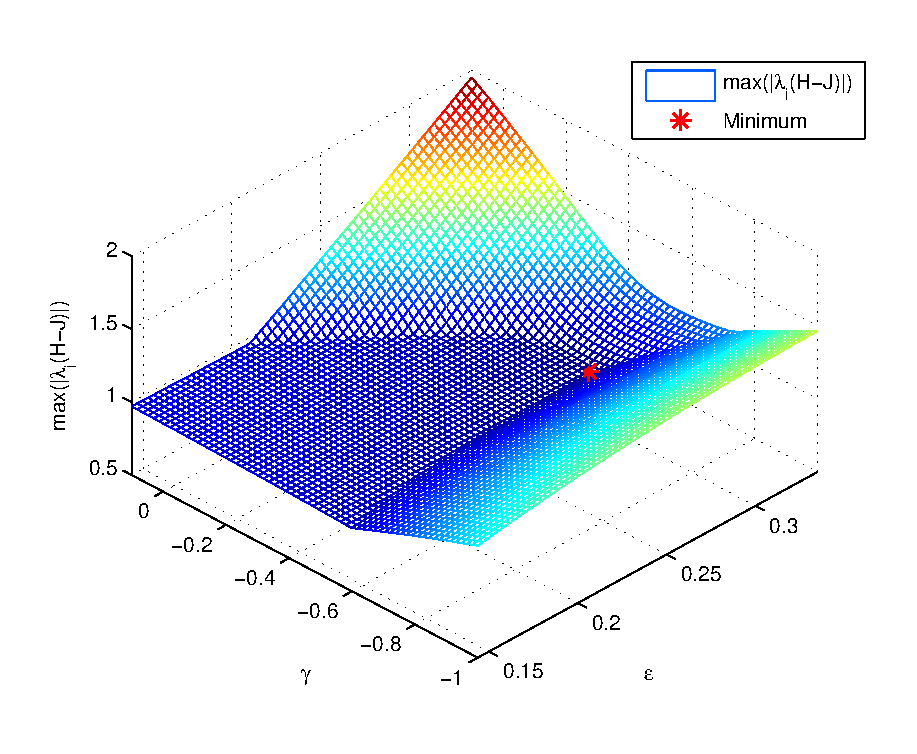
\includegraphics[height=9cm]{D:/Dropbox/PaperWork/FirstYearReport/Lyx_v/images/3order_max_lambda}\hfill{}\hfill{}\caption{\label{fig:Find-minimum-rho(H)} Illustration of Convergence rate
optimization, $\min\left\{ \mbox{max}\left[\lambda_{i}\left(\mathbf{H-J}\right)\right]\right\} ,\: i=1,2,\cdots,n$. }
\end{figure}


\begin{figure}
\hfill{}\includegraphics[height=9cm]{\string"Graph/Convergence region\string".pdf}\hfill{}\hfill{}\caption{\label{fig:Convergence-Region}Convergence Region for second order
DAC. }
\end{figure}


However, the second order DAC (SO-DAC), does exist an analytical solution.
As pointed out in \cite{Xiong2009a}, the convergence region for second
order DAC in undirected network which satisfy $\rho\left(\mathbf{H}-\mathbf{J}\right)<1$
is ${\cal R}={\cal R}_{1}\cup{\cal R}_{2}$, where 
\begin{eqnarray}
{\cal R}_{1} & = & \left\{ \frac{-1}{\epsilon\lambda_{n}\left(L\right)}<\gamma<1,0<\epsilon<\frac{1}{\lambda_{n}\left(L\right)}\right\} \\
{\cal R}_{2} & = & \left\{ \frac{-1}{\epsilon\lambda_{n}\left(L\right)}<\gamma<\frac{2}{\epsilon\lambda_{n}\left(L\right)}-1,\frac{1}{\lambda_{n}\left(L\right)}\leq\epsilon<\frac{3}{\lambda_{n}\left(L\right)}\right\} \label{eq:Def Convergence region R1 R2}
\end{eqnarray}
Fig.\ref{fig:Convergence-Region} graphically illustrate these region,
${\cal R}_{1}$ and ${\cal R}_{2}$ are defined in \prettyref{eq:Def Convergence region R1 R2}.
Note the dashed line separates the regions in which $\lambda_{n'}\left(\mathbf{H}\right),\lambda_{n"}\left(\mathbf{H}\right)$
are real and complex. In addition, optimal solution is always located
on this line. Moreover, the eigenvalues of $\mathbf{H}$ corresponding
to eigenvalue of $\lambda_{i}\left(L\right)$ is denoted by $\lambda_{i'}\left(\mathbf{H}\right)$
and $\lambda_{i"}\left(\mathbf{H}\right)$, which is 
\begin{eqnarray}
\lambda_{i'}\left(\mathbf{H}\right) & = & \frac{1}{2}\left[1-\epsilon\lambda_{i}\left(L\right)+\sqrt{\left(1-\epsilon\lambda_{i}\left(L\right)\right)^{2}+4\gamma\epsilon\lambda_{i}\left(L\right)}\right],\nonumber \\
\lambda_{i"}\left(\mathbf{H}\right) & = & \frac{1}{2}\left[1-\epsilon\lambda_{i}\left(L\right)-\sqrt{\left(1-\epsilon\lambda_{i}\left(L\right)\right)^{2}+4\gamma\epsilon\lambda_{i}\left(L\right)}\right].\label{eq:2nd-DAC lambda_H solution}
\end{eqnarray}
 

Since $\lambda_{2}\left(L\right)\leq\dots\leq\lambda_{n}\left(L\right)$,
in the convergence region of the second order DAC algorithm, the optimization
problem \prettyref{eq:HO-DAC Opt. Problem} can be equivalent to 
\[
\begin{array}{cc}
\mbox{Minimize } & \mbox{max}\{\left|\lambda_{2'}\left(\mathbf{H}\right)\right|,\left|\lambda_{2"}\left(\mathbf{H}\right)\right|,\left|\lambda_{n'}\left(\mathbf{H}\right)\right|,\left|\lambda_{n"}\left(\mathbf{H}\right)\right|\}\\
\mbox{Subject to } & \epsilon,\gamma\in R
\end{array},
\]


Finding the optimal solutions needs consideration of different combinations
of $\lambda_{2'}\left(\mathbf{H}\right),\lambda_{2"}\left(\mathbf{H}\right),\lambda_{n'}\left(\mathbf{H}\right),\lambda_{n"}\left(\mathbf{H}\right)$
when they are real value or complex value. However, for a connected
network, the $\lambda_{2'}\left(\mathbf{H}\right),\lambda_{2"}\left(\mathbf{H}\right)$
are real and $\lambda_{n'}\left(\mathbf{H}\right),\lambda_{n"}\left(\mathbf{H}\right)$
are complex values in the convergence region. When the minimum is
achieved, the following equation satisfied
\[
\left|\lambda_{2'}\left(\mathbf{H}\right)\right|=\left|\lambda_{n'}\left(\mathbf{H}\right)\right|=\left|\lambda_{n"}\left(\mathbf{H}\right)\right|
\]
Thus, by solving this equation, we have the optimal solution for second
order DAC algorithm.

\begin{eqnarray}
\epsilon{}_{opt,SO} & = & \frac{3\lambda_{n}(L)+\lambda_{2}(L)}{\lambda_{n}(L)\left[\lambda_{n}(L)+3\lambda_{2}(L)\right]}
\end{eqnarray}


\begin{equation}
\gamma_{opt,SO}=-\frac{\left[\lambda_{n}(L)-\lambda_{2}(L)\right]^{2}}{\left[\lambda_{n}(L)+3\lambda_{2}(L)\right]\left[3\lambda_{n}(L)+\lambda_{2}(L)\right]}
\end{equation}
These parameters could be floored to all sensors before the algorithm
start so that it converges faster.

Besides these results, we need to point out that the optimal solution
$\epsilon{}_{opt,SO}$ and $\gamma_{opt,SO}$ have the following relationship
\[
\gamma_{opt,SO}=\frac{\left[1-\epsilon{}_{opt,SO}\lambda_{n}\left(L\right)\right]^{2}}{-4\epsilon{}_{opt,SO}\lambda_{n}\left(L\right)}
\]
which implies the value under the square root in \prettyref{eq:2nd-DAC lambda_H solution}
is equal to zero, and $\lambda_{n'}\left(\mathbf{H}\right),\lambda_{n"}\left(\mathbf{H}\right)$
are all real values. Additionally, the optimal solution is located
just on the boundary of the regions where $\lambda_{n'}\left(\mathbf{H}\right),\lambda_{n"}\left(\mathbf{H}\right)$
is real and complex respectably, shown as dashed line in Fig. \ref{fig:Convergence-Region}. 


\subsection{Simulation and Algorithms Performance}

To test the performance of high-order DAC algorithm with different
orders, a simulation is carry out on 1000 random generated networks.
The methods and parameters of network generation are illustrated in
fig.\ref{fig:Net-N16-R0,3}. The algorithm's performance is evaluated
by the average spectral radius and average mean square error, shown
in \prettyref{fig:DAC-comparation}. 


\subsubsection{Random Network Generation}

The following is a simulation of network generation to show how the
wireless sensor networks is distributed. First, we randomly and uniformly
distribute a certain number of nodes in a unit square. Second, each
sensor randomly choose a local initial value has equally probability
density function. Finally, connect any two nodes if their satisfy
a certain communication constrains. 

\begin{figure}[h]
\hfill{}\subfloat[\label{fig:Net-N50-E200}]{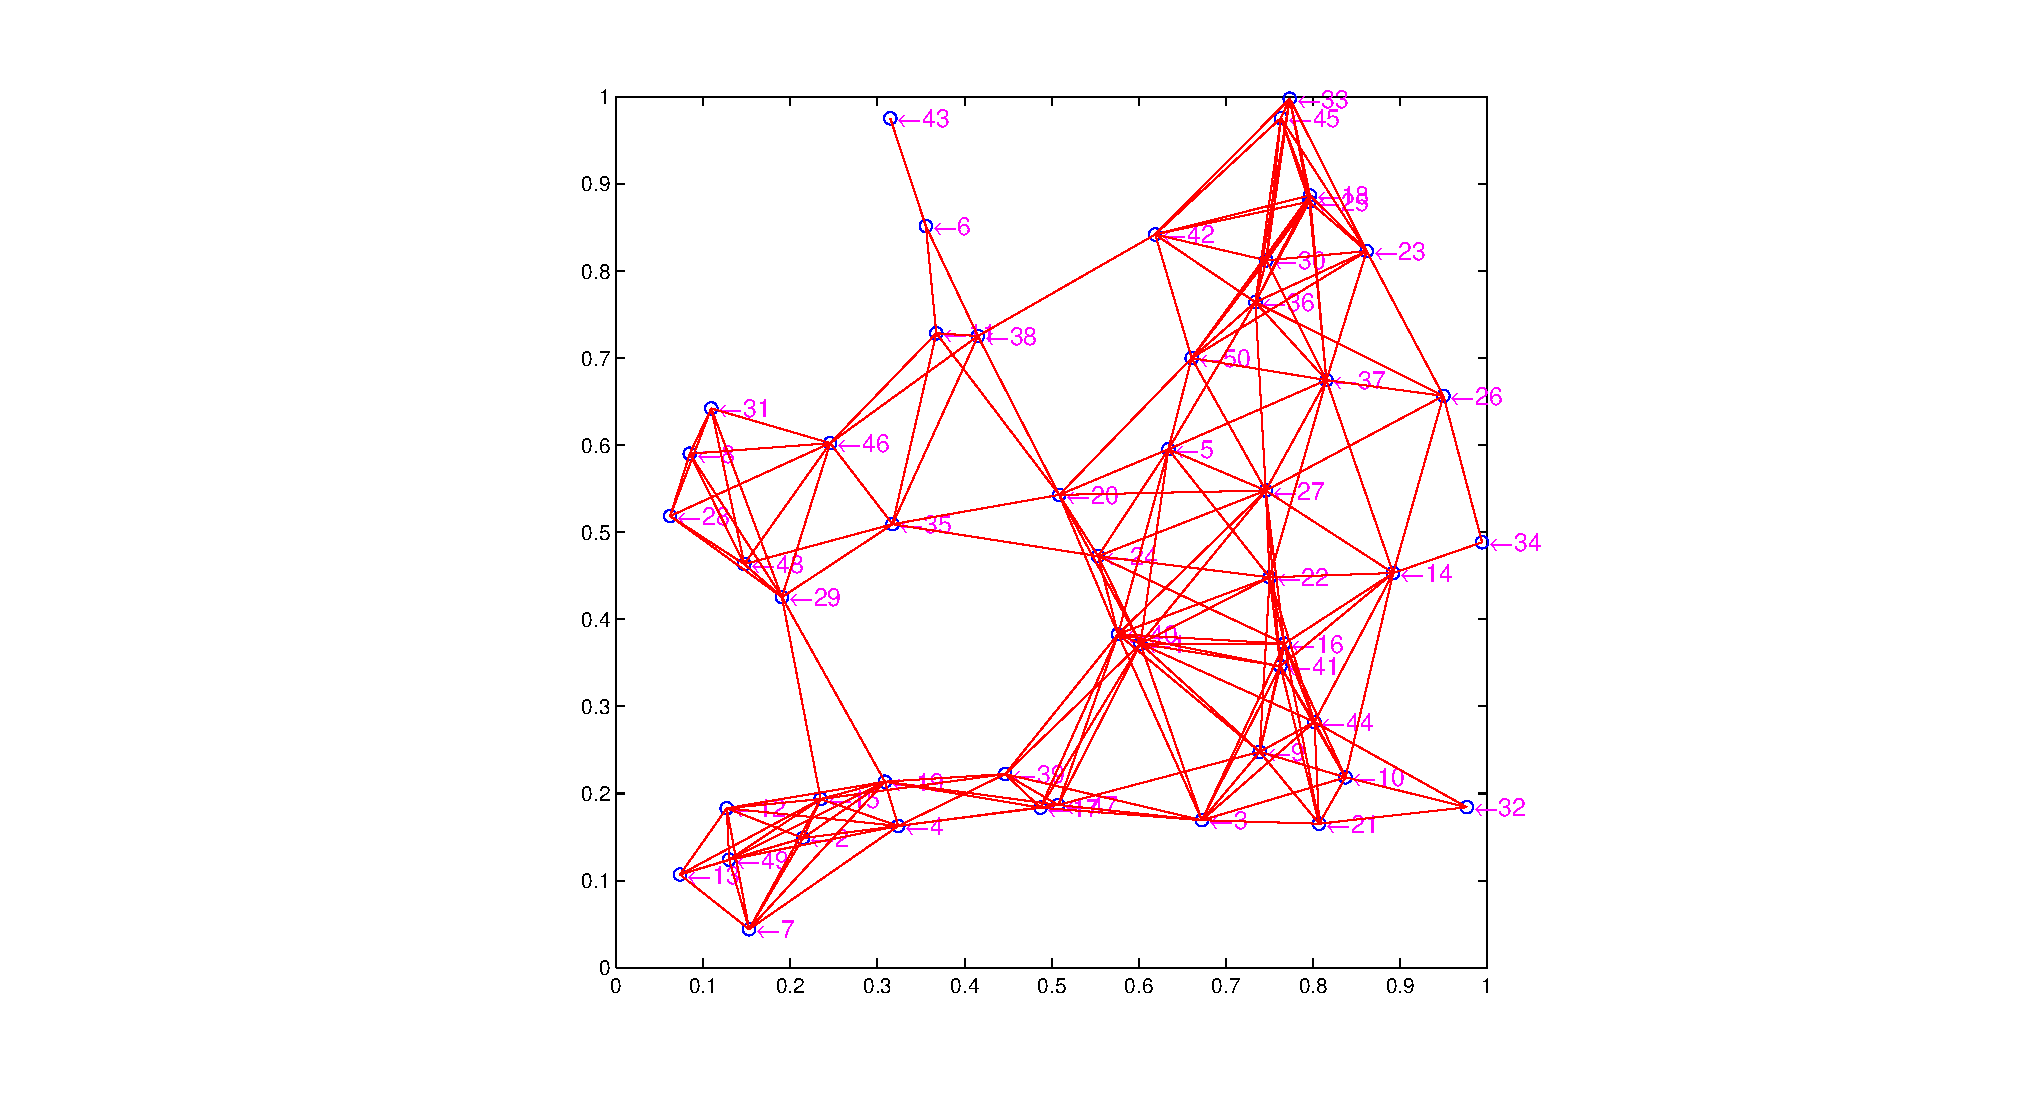
\includegraphics[width=7cm]{Graph/FirstYearReport/Lyx_v/images/Net50Edges200}

}\hfill{}\subfloat[\label{fig:Net-N16-R0,3}]{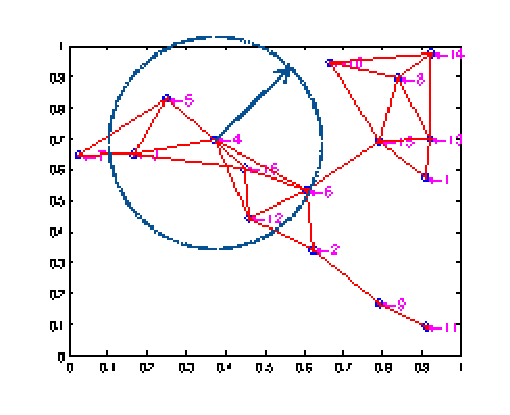
\includegraphics[width=7cm]{Graph/FirstYearReport/Lyx_v/images/Network_N16_R0,3}

}\hfill{}\caption{\label{fig:Random-Network}Randomly generated networks (a) 50 nodes
and 200 edges (b) 16 nodes and radius constrain $R=0.3$}
\end{figure}


There are some cases to generate the links between nodes.
\begin{casenv}
\item Consider the graph show in the Fig.\ref{fig:Net-N50-E200}, which
has 50 nodes and 200 edges.The number of nodes and edges are fixed;
50 nodes are randomly and uniformly distribute in the unit square;
a list that contains 200 shortest edges is created; Nodes are connected
if the edges belongs to the list. 
\item The network in Fig.\ref{fig:Net-N16-R0,3} is generating by connecting
any two nodes if their distance is less than the communication radius
constrain $R$. 
\end{casenv}

\subsubsection{Performance Comparison for Asymptotic DAC}

The figure.\ref{fig:DAC-SR-comp} shows the optimal spectral radius
for DAC algorithms with different communication radius constraints.
The performance for DAC algorithms with different orders are compared
by optimal spectral radius $\rho_{opt}=\mbox{\mbox{min}}\rho\left\{ \left(\mathbf{H}-\mathbf{J}\right)\right\} $,
which has the relationship with convergence rate given by $r_{opt}=-log\left(\rho_{opt}\right)$.
Y-axis is corresponding to the minimum spectral radius and x-axis
is corresponding to the radius constrain. For each instance of DAC
algorithm, the result is the minimum on the surface $\mbox{max}\{\left|\lambda_{i}\left(\mathbf{H-J}\right)\right|\}$
obtained by numerical searching. Each curve is the average of simulations
realized for 1000 instance of DAC initialized with random local value
vectors and random networks.

In another point of view, figure.\ref{fig:DAC MSE Compare} plots
the convergence behavior of mean square error of high-order DAC algorithms
together with first order DAC on random network. The MSE is defined
by 
\begin{equation}
MSE(k)=\frac{1}{n}\sum_{i=1}^{n}\left|x_{i}(k)-\bar{x}\right|^{2}.
\end{equation}
which Actually it is the Euclidean distance between current local
vector and the global average. shows the result when radius constrain
$R$ is $0.3$. In observing the gradient of curves, it is apparent
that higher-order DAC algorithm have larger convergence rate. However,
there are negligible improvement for the fourth order DAC compared
to the third order one. Furthermore, high-order DAC has a MSE overshoot
at the beginning. This phenomenon happens especially when communication
radius is small. Second order DAC algorithm does have a faster convergence
rate than first order algorithm as the slop of the curve is steeper.
But it become worse as it converge to error tolerance $10^{-6}$ more
later than the first order algorithm. Therefore, A hybrid algorithm
is proposed to overcome this disadvantage. Its step size and forgetting
factor are equal to the of first order DAC step size and second order
DAC forgetting factor respectively.

\begin{figure}
\hfill{}\subfloat[\label{fig:DAC-SR-comp} ]{\includegraphics[width=7cm,height=6.5cm]{\string"Graph/FirstYearReport/Lyx_v/images/Spectrum radius Compare_old_Ord1234\string".pdf}}\hfill{}\subfloat[\label{fig:DAC MSE Compare} ]{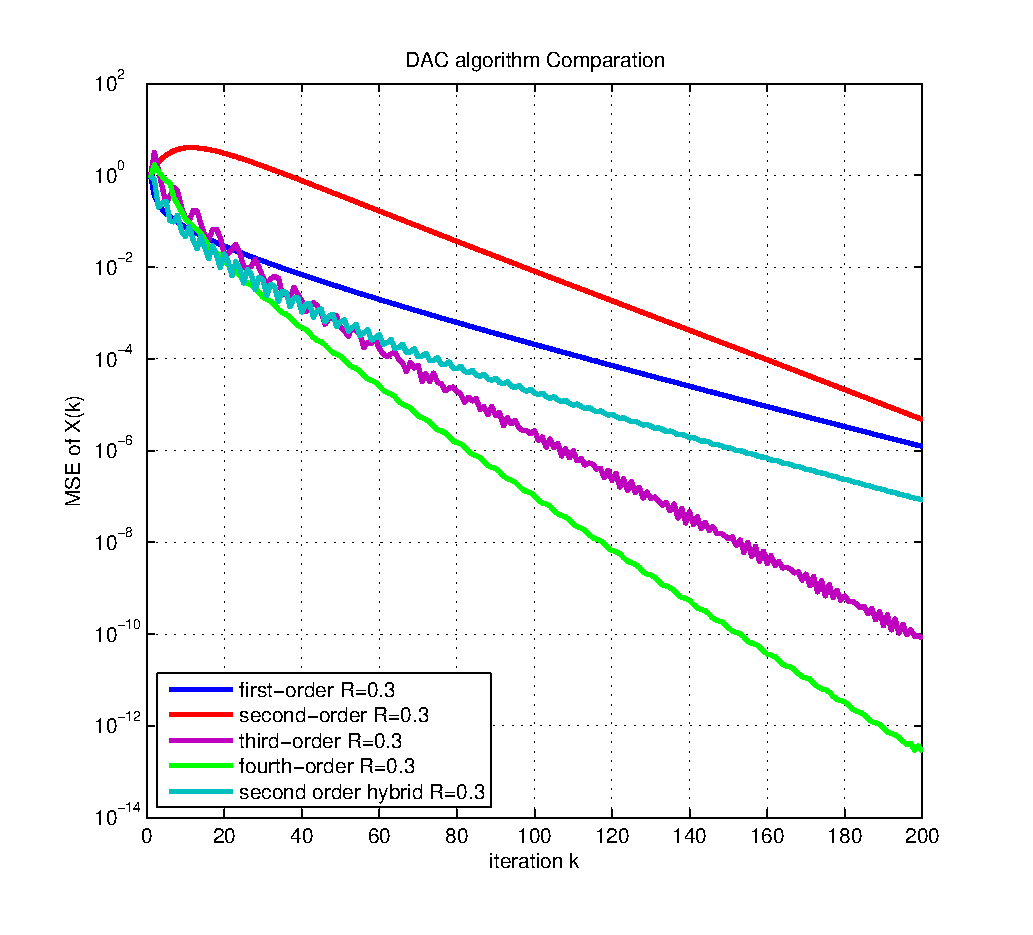
\includegraphics[width=7cm,height=6.5cm]{Graph/FirstYearReport/Lyx_v/images/DAC_Compr_ord1234&hybrid}

}\hfill{}

\caption{\label{fig:DAC-comparation}DAC algorithms comparison (a) compared
by spectral radius (b) compared by MSE}
\end{figure}



\include{\string"C2.5_Simple Finite-time_DCA\string"}


\section{Consensus Based Signal Processing}

Sensor networks have a variety of applications such as surveillance,
environment monitoring and collaborative signal processing. As the
advatages of reliability, survivability, and increased range of coverage,
there is an increasing interest in employing multiple distributed
sensors for these applications \cite{Chair1986}. A fundamental problem
in sensor network is to process spatially distributed information
using a scalable algorithm \cite{Olfati-Saber2005a}. 

Generally, there are two options for multiple sensors signal processing:
First option is centralized signal processing. This requires the network
contains a fusion center, and all sensor's information being transmuted
to the central processor. 

The Second option is distributed signal processing. Distributed average
consensus (DAC) algorithm is a tool for distributed information processing.
It has received significant attention recently because of its robustness
and simplicity. In this section, we will introduce two distributed
signal processing methods based on consensus algorithm.


\subsection{Data Fusion and Decision Making(todo check times 2)}

In this section, we will consider a distributed detection problem
in wireless sensor network without the fusion center. A consensus
based approach of distributed data fusion and decision making is introduced.

In centralized data fusion and decision making, a hypothesis test
based on the ML, MAP or Bayesian decision rule will be carried out
at the a fusion center.  Therefore, we intend to carry out the hypothesis
test in a distributed manner. 

Considering a binary hypothesis testing problem with the following
two hypotheses
\begin{enumerate}
\item H0: target is absent
\item H1: target is present.
\end{enumerate}
Suppose each sensor acquires a scale value from its sensoring area,
its signal has the following form

\begin{equation}
x_{l}=\begin{cases}
\mu_{l,0}+n_{l} & \mbox{if no target presents}\\
\mu_{l,1}+n_{l} & \mbox{if target presents}
\end{cases}
\end{equation}
where $\mu_{l,m}$ is the mean value of $x_{l}$ depending on hypothesis
$m$ and $n_{l}$ is the noise of $x_{l}$. The prior probability
of these two hypotheses is denoted by $P\left(H_{m}\right)=P_{m},m=1,2$.
The case when each sensor acquires a vector of unknown parameters
is discussed in \cite{Xiao2005}, where a more sophisticated data
fusion scheme is proposed.   

To make a declaration whether the target presents or not, based on
classical hypothesis test theory, the global log likelihood ratio
(G-LLR ) test is given by 

\begin{equation}
LLR(x_{1},...,x_{L})=\log\frac{f\left(x_{1},...,x_{L}|H_{1}\right)}{f\left(x_{1},...,x_{L}|H_{0}\right)}\underset{H_{0}}{\overset{H_{1}}{\gtrless}\log}\frac{P\left(H_{o}\right)}{P\left(H_{1}\right)}\label{eq:G-LLR define}
\end{equation}
where $f\left(x_{1},...,x_{L}|H_{m}\right)$ is the likelihood function
of hypothesis $H_{m}$.

Usually  we can assume the sensor detections are independent from
one to another. Therefore, we have $f\left(x_{1},...,x_{L}|H_{m}\right)=f\left(x_{1}|H_{1}\right)\cdot\ldots\cdot f\left(x_{L}|H_{1}\right)$
and 

\begin{eqnarray}
LLR(\mathbf{x}) & = & \log\frac{f\left(x_{1}|H_{1}\right)\cdot\ldots\cdot f\left(x_{L}|H_{1}\right)}{f\left(x_{1}|H_{0}\right)\cdot\ldots\cdot f\left(x_{L}|H_{0}\right)}=\sum_{i=1}^{L}LLR\left(x_{i}\right)\label{eq:Sum_L_LLR}
\end{eqnarray}


According to Eq.\eqref{Sum_L_LLR}, the G-LLR is the sum of local
log likelihood ratio (L-LLR) and can be calculated by distributed
average consensus (DAC) algorithm. This is implemented by the following
steps: First, each sensor node $i$ only calculate its L-LLR individually
based on $x_{i}$; Then, all the sensors update their L-LLR in the
DAC iteration until they converge to a common value; Finally, once
the algorithm converges, the G-LLR is obtained by multiply the average
value with the number of sensors in the network.


\subsubsection*{Generalization of LLR Calculation }

In this section, we will generalize the conditions step by step and
drive some expressions to show how to calculate G-LLR with DAC algorithms. 

First we assume the noises in sensor's signals are not independent
from one to another. The noises can be denoted by the joint Gaussian
white noise. 

Let the sensors observation, the joint Gaussian white noises and the
mean of sensor observation in a vector form given by 
\[
\mathbf{x}=\left[x_{1},\ldots,x_{L}\right]^{\mathrm{T}}
\]


\[
\mathbf{n}=\left[n_{1},\ldots,n_{L}\right]^{\mathrm{T}}\sim\mathcal{N}\left(0,\Sigma\right)
\]


\begin{equation}
\mathbf{u}_{m}=\left[\mu_{1,m},\ldots,\mu_{L,m}\right]^{\mathrm{T}},\; m=0,1.
\end{equation}
Since $\mathbf{n}\sim\mathcal{N}\left(0,\Sigma\right)$, the likelihood
function is a joint Gaussian function $f\left(x_{1},...,x_{L}|H_{m}\right)=\frac{1}{\left(2\pi\right)^{L/2}\left|\Sigma\right|^{\frac{1}{2}}}\exp\left(-\frac{1}{2}\left(\mathbf{x}-\mathbf{u}_{m}\right)^{T}\Sigma^{-1}\left(\mathbf{x}-\mathbf{u}_{m}\right)\right)$,
the G-LLR becomes 
\begin{eqnarray}
LLR(\mathbf{x}) & = & \left(\mathbf{u}_{1}^{\mathrm{T}}-\mathbf{u}_{0}^{\mathrm{T}}\right)\mathbf{\Sigma}^{-1}\mathbf{x}+\frac{1}{2}\left(\mathbf{u}_{0}^{\mathrm{T}}\mathbf{\Sigma}^{-1}\mathbf{u}_{0}-\mathbf{u}_{1}^{\mathrm{T}}\mathbf{\Sigma}^{-1}\mathbf{u}_{1}\right)\label{eq:wighted_sum_LLR}\\
 & = & \sum_{l=1}^{L}w_{l}x_{l}+C\nonumber 
\end{eqnarray}
where $w_{l}$ is the $l^{th}$ component of $\left(\mathbf{u}_{1}^{\mathrm{T}}-\mathbf{u}_{0}^{\mathrm{T}}\right)\mathbf{\Sigma}^{-1}$,
$C$ is the last term the equation. Eq. \eqref{wighted_sum_LLR} means
the G-LLR can be a weighted sum of sensor's observation. 

Provided that each sensor knows the weight $w_{l}$ and $C$, the
G-LLR is equal to the weighted sum of sensor's observation plus $C$.
Actually, the constant $C$ changes the threshold of the hypothesis
testing and can be subtract from both side of the equation. Therefore,
we modify the hypothesis testing into 
\[
\sum_{l=1}^{L}w_{l}x_{l}\underset{H_{0}}{\overset{H_{1}}{\gtrless}}\frac{P\left(H_{o}\right)}{P\left(H_{1}\right)}-C
\]
where the average values $\mbox{Avg}\left(w_{l}x_{l}\right)$ is obtained
by distributed average consensus (DAC) algorithm. Then the average
is multiplied with the number of sensors in the network to get $\sum_{l=1}^{L}w_{l}x_{l}$.


In the section of cloud detection \secref{Distributed_Cloud_De},
more generalized conditions of calculating the G-LLR is discussed
and more results about applying DAC algorithm will be presented. The
sensor signals will be correlated and mixed with joint Gaussian white
noises. In addition, the noises are not only correlated but also depends
on the existence of target. 


\subsection{Network Information Flooding(todo check times 0)}

The conventional information flooding is actually done by copying
information to all other nodes. Each node maintains a table of the
of all nodes values in the network, initialized with its own value,
and exchanges the tables of their own with those from their neighbors
in each step. After a certain number of time steps which is equal
to the diameter of the network, each node will obtain values of all
nodes. distributed averaging can also be implemented by this way. 

However, copying information and forwarding to all other nodes takes
too much resources for the networks. If a networks has $n$ nodes,
the conventional flooding will needs at least $\left(n-1\right)$
copies for each piece of information. And this estimation doesn't
considering the cost in transmitting the information to the destination.

We intend to develop an algorithm to accomplish the information flooding,
but didn't copy all the information to other nodes, so that the communication
cost can be dramatically reduced. However, The difficulties of this
kinds of distributed signal processing is that any individual node
only know partial information on the whole network. And information
exchange only allowed between neighbors. 

Based on the FT-DAC algorithm we introduced in the section \ref{sub:Finite-time-Consensus-on},
each node could decompose the local value vector by a linear combination
of eigenvalues and eigenvectors and can calculate the coefficients
before each term. Actually, with some signal processing techniques,
there are more information in the local values sequence that each
node can extract. These may also be applied to wireless sensor networks
as they could be carried out distributively. 

Therefore, in this section we propose a novel network information
flooding technique based on consensus algorithm. It doesn't require
copying information for so many time, instead, it transmit information
by broadcasting. The advantage of this method is that it can save
the costs in copying and transmitting information. 

Suppose the network weight matrix $W$ satisfies the same condition
\ref{eq:convege condition W}. Recall the initial local value decomposition
given by

\begin{equation}
\mathbf{x}\left(0\right)=\sum_{j=1}^{n}\alpha_{j}\mathbf{e}_{j}\label{eq:initial vector decompose-1}
\end{equation}
which shows that the initial local value vector can be defined by
a set of coefficients and a new basis defined by the eigenvectors.\textbf{
}In addition, the eigenvectors $\mathbf{e}_{i}$ are only depends
on the weight matrix. Therefore, once the coefficients $\alpha_{i}$
and weight matrix are available, the initial values vector $\mathbf{x}\left(0\right)$
can be calculated. It is possible to exchange information between
nodes in the network without copying information to all other nodes.

To show how this method can be carried out distributively, let the
sample vector $\mathbf{y}_{i}(k,d)\in R^{d}$ is defined by the history
of $x_{i}(k)$ 

\begin{equation}
\mathbf{y}_{i}(k,d)=\left[x_{i}(k),x_{i}(k-1),\ldots x_{i}(k-d+1)\right]^{\mathrm{T}}
\end{equation}
and the coefficients vector $\mathbf{a}=\left[\alpha_{1},\alpha_{2},\ldots,\alpha_{n}\right]^{T}$.
If we involve the eigenvectors and redefine the \eqref{Vander_beta}
by 
\begin{equation}
\mathbf{y}_{i}(k,d)=\mathbf{V}_{i}(k,d)diag\left(\left[\mathbf{e}_{1}^{T}\mathbf{u}_{i},\mathbf{e}_{2}^{T}\mathbf{u}_{i},\ldots,\mathbf{e}_{n}^{T}\mathbf{u}_{i}\right]\right)\mathbf{a}\label{eq:Vander_Eigen_ith_Alpha}
\end{equation}
where $\mathbf{u}_{i}$ is the unit vector with all zero except the
$i^{th}$ component is one, $\mathbf{e}_{j}^{T}\mathbf{u}_{i}$ means
the $i^{th}$ component of $\mathbf{e}_{j}$. Solving the above equation
will obtain the coefficients $\alpha_{j}$. 

The consensus based information flooding is ideally suitable for time-invariant
network. Because this method requires a node know all the eigenvectors
and eigenvalues of the network before it can estimate initial values
of other nodes. It can be initialized by all flooding weight coefficients
to all nodes in the network. However, instead of flooding a table
of local values, flooding the weight matrix is only performed at the
stage initialization for one time. The proposed method could have
lower cost both in computation and communication, if the topology
changes at a very low frequency.



\section{Graph Theory and Matrix Theory Review }

In this section, some basic concepts of the graph theory and matrix
theory will be introduced. They are used in the analysis of convergence
or performance of consensus algorithm. Because consensus algorithm
actually relates to a matrix iteration algorithm, it is necessary
to introduce some of these theorems. For full information about matrix
theory, see \cite{Varga2010}, and the work \cite{Russell1994} states
more details about Laplacian matrix. However, some useful properties
of Laplacian matrix will to be introduced here. 

Let ${\cal G}=\left({\cal V},{\cal E},{\cal A}\right)$ be a graph
with $n$ nodes. The in-degree and out-degree of node $i$ are defined
by:

\begin{equation}
D_{in}\left(i\right)=\sum_{i=1}^{n}a_{i,j}
\end{equation}
\begin{equation}
D_{out}\left(i\right)=\sum_{j=1}^{n}a_{i,j}
\end{equation}
where $a_{i,j}$ is the elements of matrix ${\cal A}$. This definition
states that in-degree of node $i$ is the $i^{th}$ column sum of
matrix ${\cal A}$ and the out-degree of node $i$ is the $i^{th}$
row sum of matrix ${\cal A}.$ And the graph Laplacian matrix ${\cal L}$
induced by the ${\cal G}$ is the same as defined before, see \ref{eq:Graph Laplacian def.}.
In addition, we can find the relationship of ${\cal L}$ and ${\cal A}$.
\begin{equation}
{\cal L}=\Delta-{\cal A}
\end{equation}
 where $\Delta$ is a diagonal matrix $\Delta=\left[\Delta_{i,j}\right]$,
$\Delta_{i,j}=0$ for all $i\neq j$ and $\Delta_{ii}=D_{out}\left(i\right)$.

Note that we assume the diagonal elements $a_{i,i}$ of matrix ${\cal A}$
equal to zero for all $i$. Thus, the Laplacian matrix is only dependent
on the off-diagonal elements of ${\cal A}$. Moreover, if we assume
matrix ${\cal A}$ is non-negative, we can benefit from the properties
of non-negative matrix, and use them in optimization of convergence
rate of consensus algorithm.


\subsection{Irreducibility and Strong Connected Graph.}

For an undirected graph, the consensus $\mathbf{x}^{*}$ can be achieved
if and only if the graph is connected. (Note that the consensus is
a stable state of the system dynamic. For the average consensus problem
the consensus state is a state where all the network node converge
to the global average.) But for the directed graph, this condition
of achieving consensus becomes into if and only if the graph is strongly
connected. 

A directed graph is strongly connected if and only if for any two
distinct nodes $i$ and $j$, there exists a path that follows the
direction of the edges and connects $i$ and $j$ on the digraph. 
\begin{defn}
\label{Def.Irreducebility}for $n>1$, an $n\times n$ matrix $A\in R^{n\times n}$
is reducible if there exists an $n\times n$ permutation matrix $P$
such that $PAP^{T}$ is in block upper triangular form. 
\begin{equation}
PAP^{T}=\left[\begin{array}{cc}
A_{1,1} & A_{1,2,}\\
O & A_{2,2}
\end{array}\right]
\end{equation}
where $A_{1,1}$ is an $r\times r$ submatrix and $A_{2,2}$ is an
$\left(n-r\right)\times\left(n-r\right)$ submatrix, and $O$ is an
null matrix, $1\leq r<n$. If no such a permutation matrix exists,
the matrix $A$ is irreducible. If $n=1$, then $A$ is reducible
if $A=0$, and irreducible otherwise. 
\end{defn}
The relationship of the irreducible property of matrix $A$ and the
strong connected property of directed graph ${\cal G}\left(A\right)$
is stated by the following theorem.
\begin{thm}
An $n\times n$ complex matrix $A\in C^{n\times n}$ is irreducible
if and only if its directed graph ${\cal G}\left(A\right)$ is strongly
connected. \cite{Varga2010}
\end{thm}
The proof of this theorem is obvious. If a graph is strongly connected,
all the off diagonal elements of graph matrix $A$ cannot be vanished
by matrix permutation. Therefore, matrix $A$ doesn't exists the block
upper triangular form as given in Def. \ref{Def.Irreducebility}. 


\subsection{Spectral radius of a matrix}

Spectral radius of a matrix is one of the basic concepts in the matrix
iteration theory. It is defined by the largest eigenvalue of the matrix.
The matrix iteration is very useful in many applications, denoted
by $A,A^{2},A^{3},\ldots$. The power sequence is said to be convergent,
if and only if $\lim_{k\to\infty}A^{k}=O$, where $O$ is a zero matrix
with all zero entries. The following theorem states that the convergent
property is strongly connected with the spectral radius. 
\begin{thm}
\label{thm:Convergent <=00003D> p(A)<1} if $A\in C^{n\times n}$
is an $n\times n$ complex matrix, then $A$ is convergent if and
only if $\rho\left(A\right)<1.$\end{thm}
\begin{proof}
The proof uses the Jordan form of a matrix. For any matrix $A\in C^{n\times n}$,
there exists a nonsingular $n\times n$ matrix $T$, such that $A$
reduces into the Jordan normal form 
\begin{equation}
T^{-1}AT=J=\left[\begin{array}{cccc}
J_{1} &  &  & O\\
 & J_{2}\\
O &  & \ddots & J_{m}
\end{array}\right]
\end{equation}
 where each Jordan block $J_{i}$ is an $r_{i}\times r_{i}$ submatrix
in the form 
\begin{equation}
J_{i}=\left[\begin{array}{ccccc}
\lambda_{i} & 1\\
 & \lambda_{i} & 1\\
 &  & \lambda_{i} & \ddots\\
 &  &  & \ddots & 1\\
 &  &  &  & \lambda_{i}
\end{array}\right]
\end{equation}
Thus, the matrix $J$ and $A$ are similar and have the same eigenvalues
$\lambda_{i},i=1,\ldots m$

A direct computation of the power iteration of matrix $A$ will give
us the following equation
\[
A^{k}=TJ^{k}T^{-1}=T\left[\begin{array}{cccc}
J_{1}^{k} &  &  & O\\
 & J_{2}^{k}\\
O &  & \ddots & J_{m}^{k}
\end{array}\right]T^{-1}
\]
because the property of Jordan block, the power of each Jordan block
will have the form
\[
J_{i}^{2}=\left[\begin{array}{ccccc}
\lambda_{i}^{2} & 2\lambda_{i} & 1\\
 & \lambda_{i}^{2} & 2\lambda_{i} & \ddots\\
 &  & \lambda_{i}^{2} & \ddots & 1\\
 &  &  & \ddots & 2\lambda_{i}\\
 &  &  &  & \lambda_{i}^{2}
\end{array}\right],\mbox{if }r_{i}\geq3
\]
 and more generally, let $J_{i}^{k}=\left[c_{m,n}\left(i,k\right)\right]$,
$1\leq m$, $n\leq r_{i}$, and it has 
\[
c_{m,n}\left(i,k\right)=\begin{cases}
0 & n<m\\
\left(\begin{array}{c}
k\\
n-m
\end{array}\right)\lambda_{i}^{k-n+m} & m\leq n\leq\min\left(r_{i},k+m\right)\\
0 & k+m<n<r_{i}
\end{cases}
\]
 Since $\rho\left(A\right)<1$, and matrix $J$ share the same eigenvalues
with $A$, $\left|\lambda_{i}\right|<1$. This lead to $\lim_{k\to\infty}c_{m,n}\left(i,k\right)=0,\:\mbox{for all }1\leq m\leq r_{i},1\leq n\leq r_{i}$,
so that the each Jordan block is convergent. Therefore, the matrix
iteration $A^{k}=TJ^{k}T^{-1}$ is also convergent. This completes
the proof. 
\end{proof}
We give the proof of \prettyref{thm:Convergent <=00003D> p(A)<1}
here as it will be very useful in the proof of an convergence conditions
theorem for distributed consensus algorithm, see \prettyref{sub:DT-First-Order-DAC}.
At the same time, the Jordan normal form weight matrix $W^{k}=TJ^{k}T^{-1}$
gives the local value vector $\mathbf{x}\left(k\right)=W^{k}\mathbf{x}\left(0\right)$
another expression in terms of eigenvalues and eigenvectors, which
reflects the basic ideas of the finite-time consensus algorithm. This
will be introduced in \prettyref{sec:Finite-Time-Distributed-Consensu}. 


\subsubsection{Gerschgorin's theorem}

The calculation of eigenvalues a matrix $A$ involves determination
of the matrix $\lambda I-A$ and solving a high order polynomial equation.
In some situations, for example, when the matrix dimension is very
large, it is very difficult to determine the spectral radius precisely.
However, the following theorem of Gerschgorin provides an upper bound
of the spectral radius \cite{Horn1990}.
\begin{thm}
Let $A=\left(a_{i,j}\right)$ be an arbitrary $n\times n$ matrix.
Denote the 
\begin{equation}
d_{i}=\sum_{j=1,j\neq i}^{n}\left|a_{i,j}\right|
\end{equation}
then all the eigenvalues of matrix $A$ are lie in the union of the
disks.
\begin{equation}
\left|z-a_{i,i}\right|\leq d_{i},\ 1\leq i\leq n.
\end{equation}

\end{thm}
The above theorem is well-known, so the proof is omit here. But the
theorem immediately give the result of
\begin{cor}
\label{cor:Upper Bound of p(A)}Let $A=\left(a_{i,j}\right)$ be an
arbitrary $n\times n$ matrix, and 
\begin{equation}
v=\max_{1\leq i\leq n}\sum_{j=1}^{n}\left|a_{i,j}\right|
\end{equation}
then we have $\rho\left(A\right)\leq v$. 
\end{cor}
Therefore, the maximum of the row sums of the modular of the entries
of matrix $A$ provides a upper bound for spectral radius $\rho\left(A\right)$.
Since $A$ and $A^{T}$ have the same eigenvalues, applying the \ref{cor:Upper Bound of p(A)}
to $A^{T}$ will lead to 
\begin{cor}
Let $A=\left(a_{i,j}\right)$ be an arbitrary $n\times n$ matrix,
and 
\begin{equation}
v'=\max_{1\leq j\leq n}\sum_{i=1}^{n}\left|a_{i,j}\right|
\end{equation}
then we have $\rho\left(A\right)\leq v'$.
\end{cor}
As both the row sum and column sum of the modular of the entries of
matrix can provide the upper bound for $\rho\left(A\right)$, the
minimum of $v$ and $v'$ gives the better upper bound. 



Just as we assume before, the adjacent matrix ${\cal A}$ of the graph
${\cal G}$ is non-negative, which means all elements are non-negative.
Then, the induced graph Laplacian matrix will have the following result
using the Gerschgorin's theorem. 




\subsubsection{Perron-Frobenius Theorem}

The Perron-Frobenius theorem states that if matrix $A$ is nonnegative
and irreducible which means the digraph of matrix A is strongly connected,
the spectral radius $\rho(A)$ is equal to a simple eigenvalue of
$A$ associated with a positive eigenvector \cite{Piziak2007}. The
details of Perron-Frobenius is as follows.
\begin{thm}
\label{thm:Perron-Frobenius thm.} Let $A$ be an $n\times n$ and
irreducible matrix with non-negative and real numbers as its entries.
Then, \end{thm}
\begin{enumerate}
\item $A$ has a positive real eigenvalue equal to its spectral radius $\rho\left(A\right)$.
\item $\rho\left(A\right)$ is a simple eigenvalue of $A$.
\item To the eigenvalue $\rho\left(A\right)$, the corresponding eigenvector
is positive, i.e. $\mathbf{x}>\mathbf{0}$.
\item $\rho\left(A\right)$ increases if any entry of $A$ increases.
\end{enumerate}
Recall the problem of finding the bounds for the spectral radius,
the Perron-Frobenius theorem provides the nontrivial lower-bound of
$\rho\left(A\right)$. In the \prettyref{cor:Upper Bound of p(A)},
the nontrivial upper bound of $\rho\left(A\right)$ is found. Together
with these two results, we can have a conclusion of the spectral radius
of a non-negative and irreducible matrix given in the following.
\begin{lem}
If $A=\left[a_{i,j}\right]$ is an $n\times n$ non-negative and irreducible
matrix, then either 
\begin{equation}
\sum_{j=1}^{n}a_{i,j}=\rho\left(A\right),\mbox{for all }1\leq i\leq n,
\end{equation}
or 
\begin{equation}
\min_{1\leq i\leq n}\left(\sum_{j=1}^{n}a_{i,j}\right)<\rho\left(A\right)<\max_{1\leq i\leq n}\left(\sum_{j=1}^{n}a_{i,j}\right).
\end{equation}
\end{lem}
\begin{thm}
Let $A=\left[a_{i,j}\right]$ be an $n\times n$ non-negative and
irreducible matrix, for any $\mathbf{x}>\mathbf{0}$, either
\begin{equation}
\min_{1\leq i\leq n}\left(\frac{\sum_{j=1}^{n}a_{i,j}x_{j}}{x_{i}}\right)<\rho\left(A\right)<\max_{1\leq i\leq n}\left(\frac{\sum_{j=1}^{n}a_{i,j}x_{j}}{x_{i}}\right)
\end{equation}
or 
\begin{equation}
\frac{\sum_{j=1}^{n}a_{i,j}x_{j}}{x_{i}}=\rho\left(A\right),\ \mbox{for all }1\leq i\leq n.
\end{equation}
Moreover,
\begin{equation}
\max_{\mathbf{x}\in P}\min_{1\leq i\leq n}\left(\frac{\sum_{j=1}^{n}a_{i,j}x_{j}}{x_{i}}\right)=\rho\left(A\right)=\min_{\mathbf{x}\in P}\max_{1\leq i\leq n}\left(\frac{\sum_{j=1}^{n}a_{i,j}x_{j}}{x_{i}}\right)
\end{equation}

\end{thm}
The equality is valid if we choose the $\mathbf{x}$ equal to the
positive eigenvector $e>0$ corresponding to the eigenvalue $\rho\left(A\right)$.
The method shown above will be applicable, because it provides us
both the upper bounds and lower bounds for the spectral radius of
a non-negative and irreducible matrix, by a simple algorithm without
calculating the determination of $\lambda I-A$. 




\subsection{Diagonalizable matrix \& Symmetric matrix}

The Jordan normal form of weight matrix $W^{k}=TJ^{k}T^{-1}$ gives
the local value vector $\mathbf{x}\left(k\right)=W^{k}\mathbf{x}\left(0\right)$
an analitical expression in terms of eigenvalues and eigenvectors.
Moreover, if the matrix $W$ is symmetric, the expressions of $\mathbf{x}\left(k\right)$
can be simplified. Then, algorithms such as the finite-time consensus,
can be implemented more easily. In addition, under the the assumption
of symmetric weight matrices, the optimal weight matrix which has
the fastest convergence rate can be found through a semi-definite
problem. \cite{Li2010}. 
\begin{defn}
A matrix $A$ is diagonalized, if and only if there exist a nonsigular
matrix $T$, which reduce $A$ into the form 
\[
T^{-1}AT=\mbox{diag}\left(\lambda_{1},\lambda_{2},\ldots,\lambda_{n}\right)
\]

\end{defn}
Generally, a matrix are diagonalized by an unitary matrix if and only
if it is normal. Normal matrix $A$ means it satisfies $A^{H}A=AA^{H}$.
Let $\lambda_{1},\lambda_{2},\ldots,\lambda_{n}$ be the eigenvalues
of $A$. There exists a unitary matrix $U$, which satisfies $U^{H}=U^{-1}$,
such that $U^{-1}AU=\mbox{diag}\left(\lambda_{1},\lambda_{2},\ldots,\lambda_{n}\right)$.
For real normal matrix $A$, if all of its eigenvalues are real, there
exists an orthogonal matrix $P,$ which has $P^{T}=P^{-1}$, reduces
the real matrix $A$ into diagonalized form $P^{-1}AP=\mbox{diag}\left(\lambda_{1},\lambda_{2},\ldots,\lambda_{n}\right)$. 

Specificlly, any real nonsigular symmetric matrix $A\in R^{n\times n}$
has $n$ linearly independent real eigenvectors. Moreover, these eigenvectors
can be chosen so that they are orthogonal to each other with modular
one. Thus, the real symmetric matrix can be decomposed by an orthogonal
matrix $P$, i.e. $A=P\Lambda P^{-1}$, where $\Lambda$ is a diagonal
matrix whose entries equal to the eigenvalues of $A$. Also the symmetric
matrix has all its eigenvalues algebra multiplicity equal to the gerometric
multiplicity, so all the Jordan block have size one.



\chapter{\label{sub:Finite-time-Consensus-on}Finite-time DAC on Generalized
Conditions }

(todo check 1)

It is shown in section \ref{sub:Find_Consensus_Value} that finite-time
DAC algorithm can calculate the consensus value by a linear combination
of local values in the past, if each node knows the network topology
(or eigenvalues of the weight matrix $W$). However, having knowledge
of the network topology in every node is a demanding assumption. Although
a distributed algorithm to calculate the linear combination has also
been introduced in \cite{Sundaram2007}, it requires several runs
of the consensus algorithm initialized with a set of linear independent
vectors. Alternatively, the original consensus algorithm can run many
instances in parallel with a set of independent initial values. However,
the data transmission at each iteration increases. Futhermore, this
method may not reliable to topology changes during the of multiple
re-initializations of original consensus algorithm. 

Here we propose a generalized finite-time DAC algorithm, which does
not require knowledge of network topology and re-initialization of
the original consensus algorithm for several times. In the future
research, the finite-time DAC algorithm probably will be generalized
to non-symmetrical network. Before introducing the algorithm, there
are too important linear filter need to be introduced, as the algorithm
is based on the properties of these filters. The first is the FIR
filter to estimate the consensus value which introduced in section
\ref{sub:Find_Consensus_Value}. The second is introduced in the next
section \ref{sec:Linear-Predictor-For}.


\section{\label{sec:Linear-Predictor-For}Linear Predictor For Local Value
(todo check times 1)}

In observing the convergence curve of each node's local value sequence,
we would come to the idea that the sequence must obeys some rule as
it converges. In section \ref{sub:Find_Consensus_Value}, it is shown
that local value vector can be decomposed in terms of eigenvalues
and eigenvectors. Based on this fact, a consensus value estimation
method by inverting the Vandermonde matrix  are proposed.

However, another important property of the FO-DCA need to be highlighted
in this section. To show this , we have the following theorem.
\begin{thm}
\label{thm:LV predictor a_i} For the DAC iteration $\mathbf{x}(k+1)=W\mathbf{x}(k)$
with $W$ satisfying the convergence condition in theorem \ref{thm:convergence condition}
, for any $k\geq m$ , where $m$ is a certain number, local value
\textup{$x_{i}\left(k\right)$} at node $v_{i}$ is equal to a linear
combination of local values of itself in $m$ previous time steps,
i.e. $x_{i}\left(k\right)=-a_{m-1}x_{i}\left(k-1\right)-\ldots-a_{1}x_{i}\left(k-m+1\right)-a_{0}x_{i}\left(k-m\right)$. \end{thm}
\begin{proof}
the minimal polynomial of $W$ is given by

\begin{eqnarray}
p(\lambda) & = & \prod_{i=1}^{r}\left(\lambda-\lambda_{i}\right)^{r_{i}}=0\nonumber \\
 & = & \lambda^{m}+a_{m-1}\lambda^{m-1}+\ldots+a_{1}\lambda+a_{0}\label{eq:polynomial of matrix W}
\end{eqnarray}
where $m=\sum_{i=1}^{r}r_{i}$. Since $p\left(W\right)=\mathbf{0}_{n\times n}$,
we have, 
\[
W^{m}+a_{m-1}W^{m-1}+\ldots+a_{1}W+a_{0}I=\mathbf{0}_{n\times n}
\]
multiplying both sides with $\mathbf{x}\left(0\right)$ we obtain
\begin{equation}
\mathbf{x}\left(k\right)+a_{m-1}\mathbf{x}\left(k-1\right)+\ldots+a_{0}\mathbf{x}\left(k-m\right)=\mathbf{0}_{n\times n}\label{eq:x(k+r) vector predictor}
\end{equation}
For any node $v_{i}\in{\cal V}$, its local value at time $k$ is
just the $i^{th}$ component of $\mathbf{x}\left(k\right)$. After
a little evolution, we have

\begin{equation}
x_{i}\left(k\right)=-a_{m-1}x_{i}\left(k-1\right)-\ldots-a_{0}x_{i}\left(k-m\right)\label{eq:x(k+r) predictor}
\end{equation}
In other words, $x_{i}\left(k\right)$ can be predicted by a FIR filter
given by $\left[-a_{r},-a_{r-1},\ldots,-a_{0}\right]$, if we pass
a number of consecutive local values in the past through that filter,
after the time index $k>m$. In addition, all the nodes in the network
can share the same coefficients, when the minimal polynomial of $W$
is not changed.\end{proof}
\begin{lem}
\label{lem:Sum-coef.=00003D1}The sum coefficients \textup{$\left\{ a_{j}\right\} =\left\{ a_{m-1},\ldots,a_{1},a_{0}\right\} $}
is equals to negative one, i.e. $\sum_{j=0}^{m-1}a_{j}=-1$\textup{. }\end{lem}
\begin{proof}
It is obvious when the iteration converges. Since Eq. \prettyref{eq:x(k+r) vector predictor}
satisfied as $k\to\infty$, we have $\bar{\mathbf{x}}+a_{m-1}\bar{\mathbf{x}}+\ldots+a_{1}\bar{\mathbf{x}}+a_{0}\bar{\mathbf{x}}=\mathbf{0}$.
Then, canceling the vector $\bar{\mathbf{x}}$ from the equation obtains
that the sum of all coefficients equals to negative one. 
\end{proof}
Given the local value vector sequence obtained by FO-DCA, one may
instantly comes to the idea of applying an adaptive filter algorithm
to estimate the set of coefficient. For example, LMS, LSL and Kalman
filter algorithms. One advantage of the adaptive filter algorithm
is that when the network topology is changed, the filter could adaptively
change its coefficient during the iteration. 


\subsection*{Find the Coefficients of Linear Predictor.}

After running FO-DAC algorithm for a number of step, node $v_{i}$
could list a number of equations by its available local values. Once
they are sufficient equations to construct a matrix, which is a Toeplitz
matrix, we can have a important result in the following.

Let  $T_{i}=T_{i}\left(k,D_{i}\right)\in\mathbb{R}^{D_{i}\times D_{i}}$
be a function at $v_{i}$ which outputs a Toeplitz matrix with size
$D_{i}$ with $x_{i}\left(k\right)$ as diagonal entries.

$T_{i}\left(k,D_{i}\right)=$ 
\begin{align}
\left[\begin{array}{cccc}
x_{i}\left(k\right) & x_{i}\left(k-1\right) & \ldots & x_{i}\left(k-D_{i}+1\right)\\
x_{i}\left(k+1\right) & x_{i}\left(k\right) & \cdots & x_{i}\left(k-D_{i}+2\right)\\
\vdots & \vdots & \ddots & \vdots\\
x_{i}\left(k+D_{i}-2\right) & x_{i}\left(k+D_{i}-3\right) & \cdots & x_{i}\left(k-2\right)\\
x_{i}\left(k+D_{i}-1\right) & x_{i}\left(k+D_{i}-2\right) & \cdots & x_{i}\left(k\right)
\end{array}\right]\label{eq:Toeplitz_i simple-1}
\end{align}
Similarly, Define the function $\mathbf{y}_{i}=\mathbf{y}_{i}\left(k,D_{i}\right)=\left[x_{i}\left(k+1\right),x_{i}\left(k+2\right),\ldots,x_{i}\left(k+D_{i}\right)\right]^{T}\in\mathbb{R}^{D_{i}}$
which outputs the local value history at $v_{i}$ from time $k+1$
to $k+D_{i}$.  Then, let $\mathbf{a}_{i}\left(D_{i}\right)=\left[a_{i,D_{i}-1},\ldots,a_{i,1},a_{i,0}\right]^{T}\in\mathbb{R}^{D_{i}}$
be a vector of length $D_{i}$ representing the coefficients in the
minimal polynomial calculated at $v_{i}$. Then, we have the solution
of these equations given by

\begin{equation}
\mathbf{a}_{i}\left(D_{i}\right)=-T_{i}^{-1}\left(k,D_{i}\right)\mathbf{y}_{i}\left(k,D_{i}\right)\label{eq:Toeplitz Eq.-2}
\end{equation}
The size of the Toeplitz block $D_{i}$, should be less or equal to
$m$ so that the Eq. \prettyref{eq:Toeplitz Eq.-2} have unique solution.
To solve Eq.\ref{eq:Toeplitz Eq.-2}, node $i$ need to have sufficient
local values.

Toeplitz matrix is a special type of matrix and can be inverted by
some algorithms in the polynomial time of order $D_{i}^{2}$, rather
than the order of $D_{i}^{3}$ in general case (for example by LU
decomposition), which is an enormous computational saving \cite{Prass2007}.
Levinson developed a recursive algorithm to solve the system quickly
if the Toeplitz matrix is symmetric. 

One interesting advantage of Levinson's method is it can also apply
to the case when weight matrix is non-symmetric. The fact that the
method can be generalized to the non-symmetric case is stated in the
texts \cite{Robinson2000}.  Therefore, We will invert this Toeplitz
matrix using Levinson's method. The proposed method  doesn't need
to be changed and can generalize to the non-symmetric weight matrix
case. 

It totally needs $2r+2$ local values and $2r+1$ iterations to construct
the Toeplitz matrix and Eq.\ref{eq:Toeplitz Eq.-2}, but all the local
value can be obtained from one instance of FO-DCA. In contract, the
the original finite-time consensus algorithm in \cite{Sundaram2007}
requires $r$ iterations of FO-DCA for each instance, and totally
$r$ instances. Therefore, the proposed method has some improvement
to the original finite-time consensus algorithm. 

In the next section \ref{sub:Convert-Linear-Predictor }, we will
show how to obtain the consensus finding filter by linear predictor
coefficients.


\section{\label{sub:Convert-Linear-Predictor }Convert Linear Predictor To
Consensus Finding Filter(todo check times 0)}

Once there are sufficient local values, node $i$ can solve the equation
and obtain the set of coefficients \textbf{$\mathbf{a}$} and construct
the polynomial 
\[
p(\lambda)=\lambda^{m}+a_{m-1}\lambda^{m-1}+\ldots+a_{1}\lambda+a_{0}
\]


If matrix $W$ satisfies the condition in \prettyref{thm:convergence condition}
there is a simple eigenvalue equals to one. As shown in section \ref{sub:Find_Consensus_Value},
the consensus finding filter is given by the row of inverse of Vandermonde's
matrix which corresponding to an eigenvalue equals to one. Without
loss of generality, let the first eigenvalue $\lambda_{1}=1$. Thus,
the consensus finding filter is given by the first row of the inverse
of Vandermonde's Matrix.

Examining the the Lagrange's polynomial interpolation formula \prettyref{eq:Lagrange's polynomial}
we can rewrite the consensus finding filter in terms of $a_{k}$. 

To make the expression simple, we may define another polynomial (Also
see Eq.\prettyref{eq:intermindia polynomial})

\[
q\left(\lambda\right)=\frac{p\left(\lambda\right)}{\lambda-1}=c_{m}\lambda^{m-1}+c_{m-1}\lambda^{m-2}+\ldots+c_{2}\lambda+c_{1}
\]
where $c_{k}=1+\sum_{j=k+1}^{m}a_{j}$. The consensus finding filter
can be given by the coefficient in $q\left(\lambda\right)$. 
\begin{equation}
\mathbf{h}=\frac{\left[c_{m},c_{m-1},\ldots,c_{2}\right]}{\sum_{k=1}^{m}c_{k}}\label{eq:Consensus Filter by polynomial}
\end{equation}
This indicates the possibility of using the adaptive filter to estimate
the consensus value after a certain number of iterations. 

One interesting property of the consensus finding filter is that it
can be found by this method when the weight matrix is non-symmetric.
It can be demonstrated by finding the inverse of a confluent Vandermonde
matrix. In examining the expression of the inverse of confluent Vandermonde
matrix, we note that the row corresponding to the unity eigenvalue,
can actually the coefficients of a consensus finding filter. The the
length of the filter is not required to be the same. It may be not
equal to the number of distinct and nonzero eigenvalues $m$, but
equal to the sum of all orders in minimal polynomial of weight matrix
$\sum_{i=1}^{m}r_{i}$. However, the relationship of local value predictor
and consensus finding filter still holds. 


\section{Simulation\label{sub:Numerical-Simulation}}

\begin{figure}
\hfill{}\includegraphics{\string"Graph/Report_DAC/Net_Weight/graph with 8 nodes and 17 edges\string".pdf}\hfill{}\hfill{}\caption{\label{fig:Graph in Xiao'paper}Graph with optimal weights which maximize
convergence rate }
\end{figure}


Consider the graph from \cite{Xiao2004}, the weight matrix \textbf{$W$}
corresponding to this graph is symmetric and has eigenvalues $\lambda(W)=\{1,0.6,0.4,0,0,0,-0.4,-0.6\}$.
The time index $k$ can be chosen large enough so that there are surfficient
number of local values to estimate the filter coefficients.  For example,
there are 5 distinct and nonzero eigenvalues of \textbf{$W$}, so
we choose the time index $k=5$ and $d=5$ which is the minimum filter
length.

 Based on Eq.\ref{eq:Consensus Filter by polynomial}  the consensus
finding filter is given by

\[
\mathbf{h}=\left[1.8601,\;0,\;-0.9673,\;0,\;0.1071\right]^{\mathrm{T}}
\]


\begin{figure}
\hfill{}\includegraphics[width=8cm]{\string"Graph/Report_DAC/MSE/MSE_Filter vs FODAC\string".pdf}\hfill{}

\caption{\label{cap:perform. Consensus Filter}Performance of the first order
iteration with optimal matrix vs. consensus finding filter algorithm}
\end{figure}


For any random generated $\mathbf{x}(0)\in R^{n}$, node values vector
$\mathbf{x}(k)$ is updated by the iteration Eq.\prettyref{eq:first order matrix}.
At the same time each node passes its local values though filter $\mathbf{h}$.
Filter output is given by $\hat{x}_{i}(k)=\mathbf{h}(k)*x_{i}(k)$.
Fig.\ref{cap:perform. Consensus Filter} compares the first order
DAC (FO-DAC) algorithm with optimal matrix and the proposed algorithm
with consensus finding filter. The performance is evaluated by the
mean square error (MSE), defined by $\mbox{MSE}_{\mbox{FO-DAC}}(k)=\sum_{i\in\mathcal{N}}E[\left|x_{i}(k)-\bar{x}\right|^{2}]$,
$\mbox{MSE}_{\mbox{filter}}(k)=\sum_{i\in\mathcal{N}}E[\left|\alpha_{i}(k)-\bar{x}\right|^{2}]$
respectively, where $\bar{x}=(1/n)\sum_{i\in\mathcal{N}}x_{i}(0)$.
The result shows that the consensus finding filter calculate the consensus
value after a finite number of iteration and MSE drops dramatically
to the quantization error at the same time. 


\section{Conclusion}

In this section, we introduced the finite-time DAC on gernerlized
condition. Compared to the previous version of finite-time DAC, the
improvements are: it doesn't require the eigenvalues to be known prior
to the algorithm. However, the number of iterations can not be less
than a certain limit, because the minimum number of iterations is
depends on the weight matrix, which is the same as the previous finite-time
DAC. With this improment, some further algorithm could be drived.
They will be introduced in chapter \ref{sec:Online-Optimization-of}.



\chapter{\label{sec:Online-Optimization-of}Real-time Optimization of DAC(OK1)}

Distributed average consensus (DAC) algorithm is widely used in many
applications. It utilizes matrix iteration to find the dominant eigenvector.
To minimize the required number of iterations, the algorithm needs
to be optimized. However, this optimization needs the knowledge of
network topology, which is very hard to obtain for an individual agent
in distributed networks.  Thus, optimal step length and forgetting
factor need to be calculated offline and forwarded to every agent.
 To solve this problem, we proposed a distributed real-time optimization
technique so that each node can estimate these optimal parameters
individually. In addition, the method is based on constant first-order
DAC itself, so it will not stop the consensus process. The result
shows that a numerical error due to quantization would exist in the
distributed solution. It will increase as the network becomes larger.
Thus, a numerical  technique is introduced  to mitigate the error.
The estimated parameters after mitigation do not obviously  decline
the performance of higher-order DAC when network size is smaller than
a threshold. 




\section{Introduction}

In many applications, such as time synchronization \cite{Schenato2011},
cooperative control of vehicles \cite{Yang2010}, formation control
\cite{Olfati-Saber2012} and WSNs \cite{Hlinka2012}, it is often
necessary that a group of agents in a distributed system can agree
on certain quantities. An example application is distributed detection
of a moving target by wireless sensor networks. Suppose each sensor
is observing the target coordinates but the output is corrupted by
independent and identically distributed zero-mean Gaussian noise,
to minimize the interference from the noise, the sensors need to take
the average of all initial values. 

The problem of how to achieve this average in a distributed system
is called the \textit{average consensus problem},  which is solved
by distributed average consensus (DAC) algorithms. 

When the moving target is highly dynamic or the sensors need to sample
at a very high frequency, it requires that  the DAC algorithm returns
the result in a short time. Thus, many efforts have been devoted to
optimize the algorithm.

The DAC algorithms can be divided into asymptotic and non-asymptotic
algorithms. Asymptotic algorithms have been proved to be robust against
 topology changes and they play important roles in practice \cite{Ren2007}.
 The optimization of asymptotic algorithms is to minimize the sub-dominate
eigenvalue of a weight matrix \cite{Asensio-Marco2012}\cite{Xiao2004}\cite{Xiong2010}.
 In addition, \cite{Kokiopoulou2007} deals with the iteration acceleration.
However, these optimization of DAC algorithms are centralized methods,
which means a centralized node calculates the optimal parameters and
forwards them to the whole network \cite{Xiong2010}. 

To enable the whole system work distributively, the optimization should
be distributed and the DAC algorithms should be robust against topology
changes. A distributed method inspired by the gossip algorithm \cite{Boyd2006}
can be used to optimize the first order DAC but it converges very
slowly.   The method involves triple nested distributed matrix iterations.
The inner iteration has to converge to a certain range so that the
iteration outside can return the right result. Thus, It is not surprising
that it could not finish in a reasonable time when the network size
is large.

For non-asymptotic DAC algorithms, such as finite-time \cite{Sundaram2007}
and adaptive filter DAC algorithm \cite{Cavalcante2010}, they find
the average in some sophisticated ways. Sumdaram and Hadjicostis \cite{Sundaram2007}
verify that there exists a filter that can estimate the consensus
value. Cavalcante and Mulgrew \cite{Cavalcante2010} follow Sundaram
and Hadjicostis's work to propose an adaptive algorithm to find the
filter. The optimization for both of them is to minimize the number
of necessary iteration before a FIR filter is estimated. However,
they are not robust against topology changes. Both of them have a
first-order DAC running in the background and the local values over
time are taken as inputs of the filter estimation algorithm. As a
result, if the network topology changes, these algorithms have to
be terminated, as outdated information during the filter estimation
will lead to a wrong answer.



After investigating these problems, we intend to find a distributed
optimization method for the constant first-order DAC and higher-order
DAC algorithms. Because in centralized optimization methods, optimal
parameters of these algorithms are only related to the eigenvalues
of Laplacian matrix of the network \cite{Xiong2010}, if we could
estimate these eigenvalues in a distributed manner, these centralized
methods could be carried out distributively. 

Consequently, a distributed eigenvalue estimation algorithm is proposed
in this chapter. In contrast to other distributed algorithms \cite{Kempe2008}\cite{Franceschelli2009}\cite{Yang2010},
initialization of the proposed algorithm is actually the first-order
DAC itself. Therefore, first-order DAC will not be interrupted during
the optimization and algorithm complexity and communication cost can
be dramatically reduced.  

However, the distributed solution has a numerical error due to quantization,
which may decline the algorithm performance. Therefore, a least mean
square solution is obtained to mitigate the numerical error. When
using the floating point number in double format and the network size
is smaller than 32, the numerical error after mitigation does not
dramatically decline the performance and the proposed method is applicable. 



TODO:

The rest of this chapter is structured as follows. First,  the distributed
real-time optimization of DAC will be given in section \ref{sec:distributed-Eigenvalue-Estimati}.
Second, the mitigation of numerical error  will be proposed in section
\ref{sec:Mitigation-of-Numerical}. Third, the algorithm complexity
will be analysed in section \ref{sec:Algorithm-Complexity}. Fourth,
in section \ref{sec:Simulation-of-Eigenvalue}, the performance of
DAC using the distributed real-time optimization  will be  analysed
and compared with the centralized one. Finally, the conclusion will
be given in section \ref{sub:Conclusion}.


\section{\label{sec:distributed-Eigenvalue-Estimati}Real-time optimization
of DAC }

Traditional optimization of HO-DAC or CFO-DAC requires a centralized
node to gather information of the Laplacian matrix \cite{Xiong2010}.
Without the spectrum of Laplacian matrix, each node could only choose
a non-optimal point $\left(\epsilon,\gamma\right)$ in the boundary
of  the convergence region.

Because in section \ref{sub:Discrete-High-Order}, it is shown that
the optimal parameters $\epsilon_{opt},\gamma_{opt}$ of HO-DAC are
only related to $\lambda_{i}\left(L\right)$, to enable the distributed
optimization, the key is to estimate these eigenvalues in a distributed
manner.  

In fact, there are some decentralized techniques \cite{Kempe2008}\cite{Franceschelli2009}\cite{Yang2010}
to estimate the eigenvalues. However, they are not designed for DAC
algorithm and will involve complex and costly initialization. In addition,
as they are also matrix iteration algorithms, DAC algorithm has to
be stopped during the eigenvalue estimation. 

In contrast, the distributed real-time optimization and CFO-DAC can
be running simultaneously  and algorithm complexity and communication
cost can be dramatically reduced. Because the initialization of the
proposed algorithm is to store a number of local values  obtained
by  CFO-DAC, the distributed system can still work using non-optimal
parameters at the very beginning just after the deployment. After
a number of iterations of CFO-DAC, these eigenvalues could be estimated
and better parameters could be used in the next iterations.

  

Because $\lambda_{i}\left(W\right)$ is the root of the characteristic
polynomial $p(\lambda)=\prod_{i=1}^{m}\left(\lambda-\lambda_{i}\right)^{r_{i}}=\lambda^{D}+a_{D-1}\lambda^{D-1}+\ldots+a_{0}=0,$
the distributed eigenvalues estimation can be cast into calculating
the coefficients $\left\{ a_{j}\right\} $. 

To avoid complicated analysis, we assume duplex communication is possible
in each link. Therefore, the  weight matrix $W$ is symmetric, diagonalizable
and has $n$ linear independent eigenvectors.  To calculate $\left\{ a_{j}\right\} $,
we need to use the following theorem:
\begin{thm}
\label{thm:LV predictor a_i-1} Suppose an undirected graph ${\cal G}$
with associated weight matrix $W\in\mathbb{R}^{n\times n}$ which
satisfies the conditions in theorem \ref{thm:convergence condition}.
For the DAC iteration $\mathbf{x}(k+1)=W\mathbf{x}(k)$, local value
\textup{$x_{i}\left(k\right)$}  is equal to a linear combination
of  itself in $D$ previous time steps, i.e. $x_{i}\left(k\right)=-a_{D-1}x_{i}\left(k-1\right)-\ldots-a_{1}x_{i}\left(k-D+1\right)-a_{0}x_{i}\left(k-D\right)$,
where $k\geq D$ and $D$ is a certain number.\end{thm}
\begin{proof}
Since all the eigenvectors of $W$ consist a basis of $\mathbb{R}^{n}$,
any initial value vector can be decomposed into a linear combination
of these eigenvectors, $\mathbf{x}\left(0\right)=\alpha_{1}\mathbf{e}_{1}+\alpha_{2}\mathbf{e}_{2}+\ldots+\alpha_{n}\mathbf{e}_{n}$.
For $k=1,2,3,...$ we have
\begin{eqnarray}
\mathbf{x}\left(k\right) & = & W^{k}\mathbf{x}\left(0\right)=\sum_{i=1}^{n}\alpha_{i}\lambda_{i}^{k}\mathbf{e}_{i}\label{eq:x(k) decomposition-1}
\end{eqnarray}
where $\lambda_{i}$ is the eigenvalue of $W$.  Substitute   \prettyref{eq:x(k) decomposition-1}
into $p\left(\lambda\right)$, we have
\begin{equation}
\mathbf{x}\left(k\right)+a_{D-1}\mathbf{x}\left(k-1\right)+\ldots+a_{0}\mathbf{x}\left(k-D\right)=\mathbf{0}_{n\times1}\label{eq:x(k+D) vector predictor}
\end{equation}
 $\forall v_{i}\in{\cal V}$, its local value $x_{i}\left(k\right)$
is the $i^{th}$ component of $\mathbf{x}\left(k\right)$. After a
little evolution, we have
\begin{equation}
x_{i}\left(k\right)=-a_{D-1}x_{i}\left(k-1\right)-\ldots-a_{0}x_{i}\left(k-D\right).\label{eq:x(k+D) predictor}
\end{equation}
In other words, $x_{i}\left(k\right)$ can be predicted by a finite
impulse response filter, if $k\geq D$. \end{proof}
\begin{lem}
The sum of coefficients \textup{$a_{D-1},\ldots,a_{1},a_{0}$} is
equal to $-1$\textup{. }\end{lem}
\begin{proof}
 Since  \prettyref{eq:x(k+D) vector predictor} satisfied as $k\to\infty$,
we have $\bar{\mathbf{x}}+a_{D-1}\bar{\mathbf{x}}+\ldots+a_{1}\bar{\mathbf{x}}+a_{0}\bar{\mathbf{x}}=\mathbf{0}$.
Then, cancelling the vector $\bar{\mathbf{x}}$ will obtain $\sum_{j=0}^{D-1}a_{j}=-1$. 
\end{proof}

\subsection{Find the Polynomial Coefficients}

If more local values are available, node $v_{i}$ could list a number
of equations similar to \prettyref{eq:x(k+D) predictor}. Once they
are sufficient to construct a matrix, we can have an important result.

Define the function $\mathbf{y}_{i}=\mathbf{y}_{i}\left(k,D_{i}\right)=\left[x_{i}\left(k+1\right),x_{i}\left(k+2\right),\ldots,x_{i}\left(k+D_{i}\right)\right]^{T}\in\mathbb{R}^{D_{i}}$
which outputs a \textit{local value history vector} of $v_{i}$ from
time $k+1$ to $k+D_{i}$. Then, define a function $T_{i}=T_{i}\left(k,D_{i}\right)\in\mathbb{R}^{D_{i}\times D_{i}}$
that outputs a Toeplitz matrix with $x_{i}\left(k\right)$ on the
diagonal.  $T_{i}\left(k,D_{i}\right)=$
\begin{align}
\left[\begin{array}{cccc}
x_{i}\left(k\right) & x_{i}\left(k-1\right) & \ldots & x_{i}\left(k-D_{i}+1\right)\\
x_{i}\left(k+1\right) & x_{i}\left(k\right) & \cdots & x_{i}\left(k-D_{i}+2\right)\\
\vdots & \vdots & \ddots & \vdots\\
x_{i}\left(k+D_{i}-1\right) & x_{i}\left(k+D_{i}-2\right) & \cdots & x_{i}\left(k\right)
\end{array}\right]\label{eq:Toeplitz_i simple}
\end{align}
Besides, let $\mathbf{a}_{i}\left(D_{i}\right)=\left[a_{i,D_{i}-1},\ldots,a_{i,1},a_{i,0}\right]^{T}\in\mathbb{R}^{D_{i}}$
be a vector  to store the coefficients calculated at $v_{i}$. Finally,
we have the solution of $\mathbf{a}_{i}\left(D_{i}\right)$ given
by
\begin{equation}
\mathbf{a}_{i}\left(D_{i}\right)=-T_{i}^{-1}\left(k,D_{i}\right)\mathbf{y}_{i}\left(k,D_{i}\right).\label{eq:Toeplitz Eq.}
\end{equation}


Toeplitz matrix is a special type of matrix and can be inverted by
Levinson's algorithms in the polynomial time of order $D_{i}^{2}$,
rather than the order of $D_{i}^{3}$ in general case (for example
by LU decomposition) \cite{Prass2007}.     


\subsection{Estimated Eigenvalues of Laplacian Matrix}

After node $v_{i}$ could calculate the coefficients vector $\mathbf{a}_{i}\left(D_{i}\right)$,
it will construct a local polynomial $p_{i}\left(\lambda\right)$
and find the roots of the polynomial. Then, the local eigenvalues
spectrum of $W$ at $v_{i}$ is obtained, which is defined by $\hat{S}_{i}\left(W\right)=\left\{ \hat{\lambda}_{j}^{\left(i\right)}\left(W\right)\right\} =\left\{ \lambda|p_{i}\left(\lambda\right)=0\right\} $,
 $j=1,\ldots,D_{i}$. Because $W=I_{n}-\epsilon L$, an estimated
Laplacian spectrum at $v_{i}$ could be obtained, which is denoted
by $\hat{S}_{i}\left(L\right)=\left\{ \hat{\lambda}_{j}^{\left(i\right)}\left(L\right)\right\} $,
where $\hat{\lambda}_{j}^{\left(i\right)}\left(L\right)=\frac{1-\hat{\lambda}_{j}^{\left(i\right)}\left(W\right)}{\epsilon},\ j=1,2.\ldots,D_{i}$.


\subsection{Eigenvalues missing in local spectrum }

In simulation, some eigenvalues are missed in some of the local eigenvalues
spectrums. The reason is because sometimes the Toeplitz matrix $T_{i}$
with the original size $D$ will loss rank, and node $v_{i}$ could
only build a smaller Toeplitz matrix with size $D_{i}$ so that the
solution is unique. As a result, the local polynomial $p_{i}\left(\lambda\right)$
will reduce to $D_{i}$ ($D_{i}\leq D\leq n$) coefficients. In addition,
$D_{i}$ may different from one to another.

The example of a node $v_{i}$ who can not estimate a eigenvalue $\lambda_{l}$
is as follows. Suppose $\mathbf{x}\left(k\right)=W^{k}\mathbf{x}\left(0\right)=\sum_{j=1}^{n}\alpha_{j}\lambda_{j}^{k}\mathbf{e}_{j}$,
if for any eigenvalue $\lambda_{l}=\lambda_{l}\left(W\right)$, the
associated eigenvector has $i'th$ component equals to zero, i.e $\mathbf{u}_{d}^{T}\mathbf{e}_{l}=0$,
where $\mathbf{u}_{i}$ is a all-zero vector except the $i'th$ component
is one, then the local value at the node $v_{i}$, denoted by $x_{i}\left(k\right)=\mathbf{u}_{i}^{T}\sum_{j=1}^{n}\alpha_{j}\lambda_{j}^{k}\mathbf{e}_{j}$,
will not contain any information of $\lambda_{l}$. 

However, the following theorem in \cite{Sundaram2007} assure that
the roots of local polynomial is the same roots of minimal polynomial
of $W$. 
\begin{thm}
The local polynomial $p_{i}\left(\lambda\right)$ of node $v_{i}$
divides the minimal polynomial $p\left(\lambda\right)$ of $W$ for
all $1\leq i\leq n$. (for proof, see \cite{Sundaram2007})
\end{thm}
For this reason, every node need to exchange its estimated eigenvalue
spectrum with its neighbors in order to recover the full eigenvalue
spectrum of $W$. To assure that no eigenvalue is missed in the final
eigenvalue spectrum, for any eigenvalue $\lambda_{l}$$\left(W\right)$,
it must be estimated by at least one node in the network. 
\begin{thm}
Suppose a graph ${\cal G}$ whose associated weight matrix $W$ satisfies
the convergence condition, and initial value vector $\mathbf{x}\left(0\right)\in\mathbb{R}^{n}$
is chosen randomly. If all nodes estimate the eigenvalue of $W$ by
the proposed method using local values that are available, any eigenvalue
$\lambda_{l}\left(W\right)$ could be estimated by at least one node
in the network.\end{thm}
\begin{proof}
For the case that matrix $W$ is diagnosable, the proof can be easier.
Since $W^{k}=P\Lambda^{k}P^{-1}=\sum_{i=1}^{n}\lambda_{i}^{k}\mathbf{e}_{i}\mathbf{e}_{i}^{T}$,
we have $\mathbf{x}\left(k\right)=W^{k}\mathbf{x}\left(0\right)=\sum_{i=1}^{n}\alpha_{i}\lambda_{i}^{k}\mathbf{e}_{i}$,
and $\alpha_{i}\neq0$, for all $i$. If an node $v_{d}$ could not
estimation a eigenvalue $\lambda_{l}=\lambda_{l}\left(W\right)$,
which means the information of $\lambda_{l}$ is missed in $x_{d}(k)$.
This happens if and only if the $d^{th}$ component of $\mathbf{e}_{l}$
is zero, or the linear combination of eigenvectors associated with
$\lambda_{l}$ is zero component at $d$. If no node in the network
could estimate $\lambda_{l}$, the associated eigenvector or the linear
combination of associated eigenvectors is $\mathbf{0}_{n\times1}$.
However, it is not possible for a diagnosable matrix. Since diagnosable
matrix has $n$ independent eigenvectors, the linear combination of
eigenvectors can not be equal to $\mathbf{0}_{n\times1}$ as well.
Therefore, there exist at least one node in the network could estimate
$\lambda_{l}$.

The proof can be generalized to non-diagnosable matrix with the help
of Jordan decomposition of $W$. 
\begin{eqnarray*}
W^{k} & = & UJ^{k}U^{-1}\\
 & = & U\left[\begin{array}{ccc}
J_{1}^{k}\\
 & \ddots\\
 &  & J_{\hat{m}}^{k}
\end{array}\right]U^{-1}
\end{eqnarray*}
where $\hat{m}$ is the number of Jordan blocks. Therefore, $\mathbf{x}\left(k\right)=UJ^{k}U^{-1}\mathbf{x}\left(0\right)$.
\end{proof}
Assume that all node miss an eigenvalue $\lambda_{l}$ in their estimated
eigenvalue spectrums, $l=1,2,\ldots,\hat{m}$. This means all the
terms contain $\lambda_{l}$ are multiplied by zero. Since $\mathbf{x}\left(0\right)$
is chosen randomly in $\mathbb{R}^{n}$, we can only have $W^{k}=UJ^{k}U^{-1}$
with all terms involving $\lambda_{l}$ are equal to zero, thus 
\begin{equation}
U\left[\begin{array}{ccc}
\mathbf{0}\\
 & J_{l}^{k}\\
 &  & \mathbf{0}
\end{array}\right]U^{-1}=\mathbf{0}_{n\times n}\label{eq:Jordan decom.under assumption}
\end{equation}
Since $J_{l}^{k}\neq\mathbf{0}$ and the matrix $U$ is consist by
linear independent vectors, the above equation \prettyref{eq:Jordan decom.under assumption}
can not be valid. Thus, the assumption is not true and $\lambda_{l}\left(W\right)$
could be estimated by at least one nodes in the network.


\section{\label{sec:Mitigation-of-Numerical}Mitigation of Numerical Error
of Eigenvalues }

Due to the limited accuracy of the floating point number, the solution
obtained by the proposed method has a numerical error. To mitigate
the  error, one of the options is to use floating number with more
bits. However, communication cost is increased in each iteration. 

As floating point number in double  format is  available on most computers,
we apply our numerical mitigation  on this basis.

The idea is to have more equations similar to  \prettyref{eq:x(k+D) predictor}
and involve the Moore-Penrose pseudo-inverse to find the least mean
square solution. Thus, Toeplitz matrix in  \prettyref{eq:Toeplitz Eq.}
should be replaced by a matrix constructed by some other way, whose
height is larger than width. The local value history vector $\mathbf{y}_{i}\left(k,D\right)$
on the left of  \prettyref{eq:Toeplitz Eq.} is also expanded accordingly. 

There are two ways to expand the matrix. First, the new matrix can
be built by concatenating   Toeplitz matrix $T_{i}$  and $T_{j},v_{j}\in{\cal N}_{i}$
along the column.  As $x_{j}$ is available for node $v_{i}$, this
improvement will not increase the communication cost. 

Second, more than one instances of CFO-DAC algorithms could be carried
out to obtain more useful local samples. Let $\mathbf{x}_{1}\left(0\right),\mathbf{x}_{2}\left(0\right),\ldots,\mathbf{x}_{N}\left(0\right)$
denote $N$ different and independent initial local value vectors.
 Each one of them is used to reinitialize an instance of CFO-DAC and
  each instance of CFO-DAC is iterated for at least $2n+2$ steps.
During this initialization, each node $v_{i}$ will store the local
values obtained by each instance of CFO-DAC.

To construct the new matrix, first let $T_{i,s}=T_{i,s}\left(D_{i}-1,D_{i}\right)$
be the Toeplitz matrix of $v_{i}$ at $s$ instance of CFO-DAC, with
$x_{i,s}\left(D_{i}-1\right)$ on the diagonal, where $x_{i,s}$ is
the local value of node $v_{i}$ at $s$ instance of CFO-DAC. Second,
concatenating $T_{i,s}$ and $T_{j,s},\forall v_{j}\in{\cal N}_{i}$
will obtain $M_{i,s}$.
\begin{equation}
M_{i,s}=\left[T_{i,s}^{T},T_{j_{1},s}^{T},\ldots,T_{j_{\left|{\cal N}_{i}\right|},s}^{T}\right]^{T}
\end{equation}
where $s=1,...,N$.  Finally, concatenating the matrix $M_{i,s}$
will construct another matrix, 
\begin{equation}
\tilde{M}_{i}=\left[M_{i,1}^{T},M_{i,2}^{T},\ldots,M_{i,N}^{T}\right]^{T}.
\end{equation}
The width of $\tilde{M}_{i,s}$, denoted by $D_{i}$, is the maximum
integer so that the matrix $\tilde{M}_{i,s}$ has full column rank. 

On the other hand, let $\mathbf{y}_{i,s}=\mathbf{y}_{i,s}\left(D_{i}-1,D_{i}\right)=\left[x_{i,s}\left(D_{i}\right),x_{i,s}\left(D_{i}+1\right),\dots,x_{i,s}\left(2D_{i}\right)\right]^{T}$
be the local value history vector of $v_{i}$ at $s$ instance of
DAC. First, concatenating $y_{i,s}$ and $y_{j,s},v_{j}\in{\cal N}_{i}$
will obtain
\begin{equation}
\mathbf{q}_{i,s}=\left[\mathbf{y}_{i,s}^{T},\mathbf{y}_{j_{1},s}^{T},\mathbf{y}_{j_{2},s}^{T},\ldots,\mathbf{y}_{j_{\left|{\cal N}_{i}\right|},s}^{T}\right]^{T}.
\end{equation}
Second, concatenating $\mathbf{q}_{i,s}$ will obtain
\begin{equation}
\tilde{\mathbf{q}}_{i}=\left[\mathbf{q}_{i,1}^{T},\mathbf{q}_{i,2}^{T},\ldots,\mathbf{q}_{i,N}^{T}\right]^{T}.
\end{equation}
The vector $\tilde{\mathbf{q}}_{i}$ is constructed by this way so
that each  local value is one time step later than the first  local
value in each row of matrix $\tilde{M}_{i}$. 

Therefore, the coefficient vector can be obtained by inverting the
new  matrix $\tilde{M}_{i}$
\begin{equation}
\mathbf{a}_{i}=-\tilde{M}_{i}^{+}\tilde{\mathbf{q}}_{i}\label{eq:expanded Toeplitz Eq.}
\end{equation}
where $^{+}$ denotes the Moore-Penrose pseudoinverse. Simulation
result indicates that,  the more rows in $\tilde{M}_{i}$, the more
accurate the solution could be. However, increasing the height of
$\tilde{M}_{i}$ after a  limit $n\left|{\cal N}_{i}\right|$ can
not obtain a more accurate result. 


\section{\label{sec:Algorithm-Complexity}Analysis of Algorithm Complexity}

This section is to compare the algorithm complexity of the existing
and proposed distributed optimization  for DAC. 

To solve the problem \prettyref{eq: Opt. FO-DAC Problem}, Xiao \cite{Xiao2004}
proposed two centralized methods: interior-point method and subgradient
method to minimize $\rho\left(W-\mathbf{11}^{T}/n\right)$. Let $n$
be the network size and $m$ be the number of edges. The interior-point
method is iterative and usually finds the optimal solution in $20n\sim80n$
step, at a cost of $(10/3)n^{3}+(1/3)m^{3}$ flops per steps. 

Compared to interior-point method, the subgradient method can be computed
locally but relatively slow. \cite{Boyd2006} proposed a distributed
subgradient method to minimize the sub-dominate eigenvalue of a probability
matrix. This method can be used to optimize the first order DAC after
a little modification. The modified method is given in Algorithm \prettyref{alg:Distributed-FO-DAC-Optimization},
where the function $\mbox{Avg}\left(u^{\left(s\right)}\right)=\frac{1}{n}\sum_{i=1}^{n}\left(u_{i}^{\left(s\right)}\right)$
is implemented by DAC. Given the error tolerance $\epsilon_{ave}$,
the DAC algorithm has to be iterated at least $T_{ave}=O\left(n^{2}log\left(\frac{1}{\epsilon_{ave}}\right)\right)$
times \cite{Zhou2009}, so that the local value vector can converge
to the range $\left\Vert \mathbf{x}\left(T_{ave}\right)-\mathbf{\bar{x}}\right\Vert \leq\epsilon_{ave}$.
The second loop to calculate sub-dominant eigenvector $u_{r}$ is
also similar to the first iteration. It needs to be executed for a
number of times to obtain a result within the error tolerance $\epsilon_{sub}$
\cite{Boyd2006}. Furthermore, the third iteration, which is the subgradient
algorithm,  takes enormous steps to converge and there is no simple
stopping criterion to guarantee a certain level of optimality \cite{Xiao2004}.
Therefore, with a conservative estimation, the times of matrix iteration
might be more than $O\left(n^{4}\right)$.

\begin{algorithm}
\begin{itemize}
\item \textbf{Initialization: }Initialize vector $\mathbf{w}$ with some
feasible entries, for example the maximum degree weights. 
\item \textbf{Repeat} for $t\geq1$

\begin{itemize}
\item $W=I-Q\mathbf{w}^{\left(t\right)}Q^{T}$. 
\item \textbf{Repeat }for\textbf{ $s\geq1$ }to find subgradient $g^{\left(t\right)}\in\mathbb{R}^{\left|{\cal E}\right|}$

\begin{itemize}
\item $u^{\left(s+1\right)}=Wu^{\left(s\right)}$
\item $u^{\left(s+1\right)}=u^{\left(s+1\right)}-\mbox{Avg}\left(u_{i}^{\left(s+1\right)}\right)$
\item $u^{\left(s+1\right)}=u^{\left(s+1\right)}/\left\Vert u^{\left(s+1\right)}\right\Vert $,$s=s+1$
\end{itemize}
\item \textbf{Until } \textbf{$\left\Vert u^{\left(s\right)}-u_{r}\right\Vert _{2}\leq\epsilon_{sub}$}. 
\item $g_{l}=\begin{cases}
-\left(u_{i}-u_{j}\right)^{2} & \mbox{if }\rho\left(W-\frac{\mathbf{11}^{T}}{n}\right)=\lambda_{2}\left(W\right)\\
\left(u_{i}-u_{j}\right)^{2} & \mbox{if }\rho\left(W-\frac{\mathbf{11}^{T}}{n}\right)=\lambda_{n}\left(W\right)
\end{cases}$\\
$l\sim\left(i,j\right)\in{\cal E}$
\item $\mathbf{w}^{\left(t+1\right)}=\mathbf{w}^{\left(t\right)}-\beta_{k}\frac{g^{\left(t\right)}}{\left\Vert g^{\left(t\right)}\right\Vert }$,$t=t+1$.
\end{itemize}
\end{itemize}
\caption{\label{alg:Distributed-FO-DAC-Optimization}Distributively find the
Optimal Matrix for FO-DAC.}
\end{algorithm}


Compare to the enormous number of matrix iterations in Algorithm \ref{alg:Distributed-FO-DAC-Optimization},
there is a significant time reduction by the proposed optimization
if problem \prettyref{eq: Opt. FO-DAC Problem} reduces to find the
best constant. When higher accuracy is needed, we execute $n$ instances
of CFO-DAC and the number of matrix iterations is in the order of
$n^{2}$. 



 Furthermore, if the network topology doesn't change after the optimization,
the estimated eigenvalues  can drive to an estimated  solution $\left(\hat{\epsilon},\hat{\gamma}\right)$
for HO-DAC algorithm, which is faster than the optimal FO-DAC. 


\section{\label{sec:Simulation-of-Eigenvalue}Simulation of Eigenvalue Estimation}

The simulation is taken by the following steps. First, $n$ nodes
are uniformly distributed in an unit square and a link is established
 between any two nodes if their distance is less than a   threshold
$r$. To ensure the generated graph is connected with high possibility,
 $r$ is chosen as $\sqrt{\log_{10}\left(n\right)/n}$ \cite{Li2010}.
Besides, assume  each link is symmetric so that the network graph
is undirected. 

Second, on the random generated network, one or more instances of
CFO-DAC  are executed. Local values obtained in each DAC instance
are stored in local memory of each node. The step length is a constant
shared by all nodes and chosen in the convergence range.

Third,  once sufficient number of local values are obtained, the eigenvalue
estimation algorithm is executed and local Laplacian spectrum is obtained
at each node.

Finally, the performance of eigenvalue estimation is evaluated by
the estimation errors. Before that, each Laplacian eigenvalue $\lambda_{j}\left(L\right)$
is matched with only one eigenvalue $\hat{\lambda}_{k}^{\left(i\right)}\left(L\right)$,
if the distance $\left|\hat{\lambda}_{k}^{\left(i\right)}\left(L\right)-\lambda_{j}\left(L\right)\right|$
is the minimum for all eigenvalues in the estimated local Laplacian
spectrum. Let $e_{i,j}=\min_{l=1,\ldots,D_{i}}\left|\hat{\lambda}_{l}^{\left(i\right)}\left(L\right)-\lambda_{j}\left(L\right)\right|$
be the minimum distance. The mean estimation error of $\lambda_{j}\left(L\right)$
is $\frac{1}{n}\sum_{i=1,\ldots n}e_{i,j}$. 

In Fig.\ref{fig:Box-plot N10 1DAC}, we use the box plot to graphically
illustrate the performance of eigenvalue estimation. The distribution
of log mean estimation errors are obtained from 1000 simulations.
 

\begin{figure*}
\hfill{}\subfloat[\label{fig:10-nodes,-1}10 nodes, 1 DAC instance, with neighbor local
values]{\includegraphics[width=7cm]{\string"D:/Dropbox/PaperWork/Autonomous Opt. DAC/Graph/N10_DAC1_NeiLV\string".pdf}

}\hfill{}\subfloat[\label{fig:10-nodes,-1-1}10 nodes, 1 DAC instance, no neighbor local
values]{\includegraphics[width=7cm]{\string"D:/Dropbox/PaperWork/Autonomous Opt. DAC/Graph/N10_DAC1_NoNeiLV\string".pdf}

}\hfill{}

\hfill{}\subfloat[\label{fig:10-nodes,-2}10 nodes, 2 DAC instance, with neighbor local
values]{\includegraphics[width=7cm]{\string"D:/Dropbox/PaperWork/Autonomous Opt. DAC/Graph/N10_DAC2_NeiLV\string".pdf}

}\hfill{}\subfloat[\label{fig:18-nodes,-18}18 nodes, 18 DAC instance, with neighbor
local values]{\includegraphics[width=7cm]{\string"D:/Dropbox/PaperWork/Autonomous Opt. DAC/Graph/N18_DAC18_NeiLV_grid\string".pdf}

}\hfill{}

\caption{\label{fig:Box-plot N10 1DAC}Box plot of log mean estimation error
of eigenvalues, with/without local value of neighbors. Note that excluding
local values of neighbors will create more outliers as well as increase
the estimation error.}
\end{figure*}


Simulation results show that taking local values from neighbours has
better performance in lower estimation errors. In addition, the estimation
errors will decrease if more instances of CFO-DAC are taken. On the
other hand, the estimation errors  will increase as the network size
becomes larger. However, the numerical errors of $\lambda_{2}\left(L\right)$
and $\lambda_{n}\left(L\right)$ increase very slowly compared to
other eigenvalues in the spectrum. Even their outliers in Fig.\ref{fig:Box-plot N10 1DAC}
have estimated error lower than $1e-8$.

To see how these estimation errors take effect on the performance
of DAC, we conducted another simulation where estimated parameters
$\left(\hat{\epsilon},\hat{\gamma}\right)$  are used to construct
a suboptimal higher-order weight matrix $\hat{H}$. The spectral radius
of $\left(\hat{H}-J\right)$ is plotted and compared with the optimal
one in Fig.\ref{fig:Mean-of-spectral}. 

\begin{figure}
\hfill{}\includegraphics[bb=0bp 0bp 430bp 338bp,width=8.5cm]{\string"D:/Dropbox/PaperWork/Autonomous Opt. DAC/Graph/spectral_radius_Ord123_N8-32\string".pdf}\hfill{}

\caption{\label{fig:Mean-of-spectral}Mean of spectral radius of CFO-DACand
HO-DAC, using optimal parameters and estimated parameters. }
\end{figure}


As shown in Fig.\ref{fig:Mean-of-spectral}, CFO-DAC or SO-DAC using
estimated parameters has similar spectral radius as the one using
optimal parameters. It seems that the numerical errors of $\lambda_{2}\left(L\right)$
and $\lambda_{n}\left(L\right)$ do not decline their performances
dramatically. For third order DAC algorithm, estimated errors of eigenvalues
don't have disastrous impact on the performance. The spectral radius
goes slightly upper than the optimal one after the network size is
larger than 25. It seems that estimating other eigenvalues with low
accuracy is not a critical problem. However, the parameters $\hat{\epsilon}$
and $\hat{\gamma}$ might not be located in the convergence region
if the network size is larger than 32. The simulation of fourth-order
DAC for even larger network up to 40 nodes, reports several divergent
cases.


\section{\label{sub:Conclusion}Conclusion}

In this chapter, we introduced a distributed method to estimate the
optimal parameters for DAC algorithms. However, numerical errors of
these parameters due to quantization  can decline the algorithm performance.
Especially for DAC algorithms with order larger than second, they
are more sensitive to the errors. To mitigate this effect, we introduce
a numerical technique to find the least mean square solution. After
mitigation, the numerical errors of estimated parameters slightly
declines the performance of first order DAC and second order DAC.
For the third order DAC, estimated parameters by local Laplacian spectrum
is still convergent and the algorithm is faster than second order.
 However, if floating point number in double format is used and the
network size is larger than 32 nodes, the numerical errors will be
too large even after mitigation. These findings indicate that the
proposed method is applicable to optimize higher order DAC algorithms
when network size is small.  Otherwise, we should decrease the order
of DAC or increase the accuracy of the floating point number. The
second-order consensus algorithm could be a compromise as it requires
fewer parameters, converges faster than first order DAC and maintains
convergence reliability. In the future, we are intending to investigate
the effect of link failure and other practical aspects while applying
the proposed method to a distributed system. 





\section{Distributed Detection of Cloud}

A cloud is a group of liquid or solid particles floated in the air.
Sometime it contains harmful or dangerous particles so that it needs
to be observed and tracked. Laser technology enables the remote detection
of cloud. In real environment, the received signals may be interfered
by noise or corrupt by moving object. Thus, a method to use distributed
detection is necessary. Gaussian plume model is widely used in cloud
plume modeling, which could be used to describe the mean value of
cloud concentration. However, the sensor's observation is actually
a random process with mean and variance values. So an expectation-maximization
algorithm is adopted to get Gaussian mixture model that gives the
distribution of the sensor\textquoteright{}s observation. Then, the
decision of cloud existence could be made based on the log likelihood
ratio.


\subsection{Introduction }

(todo add reference)

A cloud is a group of liquid or solid particles floated in the air.
Sometime it contains harmful or dangerous particles so that it needs
to be observed and tracked. There are various types of sensors can
perform the detection. According to their types of targets, the detection
can be categorized into smoke/gas/aerosol detection. On the other
hand, based on their sensing methods, there are also divided into
contact detection and remote sensing. (OK1)

Smoke and gas detection is very common in daily life. For example,
the fire alarm sensor in building, which is contact sensing device.
When the sensing element contacts with smoke or gas agent, the chemical
or physical reactions change the electrical characteristics of the
sensing element. Then the alarm is set if the agent's concentration
is larger than a threshold. (OK2)

Smoke detection based on video and image processing is also possible.
For example, in the wildfire video surveillance, people try to change
the human based surveillance into automatic smoke/fire detection.
These intelligent algorithms extract smoke's features based on video
signal, and then classify the objects in the video as smoke or non-smoke.
This also attracts much research interest. (OK2)

Some time, the agent does not directly contact with the sensing element.
The device pumps in some air and illuminate the air with multiple
wavelengths to get the absorption spectrum, which normally obtained
by an infrared spectroscopy. Then the concentration or species of
the agent can be estimated when prior knowledge is available. (OK1)

When sensors are not able to contact with cloud in the sky, laser
technology enables the remote detection. The concept of remote sensing
is very close to that of a spectroscopy. It is an optical technology
that can measure the distance to a target, or other properties of
a target by illuminating the target with light, often using pulses
from a laser. The devices typically used for studies of aerosols and
clouds remotely is called LIDAR. (OK1)

When the cloud is illuminated by a laser beam, the particles absorb
the energy and emit fluorescent light, as well as ``reflect'' light
back to the source (referred as backscatter). The back-scattered light
wavelength is identical to the transmitted light \cite{Lidar.Wiki.2011},
and the magnitude of the back-scattered light at the given range depends
on the back-scatter coefficient of scatterers and the extinction coefficients
of the scatterers along the path at that range \cite{P.M.Hamilton1969}.
The ``fingerprint'' of the fluorescent light or backscatter can
be an evidence of the concentration or species of particles in that
cloud. The microprocessor in the sensor node could identify the received
signals, and make a declaration of cloud. (OK1)

In battle field applications, aerosol detection may also related to
bio-aerosol detection. As the bio-aerosol release by a biological
weapon is extremely dangerous to any biological element in that area.
It is necessary to detect and discrimination it as soon as possible.
The detection and discrimination can be done by a remote sensing lidar,
which illuminate the bio-aerosol  and collect back-scatters by a telescope
just similar to the spectroscopy. Therefore, the agent could be discriminated
according to its spectrum. In research simulation, the bio-aerosol
is often created by spread bacillus subtilis spores in the air. However,
the reflection and extinction coefficients are closely related to
the particles species and absorption spectrum are different from one
agent to another. To estimate the concentration of an aerosol based
on backscatter spectrum requires prior knowledge of the wavelength-dependent
backscatter coefficients.(OK1)

There are many challenges in outdoor environment for this method.
First, the background radiation (for example, sunshine in the day
time) will ruin the lidar signals. But it can be compensated by increase
the laser power, add optical filter in front of the telescope or tracking
the background radiation level. Second, the interference of moving
objects in the sky like birds and balloons will have a very high reflect
coefficient compared with gases. Third, failure of sensor nodes. Because
of the properties of sensor nodes, such as energy constrains, vulnerable
to intruders, they often malfunction and become unreliable. Fourth,
Cloud is a diffusive target. The diffusion target will have different
concentration from one sensor to another, so the distribution of cloud
has random variables that capture the special variation of concentration
\cite{N.Kh.2004}. Finally, a lidar with discrimination ability is
very expensive so that it often performs passive detection and discrimination.
Active detection of the bio-aerosol is taken by some other sensors
distributing in the battle field. So this comes to our problem: detecting
the bio-aerosol with sensors distributed in the environment with noise
and interference. (OK1)

To overcome unreliability of sensor nodes and interference for outdoor
remote cloud detection, the distributed detection method could be
adopted.

Signal can be processed distributively by distributed consensus algorithm
(DCA). The word consensus means each node would have an agreement
on the declaration of the target after the algorithm. In addition,
each node only broadcast its local value until the algorithm converges
\cite{Xiao2004}. This method can save much energy for nodes that
heavy loaded in the data gathering. (OK2)


\subsection{Background and System model }

This section is structured in the following way, section \ref{sub:Cloud-Detection-Scenario}
shows the system model. Section \ref{sub:Received-Signal'-Model}
illustrates the sensor observation model and explain some techniques
in distributed detection of cloud. In the training stage, expectation-maximization
algorithm is used to get Gaussian mixture model for sensor observation
from background noise and target. In the following, it is the detection
stage, where each sensor calculate its local log likelihood ratio,
and substitute it into distributed consensus algorithm. When the algorithm
converges, each sensor in the network can have an agreement on declaring
the cloud or not. Finally, simulation and result is give in section
\ref{sec:Simulation}. To get more real cloud data, 3D fluid animation
techniques with turbulence flow were used. The performance of this
detection system is also given. It shows the multiple sensor detection
will be more reliable in the noisy environment.


\subsubsection{Cloud Detection Scenario\label{sub:Cloud-Detection-Scenario}}

In the cloud detection scenario shown by Figure \ref{fig:Cloud-detection-scenario},
a source produces cloud in a fixed position with fixed power; a time
invariant wind velocity parallel to the ground, blows the cloud to
the positive direction of the x-axis. With these parameters available,
the Gaussian plume model \cite{Lin1996}\cite{GPM.JA.2011} is used
to describe the cloud concentrate at any position $\left(x,y,z\right)$.
On the ground, multiple sensors (1 to $L$) aim to the plume perpendicularly
to the ground plane and don't change their positions. The positions
were chosen so that the laser beams can penetrate into the plume and
backscatters are observed by the laser receivers. 

\begin{figure}
\hfill{}\subfloat[\label{fig:Cloud-detection-scenario}Cloud detection scenario]{\hfill{}\includegraphics[bb=0bp 0bp 342bp 225bp,clip,width=7cm]{\string"D:/Dropbox/PaperWork/CloudDetection/Cloud Detection Task Description/SystemModel/SysModel1\string".pdf}\hfill{}

}\hfill{}\subfloat[\label{cap:GaussianPlume}Gaussian plume model.]{\hfill{}\includegraphics[bb=20bp 10bp 1840bp 1210bp,clip,width=7cm]{D:/Dropbox/PaperWork/CloudDetection/GaussianPlumeImage/A9RF2DF\lyxdot tmp}\hfill{}

}\hfill{}

\caption{System model}
\end{figure}





\subsubsection{Diffusive Cloud Model}

Since 1970's, The Gaussian plume model is widely used in cloud plume
concentration modeling, which can describe the mean value of the cloud
concentration at any position \cite{Shieh1972}. However, The cloud
concentration is actually a random process in a real plume, the Gaussian
plume model can not describe its variance. If we observing the real
cloud plume for a long time and take the average, the result is Gaussian
plume model. (OK1)

With the computer graphic technology of 3D fluid simulation \cite{He2011},
a 3D cloud animation is implemented to get more real cloud plume while
fluid dynamics and wind turbulence is considered. (OK1)

This section first introduce the Gaussian plume model mentioned in
some state-of-art applications. Then, some expressions are driven
based on the diffusive equations to obtain the modified Gaussian plume
model especially for laser detection. Finally, cloud targets are generated
by 3D cloud animation. A bunch of cloud plumes is simulated to generate
enough data of cloud concentration for algorithm testing. (OK1)


\paragraph{Gaussian Plume Model }

\cite{N.Kh.2004} gives a model of the concentration values $C$ of
pollutants to be emitted by point instantaneous source at height $H$,
described by the normal (Gaussian) distribution 

\begin{eqnarray}
C(x,y,z,t) & = & \frac{Q}{(2\pi)^{3/2}\sigma_{x}\sigma_{y}\sigma_{z}}\exp\left(\tfrac{-\left(x-ut\right)^{2}}{2\sigma_{x}^{2}}\right)\exp\left(\tfrac{-\left(y-vt\right)^{2}}{2\sigma_{y}^{2}}\right)...\label{eq:Point source concentration}\\
 &  & \left(\exp\left(\tfrac{-\left(z-H-wt\right)^{2}}{2\sigma_{z}^{2}}\right)+\exp\left(\tfrac{-\left(z+H-wt\right)^{2}}{2\sigma_{z}^{2}}\right)\right)
\end{eqnarray}
where $t$ is the time, $Q$ the source emission power, $u,v,w$ are
the orthogonal components of wind velocity, $\sigma_{x},\sigma_{y},\sigma_{z}$
are the horizontal and vertical dispersions, $H$ the source height
. 

To describe the continuous cloud source emitted into the air. An integration
form $t=0$ to $\infty$ is taken for Eq.\ref{eq:Point source concentration}.
So for continuous source the model is not related to the time $t$,
 The model after integration is called Gaussian plume model. To make
things easy, assume the wind velocity components $v=0,w=0$. The Gaussian
plume model changes into

\begin{eqnarray}
C(x,y,z,H) & = & \int_{0}^{\infty}C(x,y,z,t)dt\label{eq:Continous source C}\\
 & = & \frac{Q}{2\pi u\sigma_{y}\sigma_{z}}\exp\left(\tfrac{-y^{2}}{2\sigma_{y}^{2}}\right)\left(\exp\left(\tfrac{-\left(z-H\right)^{2}}{2\sigma_{z}^{2}}\right)+\exp\left(\tfrac{-\left(z+H\right)^{2}}{2\sigma_{z}^{2}}\right)\right)\nonumber 
\end{eqnarray}
where$\sigma_{y}=ax^{b}$, $\sigma_{z}=cx^{d}$, $a,b,c,d$ are the
coefficients which relate to the atmospheric stability are shown in
Table \ref{tab:The-parameter-of}.



\begin{table}
\caption{\label{tab:The-parameter-of}The parameter of a,b,c,d according to
atmospheric stability}
\hfill{}%
\begin{tabular}{|c|c|c|c|c|}
\hline 
Atmospheric stability  & a & b & c & d\tabularnewline
\hline 
\hline 
A & 0.527 & 0.865 & 0.28 & 0.90\tabularnewline
\hline 
B & 0.371 & 0.866 & 0.23 & 0.85\tabularnewline
\hline 
C & 0.209 & 0.897 & 0.22 & 0.80\tabularnewline
\hline 
D & 0.128 & 0.905 & 0.20 & 0.76\tabularnewline
\hline 
E & 0.098 & 0.902 & 0.15 & 0.73\tabularnewline
\hline 
F & 0.065 & 0.902 & 0.15 & 0.73\tabularnewline
\hline 
G & 0.046 & 0.902 & 0.10 & 0.62\tabularnewline
\hline 
\end{tabular}\hfill{}
\end{table}



\paragraph{Modified Gaussian Plume Model For Laser Detection}

Because laser emitted by optical sensor is penetrating the could,
the received signal at each sensor can be simplified to be proportional
to the integration of concentration along the line of laser. Therefore,
based on the same diffusion equation, the Gaussian plume model needs
some modifications. 

Similar to the heat diffusion model, the cloud's diffusive behavior
can be described by the 3-dimensional partial derivative equation. 

\begin{equation}
\frac{\partial C}{\partial t}=D_{x}\frac{\partial^{2}C}{\partial^{2}x}+D_{y}\frac{\partial^{2}C}{\partial^{2}y}+D_{z}\frac{\partial^{2}C}{\partial^{2}z}\label{eq:3D diffusion Eq.}
\end{equation}
where $C$ is cloud concentration, and $D_{x},D_{y},D_{z}$ are the
diffusion coefficients along three axis respectively. 

This equation indicates that the rate of density change is proportional
to the curvature of cloud concentration. The density increases where
curvature is positive and decreases where it is negative. If the cloud
is released instantaneously at a single point, the spatial distribution
will be a 3-dimensional normal distribution.

In consideration of the isotropic diffusion case, the diffusion equation
can be simplified. which means $D_{x}=D_{y}=D_{z}=D$. Assume a point
instantaneous source, located at the origin starts to release cloud
at time $t=0$, the solution to \ref{eq:3D diffusion Eq.} is 

\begin{equation}
C(x,y,z,t)=\frac{Q}{\left(4\pi Dt\right)^{3/2}}exp\left(-\frac{x{}^{2}+y^{2}+z^{2}}{4Dt}\right)
\end{equation}
Where $Q$ is the power of the point source. This solution can be
verified by taking partial derivative for both sides.

In addition, if the surrounding air is assumed to be moving towards
the positive direction of x-coordinate in a constant velocity $u$
. The model changes into

\begin{equation}
C(x,y,z,t)=\frac{Q}{\left(4\pi Dt\right)^{3/2}}\cdot exp\left(\frac{(x-ut){}^{2}+y^{2}+z^{2}}{4Dt}\right)\label{eq:3D point Model}
\end{equation}


For point and continuous source at origin, an integration form $t=0$
to $T$ is taken to find the concentration distribution. The integration
of Eq.\eqref{eq:3D point Model} is very hard to find without the
help of computer, as in the denominator contains $t^{\frac{3}{2}}$.
However, some later research have found the analytical integration
of the atmospheric diffusion equation \cite{Lin1996}. 

As $T\rightarrow\infty$ , the concentration model for continuous
source evolves into

\begin{eqnarray}
C(x,y,z) & = & \int_{0}^{\infty}C(x,y,z,t)dt
\end{eqnarray}
as the laser penetrate the could, the received signal at each sensor
can be simplified to be proportional to the integration of concentration
along the line of laser. Therefore, the received signal 

\[
S(x,y)=\int_{-\infty}^{\infty}C(x,y,z)dz=\int_{-\infty}^{\infty}\int_{0}^{\infty}C(x,y,z,t)dtdz
\]
since the $\int_{-\infty}^{\infty}\int_{0}^{\infty}\left|C(x,y,z,t)\right|dtdz<\infty$,
the integrations can be swapped. thus, we have 
\[
\int_{-\infty}^{\infty}\int_{0}^{\infty}C(x,y,z,t)dtdz=\int_{0}^{\infty}\int_{-\infty}^{\infty}C(x,y,z,t)dzdt
\]
and 
\[
S(x,y)=\frac{Q}{2\pi D}\cdot exp\left(\frac{xu}{2D}\right)\cdot K_{0}\left(\frac{u\sqrt{x^{2}+y^{2}}}{2D}\right)
\]
where $K_{0}(z)$ is the special case of modified Bessel function
of the second kind $K_{n}(z)$. $K_{0}(z)$ is simplified to 
\[
K_{0}(z)=\int_{0}^{\infty}\mbox{cos}(z\cdot\mbox{sinh}t)dt=\int_{0}^{\infty}\frac{\mbox{cos}(z\cdot t)}{\sqrt{t^{2}+1}}dt
\]
Therefore, the finial model of concentration at point $\left(x,y\right)$
can be given by 
\[
C(x,y)=\frac{Q}{2\pi D}\cdot exp\left(\frac{xu}{2D}\right)\cdot\int_{0}^{\infty}\frac{1}{\sqrt{t^{2}+1}}\mbox{cos}(\frac{u\sqrt{x^{2}+y^{2}}}{2D}\cdot t)dt
\]
The concentration distribution is shown in Figure.\ref{fig:2-D-Gaussian-Plume}.

\begin{figure}
\hfill{}\includegraphics[height=6cm]{\string"D:/Dropbox/PaperWork/CloudDetection/Cloud Detection Task Description/GaussianPlumeModel/Plume_2D\string".pdf}\hfill{}

\caption{\label{fig:2-D-Gaussian-Plume}2-D Gaussian Plume Model (modified
for laser detection)}
\end{figure}



\paragraph{Simulated Cloud by fluid dynamics}

The Gaussian plume model can describe the mean value of the cloud
concentration at any position in the plume, but it can not describe
the cloud concentration variance. With the help of 3D fluid simulation,
a cloud could be more like real while fluid dynamics and wind turbulence
is considered. And this kind of model is simulated to generate a number
of cloud plumes. The data is used in the distributed cloud detection
to training the sensor networks.

As shown in the Figure \ref{fig:Frame-projection}, the frame image
is obtained by taking integration of the 3D raw data over z-dimension.
This is similar to the effect of laser beam penetrating through cloud.
The received light magnitude is the integration of backscatter along
the laser beam. Therefore, pixels value in the frame image is proportional
to the magnitude of sensor observation. In this simulation, they are
treated as equal. After the integration, the pixel values in these
frames is normalized by dividing them with the maximum pixel value
in these frames.

\begin{figure}
\hfill{}\includegraphics[width=14cm]{\string"D:/Dropbox/PaperWork/CloudDetection/Cloud Detection Task Description/Smoke Sequance\string".png}\hfill{}\hfill{}

\caption{\label{fig:Cloud-simulation-frame}Cloud simulation frame sequence,
$192\times256$ pixels for each frame}
\end{figure}


\begin{figure}
\hfill{}\includegraphics[width=8cm]{\string"D:/Dropbox/PaperWork/CloudDetection/Cloud Detection Task Description/SmokeProject/SmokeProjection_PhS\string".pdf}\hfill{}\hfill{}

\caption{\label{fig:Frame-projection}Relationship between 3D cloud concentration
and Sensor's observation. Frame images are obtained by 3D raw data
projection }
\end{figure}





\subsubsection{\label{sub:Received-Signal'-Model}Received Signal Model }

As we know, the cloud concentration variation is caused by turbulence
flow, which is a random process which brings the cloud particles more
far away than the molecular motion. Because of this reason, the cloud
concentration at a given position and the associated sensor's detection
is a random process. 

Suppose the sensor's observation has the following form:

\begin{equation}
x_{l}=\begin{cases}
\mu_{l,0}+n_{l,0} & \mbox{if no cloud exists}\\
\mu_{l,1}+n_{l,1} & \mbox{if cloud exists}
\end{cases}
\end{equation}
where $\mu_{l,m}$ is the mean value of $x_{l}$ depending on hypothesis
$m$; $n_{l,m}$ is the noise of $x_{l}$ depending on hypothesis
$m$ and $n_{l,m}\sim\mathcal{N}\left(0,\sigma_{m}\right)$. Actually,
$\mu_{l,0}$and $\sigma_{l,0}$ denote the mean and variation of background
noise. So let $\mu_{t}$ and $n_{t}$ denote the mean of cloud concentration
and cloud turbulence, we have $\mu_{l,1}=\mu_{l,0}+\mu_{t}$, $n_{l,1}=n_{l,0}+n_{t}$.
These parameters is initialized or calculated in the training stage.

This received signal model doesn't consider interference of moving
objects or be covered by obstacles. To deal with this problems, sensors
may need to build the Gaussian mixture model, which introduced in
\ref{par:Gaussian-mixture-model}. 


\paragraph{\label{par:Gaussian-mixture-model}Gaussian mixture model}

Background radiation and moving objects in the sky have different
strength and variance. When interference exists, the probability of
received signal strength may be a mixture Gaussian distribution. Gaussian
mixture model is a very successful tool in modeling the background
noise in such situation \cite{Stauffer1999}. To build the Gaussian
mixture model, the recent history of a sensor's detection values is
stored. Then, Expectation-Maximization(EM) algorithm \cite{Moon1996}
can be adopted. The model can also be adaptive to track the background
changes. 

Suppose the recent history of a sensor's detections, are given by
$\left\{ x_{1},\ldots,x_{t}\right\} $, which is modeled by a mixture
of $K$ Gaussian distributions. The probability density function of
observing a detection value is

\begin{equation}
f(\mathbf{x}_{t})=\sum_{i=1}^{K}\omega_{i,t}*\eta(\mathbf{x}_{t},\mu_{i,t},\Sigma_{i,t})\label{eq:GMM density function}
\end{equation}
where $K$ is the number of distributions, $\omega_{i,t}$ is the
weight of the $i^{th}$ Gaussian in the mixture at time $t$, $\mu_{i,t}$
is the mean value of the $i^{th}$ Gaussian in the mixture at time
$t$, $\Sigma_{i,t}$ is the covariance matrix of the $i^{th}$ Gaussian
in the mixture at time $t$ , and $\eta$ is a Gaussian probability
density function given by

\begin{equation}
\eta(\mathbf{x}_{t},\mu_{i,t},\Sigma_{i,t})=\frac{1}{\left(2\pi\right)^{\frac{t}{2}}\left|\Sigma\right|^{\frac{1}{2}}}\cdot e^{-\frac{1}{2}\left(\mathbf{x}_{t}-\mu_{t}\right)^{\mathrm{T}}\Sigma^{-1}\left(\mathbf{x}_{t}-\mu_{t}\right)},
\end{equation}
Thus, the distribution of recent detection values are modeled by a
mixture of Gaussian distribution. The recent detections are classified
in $K$ categories. For the background model, all categories correspond
to background noise. When a new detection comes, generally it will
be matched to one of the major components of the model and was used
to update the background model. If a group of adjacent sensors having
detections do not match any categories of background model, it is
more likely the cloud exists. 

Similarly, EM algorithm could also build the Gaussian mixture model
for the observing when cloud exists. In this case, one or more categories
will correspond to the detection mainly raised by clouds reflection.
If a group of adjacent sensors having detections match the categories
of cloud, it is more likely the cloud exists. 

Once the probability density function (PDF) for background and cloud
reflection signals are available, the hypothesis test of cloud existence
is made based on the observation. Normally, this is done by gathering
all the data and taking the log likelihood ratio(LLR) in the fusion
center. In section III-C, distributed consensus algorithm is adopted
to find the LLR, without data gathering or fusion center.


\subsection{\label{sub:Distributed-Cloud-Declaration}Distributed Cloud Detection
Based on DAC algorithm}

The method is organized in two stage, training and detection. The
training stage is to build the probability density function (PDF)
for background radiation and cloud reflection signals (modeled by
a Gaussian mixture model) based on their own observation distributively.

Cloud declaration is normally made through a hypothesis test. When
new observation is acquired, the decision of cloud existence is made
base on the ML or MAP decision rule \cite{Chair1986}, which need
the PDF and all the sensor\textquoteright{}s observation. In a centralized
processing method, these data can be gathered to the fusion center
to perform the data processing. However, they can achieve this distributively
without a fusion center. However, some conditions should be satisfied
to calculating global log likelihood ratio (G-LLR) by distributed
consensus algorithm without the fusion center, and it will be given
later.

Suppose the sensor's observation has the following form:

\begin{equation}
x_{l}=\begin{cases}
\mu_{l,0}+n_{l,0} & \mbox{if no cloud exists}\\
\mu_{l,1}+n_{l,1} & \mbox{if cloud exists}
\end{cases}\label{eq:Cloud signal model}
\end{equation}
where $\mu_{l,m}$ is the mean value of $x_{l}$ depending on hypothesis
$m$ and $n_{l,m}$ is the noise of $x_{l}$ depending on hypothesis
$m$. Actually, $u_{l,0}$and $n_{l,0}$ denote the mean and variation
of background noise. $\mu_{l,1}=\mu_{l,0}+u_{t}$, $n_{l,1}=n_{l,0}+n_{t}$
, $u_{t}$ and $n_{t}$ denote the mean and variation of cloud concentration. 

Suppose the observation of all sensors $x_{1},...,x_{L}$ is available
(for example, gathered by a fusion center) at this moment, we can
have the global log likelihood ratio (G-LLR ) given by

\begin{equation}
LLR(x_{1},...,x_{L})=log\frac{f\left(x_{1},...,x_{L}|H_{1}\right)}{f\left(x_{1},...,x_{L}|H_{0}\right)}\label{eq:G-LLR define Cloud}
\end{equation}
where $f\left(x_{1},...,x_{L}|H_{m}\right)$ is the likelihood function
of $H_{m}$. 

For the received signal model described either by \prettyref{eq:GMM density function}
or \prettyref{eq:Cloud signal model}, if we assume sensor\textquoteright{}s
observation is independent from one to another, the G-LLR can be changed
into the sum of L-LLR. 

\begin{eqnarray}
LLR(x_{1},...,x_{L}) & = & log\frac{f\left(x_{1}|H_{1}\right)\cdot\ldots\cdot f\left(x_{L}|H_{1}\right)}{f\left(x_{1}|H_{0}\right)\cdot\ldots\cdot f\left(x_{L}|H_{0}\right)}=\sum_{i=1}^{L}LLR\left(x_{i}\right)\label{eq:Sum L-LLR Cloud}
\end{eqnarray}
According to Eq.\ref{eq:Sum L-LLR Cloud}, the G-LLR is equal to the
average multiply with the number of sensors in the network. Therefore,
it can be calculated by distributed average consensus (DAC) algorithm.
This is implemented by the following steps: First, each sensor calculates
its local LLR individually; Then, all the sensors update their local
LLR in the DAC iteration until they converge to a common value; Finally,
once the algorithm converges, the global LLR is obtained by multiply
the average local LLRs with the number of sensors in the network.
When the G-LLR is available, cloud declaration could be made based
on the ML or MAP decision rule.

To drive and simplify the expression of global log likelihood ratio
when sensor\textquoteright{}s observation which is described by the
received signal model in \ref{sub:Received-Signal'-Model}, let 
\[
\mathbf{x}=\left[x_{1},\ldots,x_{L}\right]^{\mathrm{T}}
\]


\[
\mathbf{n}_{m}=\left[n_{1,m},\ldots,n_{L,m}\right]^{\mathrm{T}}
\]


\begin{equation}
\mathbf{u}_{m}=\left[\mu_{1,m},\ldots,\mu_{L,m}\right]^{\mathrm{T}},\; m=0,1.
\end{equation}
 if $\mathbf{n}_{m}\sim\mathcal{N}\left(0,\Sigma_{m}\right)$, G-LLR
becomes, 

\begin{eqnarray}
LLR(\mathbf{x}) & = & -\frac{1}{2}\left(\mathbf{x}-\mathbf{u}_{1}\right)^{\mathrm{T}}\mathbf{\Sigma}_{1}^{-1}\left(\mathbf{x}-\mathbf{u}_{1}\right)+\frac{1}{2}\left(\mathbf{x}-\mathbf{u}_{0}\right)^{\mathrm{T}}\mathbf{\Sigma}_{0}^{-1}\left(\mathbf{x}-\mathbf{u}_{0}\right)+\frac{1}{2}log\left(\frac{\left|\Sigma_{0}\right|}{\left|\Sigma_{1}\right|}\right)\nonumber \\
 & = & \left(\mathbf{u}_{1}^{\mathrm{T}}\mathbf{\Sigma}_{1}^{-1}-\mathbf{u}_{0}^{\mathrm{T}}\mathbf{\Sigma}_{0}^{-1}\right)\mathbf{x}+\frac{1}{2}\left[log\left|\Sigma_{0}\right|-log\left|\Sigma_{1}\right|\right]\label{eq:G-LLR Expand}\\
 &  & -\frac{1}{2}\left(\mathbf{u}_{1}^{\mathrm{T}}\mathbf{\Sigma}_{1}^{-1}\mathbf{u}_{1}-\mathbf{u}_{0}^{\mathrm{T}}\mathbf{\Sigma}_{0}^{-1}\mathbf{u}_{0}\right)-\frac{1}{2}\left[\mathbf{x}^{\mathrm{T}}\left(\mathbf{\Sigma}_{1}^{-1}-\Sigma_{0}^{-1}\right)\mathbf{x}\right]\nonumber \\
 & = & \sum_{l=1}^{L}w_{l}x_{l}+C-\frac{1}{2}\left[\mathbf{x}^{\mathrm{T}}\left(\mathbf{\Sigma}_{1}^{-1}-\Sigma_{0}^{-1}\right)\mathbf{x}\right],\label{eq:G-LLR simple}
\end{eqnarray}
where $w_{l}$ denotes the $l\mbox{th}$ component of $\mathbf{u}_{1}^{\mathrm{T}}\mathbf{\Sigma}_{1}^{-1}-\mathbf{u}_{0}^{\mathrm{T}}\mathbf{\Sigma}_{0}^{-1}$,
and $C=\frac{1}{2}\left[log\left(\left|\Sigma_{0}\right|\right)-log(\left|\Sigma_{1}\right|)\right]-\frac{1}{2}\left(\mathbf{u}_{1}^{\mathrm{T}}\mathbf{\Sigma}_{1}^{-1}\mathbf{u}_{1}-\mathbf{u}_{0}^{\mathrm{T}}\mathbf{\Sigma}_{0}^{-1}\mathbf{u}_{0}\right)$. 

When no cloud exists, the sensor's observation signal is only caused
by atmospheric backscatter and noise. It is described by joint Gaussian
distribution $\mathcal{N}\left(\mathbf{u}_{0},\Sigma_{0}\right)$.
If these distributions are independent and identical, we have 
\begin{equation}
\mathbf{\Sigma}_{0}=\sigma_{0}^{2}\mathbf{I}.
\end{equation}
On the contrary, $\mathbf{\Sigma}_{1}$ can't be written in the same
form. Because the fluctuating amplitude of cloud concentration may
different from one sensor to another. In addition, fluctuating of
cloud concentration or sensor's observation are correlated, especially
for the sensors close to each other. As shown in Figure \ref{fig:GMM (x1,x2)},
the correlation is obvious when sensor's observation is shifted with
the right time delay. However, if the training data are available,
$\mathbf{\Sigma}_{1}$ and $\mathbf{u}_{1}$ can be obtained by expectation-maximization
(EM) algorithm. This is more related to sensor learning. In real sensing
area, sensors should need to learn their environments and get these
parameters updated and tracked. 

In a network without fusion center, it is desirable to find the $LLR(\mathbf{x})$
in a distributed manner by distributed consensus algorithm (DCA).
Some properties of DCA should emphasize here. First values can only
be exchanged between neighbors. Second, DCA is a tool to find the
average of the local values that initially hold by all the nodes in
the networks. 

The quadratic form in Eq.\ref{eq:G-LLR simple} contains high order
components of $\mathbf{x}$. On the other hand, without global information,
it seems not possible to calculate $\mathbf{\Sigma}_{1}^{-1}$ in
in a distributed manner. Both make it is impossible for DCA to calculate
G-LLR. So sensors can only build the Gaussian mixture model separately.
Thus, the observation of sensors is assume to be independent from
on to another. If we assume $\Sigma_{1}=diag\left(\sigma_{1,1}^{2},\sigma_{2,1}^{2},\ldots,\sigma_{L,1}^{2}\right)$,
$\Sigma_{0}=\sigma_{0}^{2}\mathbf{I}$, the Eq.\ref{eq:G-LLR Expand}
evolves into Eq.\ref{eq:Sum L-LLR Cloud}, in which the G-LLR is equal
to the average multiply with the number of sensors in the network. 

However, the assumption that correlation only exist between sensors
located very close to each other makes it possible to calculate the
G-LLR in Eq.\ref{eq:Sum L-LLR Cloud} using DCA. As each node only
stores the coefficient corresponding to itself. When signal are correlated,
we make approximation that $c_{ij}=0,$ if node $i$ and node $j$
are not neighbors. So in the term, 
\begin{equation}
\frac{1}{2}\sum_{i=1}^{L}\sum_{j=1}^{L}c_{ij}x_{i}x_{j}\label{eq:Term x_i*x_j}
\end{equation}
we can find the value of Eq.\ref{eq:Term x_i*x_j} by the following
algorithm:
\begin{enumerate}
\item Assume for all node $i$, it has the value $x_{i}$ and $c_{ij}$.
As the matrix is symmetric and the entries $c_{ij}=c_{ji}$. node
$i$ send $x_{i}$ and receive $x_{j}$ from all node $j$ in the
neighbors set ${\cal N}_{i}$. Compute the value 
\begin{equation}
v_{i}=\sum_{j\in{\cal N}_{i}}c_{ij}x_{i}x_{j}+c_{ii}x_{i}^{2}
\end{equation}

\item Initialize a DAC algorithm with local values $v_{i}$ until they converges
to the average $\bar{v}=\frac{1}{L}\sum_{i=1}^{L}v_{i}$. 
\item Start another DAC algorithm to find $\bar{u}=\sum_{l=1}^{L}w_{l}x_{l}$. 
\item The G-LLR is equal to $\bar{u}+\bar{v+C}$ multiply with the number
of sensors in the network.
\end{enumerate}

\subsection{Simulation\label{sec:Simulation}}

The distributed cloud detection simulation consists of two stages,
training and detection. In the training stage, sensors are trained
to build the Gaussian mixture models, which are important to calculate
the L-LLR. After the training, when a new observation comes, all sensors
calculated the L-LLRs and take them into DCA iteration to obtain G-LLR.
The decision of cloud existence could be made distributively once
the algorithm converges. 

The 3D cloud animation is simulated to generate a bunch of cloud plumes.
If we observing the cloud for a long time and take the average, the
result is Gaussian plume model. 

\begin{figure}
\hfill{}\includegraphics{\string"D:/Dropbox/PaperWork/CloudDetection/Cloud Detection Task Description/Mlti_Obs/SensorObs3\string".pdf}\hfill{}\hfill{}\caption{\label{fig:Sensor's obs}Sensor's observation impaired by Gaussian
white noise}
\end{figure}


The cloud animation is simulated several times to generate enough
data, which is divided into two group for both training and testing
of system performance. Because the turbulence flow is a random process,
the data generated each time is different with the others in the cloud
concentration distribution, as well as the cloud particles moving
track. This provides a very practical testing environment for the
system. 

Some other consideration for this simulation is that sensors are randomly
distributed in the sensing area and sensor's detections are impaired
by Gaussian white noise, which will be introduced in the following. 


\subsubsection{Sensor's Observation }

Gaussian white noise impaired the received signal when sensor observing
the cloud concentration. And the source of noise includes: (i) the
external noise, arising from the incidence of radiation at the detector
both from laser scattering and from the background; and (ii) the internal
noise, arising from fluctuations in the detector dark current and
thermal noise in the detector load resistor \cite{P.M.Hamilton1969}.
These noise is additive, and the overall noise is treated as a Gaussian
white noise denoted by $\mathcal{N}\left(u_{0},\sigma_{0}\right)$.
In this simulation, these parameters are chosen as $u_{0}=0.3$ and
$\sigma_{0}=0.1$, shown in Fig\ref{fig:Sensor's obs}.

Again, sensors are randomly distributed in the sensing area with the
uniform distribution. The sensing area in this simulation is defined
by pixels in the frame which has $x>D$, where $D$ is the distance
from the cloud source on the downwind direction. After they are distributed,
to get ready for the DCA algorithm, all the nodes will automatically
find its neighbors and obtain a network. Using DCA algorithm is to
obtain G-LLR without copy L-LLRs to all sensor nodes in the network.
Once the G-LLR is available, cloud declaration could be made base
on the ML or MAP decision rule.

Here we give an example, three sensors are distributed as shown in
Figure \ref{fig:Sensor's obs}. They build Gaussian mixture models
by processing the training data. Here we choose $K=1$. It can be
$2$ or more, depends on how many components of the noise in the environment.
Then, the testing data which generated by another cloud animation
is passing through all the sensors frame by frame. As shown in Figure
\ref{fig:Global-LLR-and}, L-LLRs for the two sensors and G-LLR is
given. Before frame 47, all the sensor has no contact with cloud,
and only noise are presented in each sensor. Only after sensor $S_{1}$
has its cloud contact, G-LLR raise to the first stage. After $S_{2}$
has its contact of cloud at frame 63, the G-LLR increased to an even
high level, which is strong evidence of the cloud existence. Because
$S_{3}$ had no chance to contact with the cloud, its L-LLR is actually
less sensitive to the sensors signal. Thus, its L-LLR has very low
contribution to the G-LLR. 

\begin{figure}
\hfill{}\includegraphics[width=14cm]{\string"D:/Dropbox/PaperWork/CloudDetection/Cloud Detection Task Description/Mlti_Obs/Sensor_LLR_Obs\string".pdf}\hfill{}\hfill{}\caption{\label{fig:Global-LLR-and}(upper) Global LLR vs. Local LLR and (down)
Sensor Observation (Only frame 40 to 80 is shown)}
\end{figure}


Another interesting thing is that, if two sensors $S1$ and $S2$
are put close to each other, especially when they are very nearly
located on the cloud particle's moving path, their observation have
high correlation. For example in Figure \ref{fig:Sensor's obs} and
Figure \ref{fig:GMM (x1,x2)}. The time delay $\tau$ is simply calculated
by local wind velocity and sensor\textquoteright{}s distance. The
cross-correlation can be another feature of the moving cloud.

\begin{figure}
\hfill{}\subfloat[{\label{fig:GMM (x1,x2)}The distribution of tuples $[x_{1}(t),x_{2}(t-\tau)]$,
$\tau$ is the time delay }]{\includegraphics[width=7cm,height=6cm]{\string"D:/Dropbox/PaperWork/CloudDetection/Cloud Detection Task Description/Mlti_Obs/Two Sensors' Correlation\string".pdf}}\hfill{}\subfloat[\label{fig:Two-Obs.}Two sensors observation $x_{1}(t),x_{2}(t)$]{\includegraphics[width=7cm,height=6cm]{\string"D:/Dropbox/PaperWork/CloudDetection/Cloud Detection Task Description/Mlti_Obs/Two Sensors' Obs\string".pdf}

}\hfill{}\caption{Sensor's observation of background noise and cloud backscatters }
\end{figure}



\subsubsection{Performance of Cloud Detection Sensor Network}

\begin{figure}
\hfill{}\includegraphics[width=9cm,height=7.5cm]{\string"D:/Dropbox/PaperWork/CloudDetection/Cloud Detection Task Description/ROC/ROC_mix_RandPos_256x192\string".pdf}\hfill{}\hfill{}\caption{\label{fig:ROC-of-CDWSN}Detection relative operating characteristic
for different sensors numbers}
\end{figure}


Simulation is running for hundreds of times to give the average performance
for different number of sensors in the network. The sensor's positions
are chosen randomly in the area where $x>128$, The Figure \ref{fig:ROC-of-CDWSN}
gives the relative operating characteristic (Also known as a ROC curve)
of the detection system with different sensors numbers. The curve
is represented by plotting the fraction of true detection out of the
cloud exist vs. the fraction of false alarm out of the cloud not exist.
When there is only one sensor is operation, a special case is that
the position is chosen by hand to make sure the sensor can contact
with the cloud plume. With this assurance, the one sensor detecting
system could have performance close to the three sensor detecting
system randomly distributed. The advantage of using distributed detection
with multiple sensors is obvious. As the detecting system with more
sensors is more reliable to noise which leads to a higher performance. 


\subsection{Conclusion}

The simulation of multiple observation shows that the detections of
sensors are correlated when they are located in short distance. The
correlation can be an indicate of the cloud plume. Because Gaussian
noise or Moving object cause very low correlation between sensors.
If this can be recognized, it will not likely to raise the false alarm.
In the noisy environment, sensors will adopt the expectation-maximization
algorithm to build the model of background noise and cloud backscatter.
By assume that sensors observation is independent, the global log
likelihood ratio is the average of local log likelihood ratio. Therefore,
global log likelihood ratio can be calculated by distributed consensus
algorithm, where each sensor take local log likelihood ratio into
the DCA iteration. Once the algorithm converges, the global log likelihood
ratio is available to each sensor. The cloud deceleration could be
made distributively based on the ML or MAP decision rule. 


\subsection{Further Research}

In the future research, the parameters of the plume are treated as
random. Therefore, sensors should be able to estimate these parameters
from their observation. Gaussian plume model can only describe the
mean value of a cloud plume. So a modified Gaussian plume model should
be developed. The correlation can be an indicate of the cloud plume
and will be considered in further research to improve the performance.



\chapter{\label{sec:Conclusion-and-Future}Conclusion and Future Work}

This section gives a summary of this thesis and direction for future
research.


\section{Conclusion}

In this thesis, at first asymptotic and non-asymptotic DAC algorithms
are reviewed. The asymptotic algorithms are robust against topology
changes and their optimization  needs to know the network topology,
which is very diffcult to obtain for any individual node and can not
change during the optimization. Non-asymptotic algorithms can find
the average faster in a time-invariant network.They use a finite impulse
response filter to estimate the consensus value. However, the filter
estimation is not reliable and will be interrupted once the topology
is changed, because outdated information will lead to a wrong answer
of the filter. Therefore, to choose the suitable DAC algorithm, it
depends on the network properties. 

 

Second, in section \ref{sub:Finite-time-Consensus-on}, a generalized
finite-time DAC algorithm is presented. Compared to the previous version
of finite-time DAC, the number of iteration can be reduced to $2n$,
where $n$ is the number of nodes in the network. In addition, the
 eigenvalues of the associated weight matrix are not required prior
to the algorithm. Actully, the number of iterations can be further
reduced to the number of distinct eigenvalues of the associated weight
matrix. 



Third, in chapter \ref{sec:Online-Optimization-of}, we proposed a
distributed real-time optimization method to increase the convergence
rate of asymptotic DAC algorithms. As stated in chapter \ref{sec:Online-Optimization-of},
the optimal parameters is only related to eigenvalues of the Laplacian
matrix associated to the network. Therefore, the key of the optimization
algorithm is to distributively estimate the eigenvalues.  However,
numerical errors of these parameters due to quantization can decline
the algorithm performance. To mitigate this effect, we introduce a
numerical technique to find the least mean square solution. If floating
point number in double format is used and the network size is smaller
than 32 nodes, the numerical errors of estimated parameters after
mitigation will only slightly declines the performance of higher-order
DAC.  Otherwise, the numerical errors will be too large even after
mitigation.  Generally, optimized parameters for the old network are not
optimal or even not located in the convergence region for the new
network. So the DAC algorithm must be reinitialized with convergent
parameters to continue the consensus process, until the network topology
is stable for a certain time and the optimal parameters are estimated. 

Finally, we introduced a distributed detection of cloud plume using
wireless sensor networks and the DAC algorithm in chapter \ref{sec:DAC-Implementation:-Distributed}.
First, the hypothesis testing based on the ML or MAP decision rule
is introduced. In the outdoor environment, signal of an individual
sensor might be corrupted by Gaussian noise or moving object with
high reflect coefficient, which might raise the false alarm. Because
multiple sensors detection have better performance, it was adopted
in the cloud detection. Expectation-maximization algorithm is used
here to build the joint Gaussian model of background noise and cloud
backscatter. Thus, interferences to a few sensors in the network are
less likely to raise the false alarm. Second, if we assume sensors
signals are independent, the global log likelihood ratio in the hypothesis
testing can be calculated by the DAC algorithm. , 


\section{Future Work}

In this thesis, we introduced several DAC algorithms.  It seems to
be impossible to find an algorithm robust against topology changes
and faster than finite-time DAC in a distributed and dynamic network.
It is very demanding for any individual node to know the network topology. 

Therefore, further research could be carried out to optimize the existing
algorithms and make some modifications according to the applications.

First, the distributed real-time optimization to DAC can be applied
on a distributed system. Before that, a consensus protocol should
be develop and implemented. We are supposed to deal with some of the
problems in practice, such as link failure, channel noise, time-delay
and asynchronous communication. 



Second, the distributed real-time optimization to DAC might be able
to applied in a dynamic network.  As stated in chapter \ref{sec:Online-Optimization-of},
the optimal parameters is only related to eigenvalues of the Laplacian
matrix associated to the network. Therefore, optimized parameters
for the old network are usually not optimal or not located in the
convergence region for the new network. However, simulation result
shows that constant first-order DAC algorithm and second-order DAC
algorithm can maintain the convergence in most of the time, even old
parameters are used. Some research should be carried out to find out
the conditions to maintain the convergence. 

Third, to avoid complex analysis, the network graph is assumed to
be symmetric in the analysis. However, some algorithm, such as the
finite-time DAC algorithm and the eigenvalue estimation algorithm,
can be generalized to the case when the network in unsymmetrical.
Therefore, the distributed real-time optimization might able to be
generalized the unsymmetrical network. 

Finally, for the application of cloud detection, the cloud model is
going to be extended to capture the correlation and random properties
of the cloud plume. As a result, some parameters of cloud plume will
be treated as random variable, the DAC algorithm need to be modified
to capture these changes.  At the same time, sensors need to be able
to estimate these parameters from their observation. 


\bibliographystyle{IEEEtran}
\bibliography{D:/Dropbox/Citation_DS/EigenValueEstimation,D:/Dropbox/Citation_DS/DistributedConsensus,D:/Dropbox/Citation_DS/Consensus_Finte-Time,D:/Dropbox/Citation_DS/Consensus&Filter,D:/Dropbox/Citation_DS/WirelessSensorNetwork,D:/Dropbox/Citation_DS/SmokeAnimation,D:/Dropbox/Citation_DS/Smoke_Gas_Detection,D:/Dropbox/Citation_DS/PlumeDetection,D:/Dropbox/Citation_DS/GaussianPlumeModel,D:/Dropbox/Citation_DS/DataFusion,D:/Dropbox/Citation_DS/CloudDetection,D:/Dropbox/Citation_DS/Lidar,D:/Dropbox/Citation_DS/ConsensusApplication}

\end{document}
